\documentclass[12pt]{article}
\usepackage[margin=1in]{geometry}
\usepackage{mathtools, physics, siunitx, amssymb}
\mathtoolsset{showonlyrefs}
\usepackage{mathabx, graphicx}
\graphicspath{{./graphics/}}
\usepackage{appendix, enumitem, threeparttable}
\usepackage[numbers]{natbib}
\usepackage[x11names]{xcolor}
\usepackage{listings}
\usepackage{soul}
\usepackage{hyperref, url}
\hypersetup{
    colorlinks=true,
    linkcolor=blue,
    citecolor=blue,
    urlcolor=blue
}

\usepackage{dsfont}
\newcommand*\id{\mathds{1}}
\newcommand{\inner}[2]{\left< #1, #2\right>}

\title{Quantum Computation and Quantum Communication for beginners}
\author{Quantum Troopers}
\date{Summer 2020}


\usepackage{tikz}
\usetikzlibrary{quantikz}

\usepackage{algorithm}
\usepackage{algpseudocode}

\usepackage{graphicx}
\graphicspath{ {./images/} }



\usepackage{listings}
\usepackage{xcolor}
\usepackage{courier}



\definecolor{codegreen}{RGB}{67, 166, 173}
\definecolor{codegray}{rgb}{0.5,0.5,0.5}
\definecolor{codepurple}{rgb}{0.58,0,0.82}
\definecolor{backcolour}{RGB}{247,247,247}
\definecolor{reserved}{RGB}{51, 153, 51}

\lstdefinestyle{mystyle}{
    backgroundcolor=\color{backcolour},   
    commentstyle=\color{codegreen},
    numberstyle=\tiny\color{codegray},
    stringstyle=\color{orange},
    basicstyle=\ttfamily\footnotesize,
    breakatwhitespace=false,         
    breaklines=false,                 
    captionpos=b,                    
    keepspaces=true,                 
    numbers=left,                    
    numbersep=5pt,                  
    showspaces=false,                
    showstringspaces=false,
    showtabs=false,                  
    tabsize=2,
    language=Python,
    morekeywords=[2]{*,arccos},
    keywordstyle=[2]{\color{codepurple}},
    keywordstyle=\color{reserved}\bfseries,
    stringstyle=\color{orange}
}

\lstset{
style=mystyle
}
\lstset{literate=%
   *{0}{{{\color{red!20!violet}0}}}1
    {1}{{{\color{red!20!violet}1}}}1
    {2}{{{\color{red!20!violet}2}}}1
    {3}{{{\color{red!20!violet}3}}}1
    {4}{{{\color{red!20!violet}4}}}1
    {5}{{{\color{red!20!violet}5}}}1
    {6}{{{\color{red!20!violet}6}}}1
    {7}{{{\color{red!20!violet}7}}}1
    {8}{{{\color{red!20!violet}8}}}1
    {9}{{{\color{red!20!violet}9}}}1
}


\begin{document}
\maketitle

\tableofcontents


%\footnote{9/4/19}(Course overview.)

%\noindent\footnote{9/9/19}1996:
%\begin{itemize}
%	\item Decoherence
%	\item Copying not allowed
%\end{itemize}

%Colderbank \& Shor $\implies$ no fundamental limitation to making quantum
%computer.

%What is it useful for?
%\begin{enumerate}
%    \item Grover Search: slightly outperforms classical computers on
%        unstructured data.
%\end{enumerate}
%2002 $\implies$ There are lots of problems where QC does \emph{not} offer an
%advantage.

%Platforms/regimes:
%\begin{tabular}{|ccc}
%	Optical & Microwave & Spin \\
%    (atoms/ions) & (superconducting) & (electron/NVCs) \\
%	$> \si{THz}$ & \si{GHz} & \si{GHz}/\si{eV}
%\end{tabular}

%20 years of superconducting qubits:
%\begin{itemize}
%    \item $10^{-1} \leftrightarrow 99.9\%$ fidelity
%    \item 20 qubit $\rightarrow$ 50--70
%    \item $0.9 \times 0.9 \times 0.9 \times 0.9 \times 0.9 = 54\%$,
%        exponentially decreasing fidelity with increasing qubit operations
%    \item $10^{-6} \rightarrow$ 100--1000 qubits needed for error correction
%    \item $10^{-1}$, 1B $\rightarrow 10^{-6}$, 1 (topological error correction)
%\end{itemize}
%NISQ era: Noisy intermediate-scale quantum



%\section{Intro / overview / history}


%%%%%%%%%%
% Some general math-related edits that I propose:
%   - bloch sphere derivation in chapter 1, and more frequent visual aids when talking about gates and transformations done to vectors
%   - canonical formalism derivation sometime prior to chapter 3, and I suggest using the proof from Calculus of Variations by I.M. Gelfand and S.V. Fomin. 
%   - deriving the form qubit states take in the beginning of chapter 3, along with more direct geometric interpretations of each component for some arbitrary state $\ket{\psi}$
%%%%%%%%%%

\setcounter{section}{0}
\section{Introduction and Overview}
We, quantum troopers, found that the qiskit documentation and other relevant introductory textbooks on quantum computing are not quite approachable for beginners to the field. While quantum computing has become a growing research interest in the past decade, we aim at providing general readers with a step-to-step guide towards understanding the mechanisms behind quantum computation and quantum communication. The first couple chapters of this textbook are organized in a math-oriented way which informs readers of....
whereas the later chapters focus more on specific algorithms and applications...

%Yuelong 7/16/2020
\section{Linear Algebra}
Linear algebra is at the very core of the framework of quantum mechanics. From Schrodinger's equation to quantum gates in quantum computing, all of the mathematical models are constructed based on linear algebra. At the first glance this may be counter intuitive --- why would the description of particles, wave functions and their evolution have anything to do with vectors and matrices?\\
To speak broadly, it is because matter waves, which are mathematically modeled by wave functions, and their evolution over time, display linearity. We'll come to the more precise definitions of linear spaces (vectors) and linear transformations (matrices) in this chapter. But as a plain intuition, two waves with amplitude of $a$ and $b$ at a particular position can be composed into a single wave of amplitude $a+b$, this additive phenomenon called superposition is what allows wave functions that model matter waves to be treated as vectors. Similarly, it only makes sense that if a wave function $\ket{\phi_0}$ evolves over a small period of time to become $\ket{\phi_1}$, and that by adding to that wave function $\ket{\psi_0}$ which would evolve into $\ket{\psi_1}$, the collective effect should be that the wave function begins as $\ket{\phi_0}+\ket{\psi_0}$ and ends as $\ket{\phi_1}+\ket{\psi_1}$ due to superposition; this is the qualifying property that allows the evolution of wave functions to be expressed as linear transformations, which will be defined in more exact terms later.
%Yuelong 7/18/2020
\subsection{Vectors \& Complex Vector Space}
Linear algebra is the general class of algebra that is concerned with properties of quantities that are "linear" in their nature. Such quantities, regardless of their presented form, are dubbed the name "vectors". To define linearity and consequently the kinds of quantities on which conclusions from linear algebra apply, a \textbf{vector space} $V$ over a field $F$ must satisfy:
\begin{enumerate}
    \item For all vectors $x$ and $y$ in $V$, $x+y=y+x$.
    \item For all vectors $x$, $y$ and $z$ in $V$, $(x+y)+z=x+(y+z)$.
    \item There exists additive identity 0. (the additive identity isn't the numerical quantity 0, it's a shorthand notation for the additive identity that is unique to each space)
    \item For each vector $x$, $1x$ = $x$.
    \item For each pair of element $a, b$ in $F$ and each element $x$ in $V$, $(ab)x=a(bx)$.
    \item For each pair of element $a$ in $F$ and each pair of elements $x,y$ in $V$, $a(x+y)=ax+ay$. (distributivity)
    \item For each pair of elements $a, b$ in $F$ and each element $x$ in $V$, $(a+b)x=ax+bx$. (distributivity)
\end{enumerate}
The field $F$ mentioned in the above definition can be any set of numbers. For example, the set of real numbers $\mathbb{R}$ is a perfectly valid field. Another example would be the complex numbers $\mathbb{C}$, and so on. In quantum computing, the vector space that we concern ourselves with is $\mathbb{C}^n$, where $n$ is an integer. For example, a vector from the space $\mathbb{C}^3$ must have the form $(a,b,c)$, where $a, b,$ and $c$ are all complex numbers. For any two vectors $(a_1, a_2, ..., a_n)$ and $(b_1, b_2, ..., b_n)$ from $\mathbb{C}^n$, and $x\in \mathbb{C}$, the operations are defined as such:
\begin{enumerate}
    \item $(a_1, a_2, ..., a_n)+(b_1, b_2, ..., b_n)=(a_1+b_1, ... , a_n+b_n)$.
    \item $x(a_1, a_2, ..., a_n)=(x a_1, x a_2, ..., xa_n)$.
\end{enumerate}
As you can see, these rules are exactly the same as those defined for geometric vectors, except that the entries are changed from real numbers to complex numbers. Further, most properties of "vectors" in the sense of geometric spaces are preserved in members of $\mathbb{C}^n$, so one can feel free to visualize them as regular vectors when learning the concepts. The following chapters will be focused on discussing $\mathbb{C}^n$, which is particularly useful for quantum computing, due to the limited "spaces" in this textbook.
\subsubsection{Linear combination}
For a set of $m$ vectors in $\mathbb{C}^n$, $v_i$ being the $i$-th vector of this set, and $a_i \in \mathbb{C}^n$, $v=a_1v_1+a_2v_2+...+a_mv_m$ is a \textbf{linear combination} of the vectors $v_1$ to $v_m$. The set of all linear combinations of a set of vectors is also called the \textbf{span} of vectors. For example, the span of $(0,1)$, $(1,0)$ is the entirety of the $\mathbb{C}^2$ space.
\subsubsection{Linear independence}
For a set of $m$ vectors in $\mathbb{C}^n$, $v_i$ being the $i$-th vector of this set, the set is called \textbf{linearly independent} when the only way to make $$a_1v_1+a_2v_2+...+a_mv_m=0$$ is by setting $a_1=a_2=a_3=...=a_m=0$. Another way to conceptualize the idea of linear independence is that when a set of vectors are linearly independent, there is no way to express any vector in the set as linear combinations of the others.
\subsubsection{Basis}
A \textbf{basis} $\beta$ for a linear space $V$ is a set $S$ of linearly independent vectors that also span that whole space. You can think of it as a minimum skeleton of the linear space. Due to the \textbf{replacement theorem}, it turns out that the number of vectors required in any basis for the same linear space is always the same, no matter whether the vectors are orthogonal or skewed in their arrangement. The number of vectors in a basis $\beta$ for linear space $V$ is called the \textbf{dimension} of the space.\\

\noindent As an example, consider the set $\beta = \{(1,0),(0,1)\}$ from $\mathbb{C}^2$, the set is a basis of $\mathbb{C}^2$. To show $\beta$ as a basis, for any $(a,b)\in \mathbb{C}^2$, we can find $a, b\in \mathbb{C}$ such that $a(1,0)+b(0,1)=(a,b)$, thus it \textbf{spans} the entire space. Further, by setting $a(1,0)+b(0,1)=0$, the only way for this to happen is when $a=b=0$ as we can directly observe from that $a(1,0)+b(0,1)=(a,b)=(0,0)$, satisfying the criteria of \textbf{linear independence}. Now that we have established $\beta$ as a basis of $\mathbb{C}^2$, it can be deduced that the dimension of $\mathbb{C}^2$ is 2. And from a similar line of argument, it can be deduced that for any Hilbert space $\mathbb{C}^n$, its dimension will be exactly $n$.

\subsubsection{Coordinates}
Once we define a basis $\beta$ on $V$ we can rewrite a vector $v$ in terms of the coordinates that it takes on the particular basis. For example, if $\beta=\{v_1, v_2,...v_n\}$ is a set of basis then $v$ can be uniquely decomposed into $v=c_1v_1+c_2v_2+...+c_nv_n$, in which $c_1, c_2,..., c_n$ is what we call the coordinates of $v$ on $\beta$. We write $$\left[v\right]_\beta=\pmqty{c_1\\c_2\\ \vdots \\c_n}$$ Such a decomposition is exists because $\beta$ spans the entire space $V$, and the coordinates are unique for each $v$ because $\beta$
is linearly independent. Typically to find the coordinates of a vector on a basis we need to solve a linear set of equations, but if the basis is orthogonal we can quickly find the coordinates by doing projections.
%Yuelong 7/19/2020
\subsubsection{Vector representation: Dirac notation and dual vectors}
A more common way to represent vectors is by writing them as column vector $\pmqty{a\\b\\c}$ and row vectors $\pmqty{a\ b\ c}$. There is nothing different in the quantity they represent, but in the later chapter of inner product and linear transformations, it will make sense why this format is advantageous. Meanwhile, the Dirac notation is convention in quantum computing and quantum mechanics to represent column vectors and row vectors. 
For a row vector, instead of writing $u=\pmqty{x\ y\ z}$, we write:
$$\bra{u}=\pmqty{x\ y\ z},$$ and for a row vector, instead of $v=\pmqty{x\\y\\z}$, we write $$\ket{v}=\pmqty{x\\y\\z},$$ so that when we refer to $\bra{u}$ and $\ket{v}$, we know for sure that we are representing a vector, and whether it is a column vector or a row vector. The first notation $\bra{...}$ is called a bra, and the second $\ket{...}$ a ket, so together they form a bracket $\braket{...}$.\\
Another rule given by this notation is the "adjoint" of a vector. If we originally denote $\ket{\psi} = \pmqty{a_1\\a_2\\...\\a_n}$, then $\bra{\psi}=\pmqty{a_1\\a_2\\...\\a_n}^\dagger=\pmqty{a_1\ a_2\ ...\ a_n}^*=\pmqty{a_1^*\ a_2^*\ ...\ a_n^*}$, essentially turning the column vector that $\ket{\psi}$ represents into a row vector, and taking the complex conjugate of each of its entry, and vice versa.\\

*The more complete definition of the ket notation would be that if $\psi$ is a vector from $V$, then $\ket{\psi}$ is the coordinate vector of $\psi$ on an otn basis of $V$.
\subsection{Inner product space (Hilbert space)}
\subsubsection{Canonical inner product}
For a vector space $V$, an inner product, denoted as $\left<u,v\right>$, is a function that takes two vectors $\ket{u},\ket{v}$ from $V$ and produces a complex number in $\mathbb{C}$, such that it satisfies:
\begin{enumerate}
    \item linearity with respect to the second argument $$\left<u,\sum_i^n a_iv_i\right>=\sum_i^n a_i\left<u,v_i\right>$$
    \item conjugate commutativity
    $$\left<u,v\right>=\left<v,u\right>^*$$
    \item $$\left<u,u\right>\geq 0, \text{ and }\left<u,u\right>=0 \text{ only when }\ket{u}=0$$
\end{enumerate}
Any vector space with a particular inner product defined on it is called a inner product space, or equivalently a hilbert space. Deriving from the definition of inner product is the idea of orthogonality, as well as a way of quickly decomposing any vector into coordinates on an orthonormal basis. \\
For vectors $\ket{u}=\pmqty{u_1\\u_2\\...\\u_n}$ and $\ket{v}=\pmqty{v_1\\v_2\\...\\v_n}$ from the space $\mathbb{C}^n$, we can define inner product $\left<u,v\right>$ as:
$$\left<u,v\right>=\sum_i^n u_i^*v_i=u_1^*v_1+u_2^*v_2+...u_n^*v_n.$$
This definition of the inner product is the cannonical inner product on $\mathbb{C}^n$. It can be easily verified that the cannonical inner product on $\mathbb{C}^n$ satisfies all the aforementioned properties of an inner product. Now if we have a row vector and a column vector $\bra{u}=\pmqty{u_1^*\ ...\ u_n^*}$ and $\ket{v}=\pmqty{v_1\\...\\v_n}$, we can multiply them together directly as if they were matrices:
$$\bra{u}\ket{v}=\pmqty{u_1\ ...\ u_n}\pmqty{v_1\\...\\v_n}=\sum_i^n u_i*v_i,$$
which turns out to be exactly equal the canonical inner product of the two vectors (note that a bar is dropped between $\bra{u} and \ket{v}$ for conciseness). Then $\bra{u}\ket{v}$ has the double meaning of multiplying the adjoint of $\ket{u}$ and $\ket{v}$ together as well as taking the inner product of the two.
\subsubsection{Norm}
The norm of a vector $\ket{\psi}$, $\norm{\ket{\psi}}$, is defined as $$\norm{\ket{\psi}}=\sqrt{\braket{\psi}{\psi}}.$$ From the previous section we have known that the inner product of a vector with itself is larger or equal to 0, so the norm of a vector is always guaranteed to be a real number. We can observe that under the canonical definition, the norm of $\ket{u}=\sqrt{u_1^*u_1+u_2^*u_2+u_3^*u_3+...+u_n^*u_n}$, which is by Pythagorean theorem exactly the length of $\ket{u}$.\\

\noindent Further, it can be proven that $\braket{u}{v}=\norm{\ket{u}} \norm{\ket{v}} \cos(\theta)$, where $\theta$ is the angle between vector $\ket{u}$ and $\ket{v}$, using vector analysis. This gives us the intuition about the inner product that it is multiplying the length of one vector with the vector projection of the other one. In other words, besides taking into account the length (norm) of both vectors, it also reflects how much of them overlaps spatially.
\subsubsection{Orthogonality}
We say that two vectors $u, v\in V$ are \textbf{orthogonal} if $\left<u,v\right>=0$.\\
In the case of $\mathbb{C}^n$, two vectors $\ket{u}, \ket{v}$ are orthogonal if $\braket{u}{v}=0$. From the previous property, we can know when both $\ket{u}, \ket{v}$ have real entries, then they being orthogonal implies that they are also geometrically normal to each other.\\

%Yuelong 7/21/2020
\noindent For two vectors $u$ and $v$, the \textbf{projection} of $u$ onto $v$ is defined as $$proj_{v}(u)=\frac{\left<u,v\right>}{\left<v,v\right>}v;$$
$proj_{\ket{v}}(\ket{u})$ and $\ket{u}-proj_{\ket{v}}(\ket{u})$ uniquely decomposes $\ket{u}$ into a vector parallel to $\ket{v}$ and a vector orthogonal to $\ket{v}$. Algebraically, we can check that \begin{align*}
\inner{u-proj_{v}(u)}{v}&=\inner{u-\frac{\inner{u}{v}}{\inner{v}{v}}v}{v}\\
&=\inner{u}{v}-\frac{\left<u,v\right>}{\left<v,v\right>}\inner{v}{v}\\
&=\inner{u}{v}-\inner{u}{v}=0
\end{align*}
%Yuelong 7/24/2020
\subsubsection{Orthonormal basis}
For a set $S$ of non-zero vectors in $V$, if each pair of elements from this set are orthogonal, then $S$ is linearly independent:\\
Suppose $S=\{v_1, v_2, ..., v_n\}$, then if we let $a_1v_1+...+a_nv_n=0$, by taking inner product with $v_i$ on both sides of the expression, we have 
\begin{align*}
     &a_1\left<v_i,v_1\right>+...+ a_n\left<v_i,v_n\right>=\left<v_i,0\right>\\
    \Rightarrow & a_10+a_20+...+a_i\left<v_i,v_i\right>+...+a_n0=0\\
    \Rightarrow & a_i\norm{v_i}^2=0.\\
    \Rightarrow & a_i=0
\end{align*}
An \textbf{orthonormal basis} of $V$, or abbreviated as otn basis, is an orthogonal set of vectors of norm 1 that also span the whole $V$ space. From the \textbf{Gram-Schmidt orthogonalization process}, it can be shown that for all vector spaces $V$, there must exist sets of otn basis, which can be directly constructed from any basis of that space.\\

\noindent One of the most important advantage of an orthogonal basis is that it allows us to decompose any vectors quickly. For an otn basis $\beta=\{v_1, v_2,...,v_n\}$ on $V$ and a vector $v$, then the $i$-th coordinate of $v$ on $\beta$ is simply:
$$c_i=\left<v_i,v\right>.$$ We can verify that if $v=c_1v_1+c_2v_2+...+c_nv_n$, then $$\left<v_i,v\right>=c_1\left<v_i,v_1\right>+...+c_i\left<v_i,v_i\right>+...+c_n\left<v_i,v_n\right>=c_i\norm{v_i}=c_i.$$
%Yuelong 08/07/2020
\subsubsection{Dirac's notation revisited}
Now that the otn basis has been explained, it  can be revealed that the full meaning of the ket $\ket{\hspace{1pt}}$ notation is not just denoting a column vector. If we have a vector $\psi$ from an inner product space $V$, and an otn basis $\beta$ implicitly defined on $V$, then $\mathbf{\ket{\psi}}$ actually represents the coordinates of $\psi$ on $\beta$, namely $\ket{\psi}=\left[\psi\right]_\beta$. \\

\noindent The elegance of this notation is that, for any two vectors $u,v\in V$, we have the relation $\left<u,v\right>=\braket{u}{v}$, namely the inner product of $u$ and $v$ is equal to the canonical product of $\ket{u}$ and $\ket{v}$. The proof will be abbreviated here, but the central idea is that $u$ and $v$ can be first decomposed on $\beta$, and then if we perform the inner product entry wise, the only terms that remains are those that form $\braket{u}{v}.$ \\

\noindent We can likewise perform all other operations such as linear combinations ($\ket{u+v}=\ket{u}+\ket{v}$), linear transformations ($\ket{T(\psi)}=A_T\ket{\psi}$), or taking coordinates on other bases,  with $\ket{V}$, so that instead of having to do complicated algebra on linear space $V$, which can be polynomials, matrices, or the real function space, everything are reduced to entry-wise algebra on complex numbers.
\subsubsection{Outer product}

\subsection{Linear transformations}
If a function $T$ mapping from linear space $V$ to linear space $W$, satisfies that for $u, v\in V$ and $c\in \mathbb{C}$:
\begin{enumerate}
    \item $T(cv)=cT(v)$
    \item $T(u+v)=T(u)+T(v)$,
\end{enumerate}
then it is considered to be a linear transformation. By induction we can quickly show that if $T$ is a linear transformation, then $$T(c_1v_1+c_2v_2+...+c_nv_n)=c_1T(v_1)+c_2T(v_2)+...+c_nT(v_n)$$ 
\subsubsection{Matrix representation: Matrix as operators}
An important theorem establishing toward the matrix representation of linear transformations is that a linear transformation can be completely defined by the value it takes on a basis of its input space.\\ Namely, if we know that a linear space $V$ has basis $\beta=\{v_1, v_2, ..., v_n\}$, and $T$ a linear transformation on V, once we know the value of $T(v_1)=w_1, T(v_2)=w_2,...,T(v_n)=w_n$, the value of $T(v)$ for all $v\in V$ can be obtained through linear combination:
\begin{align*}
    T(v)&=T(c_1v_1+c_2v_2+...+c_nv_n)\\
    &=c_1T(v_1)+c_2T(v_2)+...+c_nT(v_n)\\
    &=c_1w_1+c_2w_2+...+c_nw_n,
\end{align*}
where $c_i$ is the i-th coordinate of $v$ on $\beta$.\\

\noindent Due to this nature of linear transformations, we can rewrite a linear transformation mapping over the same space $T:V\rightarrow V$ by the value it takes on an otn basis $\beta=\{v_1, v_2, v_3,...,v_n\}$ of $V$:
$$A_T=\begin{pmatrix} w_{11} & w_{12} &... & w_{1n} \\ w_{21} & w_{22} &... & w_{2n}\\... & & &...\\ w_{n1} & w_{n2} &... & w_{nn} \end{pmatrix}=\pmqty{\ket{w_1} \ \ket{w_2} \ ... \ \ket{w_n}},$$
where
\begin{align*}
    w_1 &= T(v_1)\\
    &...\\
    w_n &= T(v_n),
\end{align*}
and $\ket{w_i}$ representing the coordinates that $w_i$ takes on $\beta$ with $\ket{w_i}=\pmqty{w_{i1}\\w_{i2}\\...\\w_{in}}$. To compute the linear transformation $T(v)$, we take the coordinate vector of $v$ on $\beta$: $\ket{v} = \pmqty{c_1\\...\\c_n}$, and perform matrix multiplication
\begin{align*}
    A_T\ket{v}&=\pmqty{\ket{w_1}\ \ket{w_2}\ ...\ \ket{w_2}}\pmqty{c_1\\...\\c_n}\\
    &=\begin{pmatrix} w_{11} & w_{12} &... & w_{1n} \\ \vdots &\vdots &\ddots &\vdots\\ w_{n1} & w_{n2} &... & w_{nn} \end{pmatrix}\pmqty{c_1\\...\\c_n}\\
    &=c_1\ket{w_1}+...+c_n\ket{w_n}\\
    &=\ket{c_1w_1+...+c_nw_n}=\ket{T(c_1v_1+...+c_nv_n)}\\
    &=\ket{T(v)}.
\end{align*}
As demonstrated by the derivation above, what we end up with by computing $A_T\ket{v}$ is not exactly $T(v)$, but its coordinates $\ket{T(v)}$ that are taken on $\beta$, which can be quickly recovered through a linear combination.\\
While matrix representation of $T:V\rightarrow V$ always has the same dimensions in the input space and the out space, it is always a square matrix. The definition of matrix representation of linear transformations described above is limited to $T$ mapping over the same space and an otn basis on $V$, in a more generalized definition, $A_T$ can represent $T:V\rightarrow W$ where linear spaces $V$ and $W$ can be different; further, the basis on which the matrix is defined doesn't have to be orthonormal. However the general definition of matrix as linear transformations wouldn't be expanded here in details since quantum mechanics has simplified the mathematics with some tricks to avoid its use.
\subsubsection{The identity matrix}
The identity transformation $I$ defined on $V$ is a linear transformation that maps a vector $v\in V$ to it self. Looking at the input and output vector by its basis, we notice that the i-th basis vector $v_i$ when put into $I$ produces exactly $v_i$, and hence we have the identity matrix representing identity transformations:
$$I=\begin{pmatrix}
1 &0 &0 &\dots &0\\
0 &1 &0 &\dots &0\\
0 &0 &1 &\dots &0\\
\vdots &\vdots &\vdots &\ddots &\vdots\\
0 &0 &0 &\dots &1
\end{pmatrix}$$
\subsubsection{Eigenvectors \& eigenspaces}

Before we head into our main topic on Eigenvectors, we hope to take some time and put our thoughts together. Things have gone wild here. So the key idea is that we are able to form a corresponding matrix given the limited inputs and outputs of some vectors, or the basis, as you notice from the exercises. Linearity allows the matrix to perform our desired operations on the entire linear space. Clearly, something is going on here. The matrix is able to produce much more useful information compared with what we have endowed it. You might ponder, in a mathematical sense, it appears to be a manipulation of numbers. That’s all. But when someone asks you what music means to you, will you answer a manipulation of notes? The fundamental mechanism of linear transformations lies in the mathematical structures of matrices, the algebraic structures as well as the geometric structures. To give a clear sense of what matrices are doing to those innocent vectors, we are to take advantage of some visualization tools. Let’s start with R2, one of the simplest Euclidean space.

(1 0 0 1)
Put the introduction of the identity matrix down here.

(2 0 0 3) 

We can see from the graphs that all the horizontal and vertical lines remain horizontal and vertical after the transformation. That means the basis vectors are only stretched by some factor without experiencing any rotation.
(2 0 0 3)(1 0) = (2 0) = 2* (1 0)
(2 0 0 3)(0 1) = (0 3) = 3* (0 3)
Imagine Alice is sitting at (0,0), and Bob is sitting at (0,1). Then the transformation happen. Alice is still sitting at (0,0), while Bob now sits at (0,3). Bob moves three times as far from Alice as the unit distance along the same direction. Note that Bob is only SITTING there. He is not doing anything. The space itself is expanding.

(Another vis-example would be nice, say (2 0 0 -3))

There’ something in common of all the cases. The geometric property of the linear transformations that we have demonstrated is associated with the fact that the off-diagonal elements of the matrix operator are all zero. We would like to call them diagonal matrices.
Take a look at this funny matrix (1 1 0 1).
(1 1 0 1)(1 0) = (1 0)
(1 1 0 1)(0 1) = (1 1)
While the horizontal lines stay still, the vertical lines rotate by an angle of $\pi/4$ due to the appearance of an off-diagonal element. You have to admit that you are not very comfortable with rotations. If you take a minute to experience the transformation process, you will soon get dizzy with all the angles and axes floating around. Nevertheless, those stretches put our mind at ease! 
And that is because we only need a scalar quantity to identify stretches whereas we need a vector to identify rotations. Of course, stretches are generally rare, thus more valuable. The vectors that only experience stretching can tell us something fundamental about the structure of the transformation. We define them as the “characteristic vectors”, or the “eigenvectors”, of the matrix, given:

M $\ket{\psi}$ = $\lambda$ * $\ket{\psi}$, where $\lambda$ is the eigenvalue of that corresponding eigenvector $\ket{\psi}$

For generalized diagonal matrices, 
(Lumda1, lumda2, lumda3,…lumdaN),
The eigenvectors alongside their eigenvalues are clear:

In our context, we only consider matrices that satisfy l1*l2*l3*…lN not equal 0. Otherwise, the space will lose dimensions of information. That contradicts to our assumption of a full-rank Matrix, or a Matrix that maps Vn to itself. under such transformation, the orthonormal basis will stay orthonormal to one another.

Remember when we used to talk about vector spaces. The vectors that we deal with in this textbook are not necessarily the vectors built up in your head, with arrows, magnitudes, and stuff. Any mathematical quantities satisfying the eight gold rules could be considered vectors, and the laws of linear algebra could be applied to that whole new system. For instance, let’s examine function space as well as its “derivative” operator:

Quite surprised, isn’t it? Try and take a peak at this ordinary differential equation: $d/dt (f) = a * f $. Notice that the format is exactly the same as our definition of eigenvectors. Solving this differential equation means finding the eigenvectors of the operator matrix with eigenvalue $a$. The way we approach functions becomes totally different now.

Let's take a step back and examine our diagonal matrix closely. If m of the n eigenvalues are the same, say, $\lumda_0$ these corresponding eigenvectors form an orthonormal basis of an m dimensional linear sub-space within the entire vector space. All the vectors in the sub-space are all eigenvectors with eigenvalue $\lumda_0$. Observe:

*Exercises and Checkpoint

At this point, you might wonder that since an arbitrary operator could create any effect on the linear space, it's just normal that we encounter cases with the same geometric pattern but we made a wrong choice of our basis so that the matrix contains off-diagonal elements. By switching the basis, i.e. performing a separate linear transformation on the space, we could then apply the diagonal matrix to perform our desired transformation. Finally, we return back to our original basis by using the inverse matrix. See Appendix: Matrix Diagonalization.
$M = T^(-1)DT$

\subsubsection{Unitary matrices}
A square matrix $A$ is \textbf{unitary} if $A^\dag A=AA^\dag=I$. In addition, all of the following are equivalent statements:
\begin{enumerate}
    \item $AA^\dag=A^\dag A=I$
    \item $\braket{Ax}{Ay}=\braket{x}{y} \forall x,y\in \mathbb{C}^n$
    \item A transforms any otn basis into another otn basis
    \item A transforms some otn basis into an arbitrary otn basis
    \item $\norm{Ax}=\norm{x}\  \forall x\in \mathbb{C}^n$ (norm preserving).
\end{enumerate}
A unitary operation is a linear transformation defined by a unitary matrix, it can be thought of as a "rotation" of the vector space. If a cube undergoes a unitary change, it will remain as a cube of the same size but in a different orientation. The rotation doesn't have to preserve symmetry though; for example a left hand can undergo a unitary change and become a right hand. \textbf{All matrices representing quantum gates are norm preserving, due to the necessity that the total probability of all possible states must add up to 1, and hence they are all unitary matrices.}\\ 
A convenient way to identify whether a matrix is unitary is by observing its column vectors. A matrix is unitary if and only if its column vectors form an orthonormal basis. (The proof shall be left as an exercise.)
\subsubsection{Properties of Hermittian (Self-adjoint) matrices}
\subsection{Appendix}
\subsubsection{Matrix multiplication}
\subsubsection{Complex conjugate}
*** First Section Complex vector space.
** Introduce the complex number, the complex plane, complex conjugate, the exponential form (norm and phase angle)

** Define the complex vector
A vector $\ket{v} = a_1\ket{s_1} + a_2\ket{s_2} + \cdots + a_n\ket{s_n} \in V$
is a linear combination of vectors in set $S = \{\ket{s_1}, \ldots,
\ket{s_n}\}$.
**The set $S$ generates a complex vector space with even dimension. The real dimension of the vector space Hilbert n is 2*n-2.(will discussed later)  $V$.
**A set of vectors $B$ for which every element of $V$ can be written uniquely as
a linear combination of vectors in $B$ is called a \emph{basis} for $V$. (QM
bases are usually assumed orthonormal).
** Hilbert Space\\
Define orthogonality and inner product space using the ad-joint operator: taking the complex conjugate of each component of the complex vector and then transposing the matrix.

Inner product $\braket{v_1}{v_2} = \braket{v_2}{v_1}$ is \emph{non-negative}.
Orthonormal $\braket{\beta_1}{\beta_2} = 0$. Length $\braket{v_1}{v_1}$.

Basis $\{\ket{\beta_1}, \ket{\beta_2}\}$. Ket $\ket{v} = a\ket{\beta_1} +
b\ket{\beta_2} \doteq \pmqty{a\\b}$. Kets (bras) are represented by column
(row) matrices, with the relation $\ket{v}=\bra{v}^\dag$. 

\section{Single qubit}


After a detailed overview of linear algebra, we are now ready to tackle the implementations of such math methods, revealing the building blocks of quantum computation. Unlike classical computers, quantum computers utilized quantum bits, or qubits, as fundamental unit of information processing. Their unique properties governed by modern quantum mechanics enable quantum systems to yield results in higher dimensions and solve problems with increasing computational complexity.

Let's first start working with the simplest case, the computation of Single Qubit. Even though the broader applications of single qubit are limited, important aspects that facilitate a quantum network will be discussed in this chapter. We are about to see something so interesting about qubits that inspires us as we move forward to more complicated cases of qutrits, qudits, etc.

\subsection{Superposition}

The fundamental difference between quantum systems and classical ones lies on the basic unit structure. While classical bits are generally described with discrete states, qubits exhibit a continuum of states, which physicists refer as "superposition".

To align with the computation methods, we choose to describe the systems using spin states. In a classic computer, bits are represented using binary (either 0 or 1), which is dependent on potential differences within a circuit. Low voltage translates to a 0, and higher voltage translates to 1. However, when looking at bits from a quantum perspective, a bit can be represented by either the spin-up state or a spin-down state of each electron, which corresponds to the value 0 and 1, respectively. Quantum systems can also be described with Quantum Spin States, a superimposed result of the two classical states. We now arrive at a critical point in this textbook where we address one of the major concerns for beginners: the realization of qubits in mathematical sense. The quantum spin state, as well as the classical spin states, is a vector sitting in a two dimension complex state space, $\mathbb{C}^2$. It is a linear combination of the two classical state vectors, which form a pair of orthonormal basis, denoted $\ket{0}$, $\ket{1}$, respectively.
\begin{center}
$\ket{\psi} = a\ket{0} + b\ket{1}$,
\end{center}
where a and b are complex coefficients, and $\ket{\psi}$ is the superimposed state, or the wave function.

Something worth noticing, the descriptions here are pure math models. Like an old saying on electron spins, "imagine an electron spinning, except there is no electron and it's not spinning." Indeed, qubits are not real quanta. They could represent any quantum mechanical systems that can be modeled by the given method. Also, the spin is not the actual angular momentum quantity that characterizes rotation.

\subsection{Checkpoint}
Determine if the following are valid qubit states:
\begin{enumerate}
    \item $\ket{0}$
    \item $\frac{i}{\sqrt{2}}\ket{0} + \frac{-1}{\sqrt{2}}\ket{1}$
    \item $\frac{i+1}{\sqrt{3}}\ket{0} + \frac{i-1}{\sqrt{3}}\ket{1}$
\end{enumerate}


\footnote{9/11/19}Any device that measures a two-state quantum system must have
two preferred states $\{\ket{u}, \ket{u^\perp}\}$. Must transform state to
measurement basis.


\subsection {Measurement}

So far, we took a peak at the math models we used to describe qubits, but we haven't fully deciphered the secret of superposition. We know the classic states very well but what does it mean to be in a superimposed quantum state? The next important idea is one of the initial postulates that give birth to quantum mechanics. It bridges the gap between bits and qubits, and masks the classical vs. quantum nature of probability. The idea is associated with measurement and still remains debatable among modern quantum physicists. 

Now let’s talk math. Suppose we have a wave function $\ket{\psi}$ as a linear combination of an arbitrary basis pair $\ket{0}$ and $\ket{1}$. Note that there are infinite many choices of the basis pair that represent quantum states. What we do here is we take the wave function $\ket{\psi}$ and project it onto one of the basis pair, say, $\ket{0}$.\\
\begin{center}
$\ket{\psi}$ $\rightarrow$ $\ket{0}$
\end{center}
This act of projection is in fact quantum measurement. It collapses the wave function $\ket{psi}$ and transforms it into classic states. Of course, we can go back in time and choose the other basis pair, $\ket{1}$, and make the projection.\\
\begin{center}
$\ket{\psi}$ $\rightarrow$ $\ket{1}$
\end{center}

Something you might wonder earlier, since the qubit can take on any states in $\mathbb{C}^2$, does it mean that a single qubit could store a lot of classical information? In fact, the properties
of quantum measurement \emph{SEVERELY} restrict the amount of information that
can be extracted. If a state $\ket{psi} = a'\ket{u} + b'\ket{v}$ is measured as $\ket{u}$
then the state $\ket{psi}$ changes to $\ket{u}$. It might be counter-intuitive that a single measurement will permanently change the state, making it impossible to determine
the original state from any sequence of measurements. The fact that one cannot make two separate measurements on the original state of the qubit suggests that single quantum measurement yields at most one classical bit of information.

A critical idea here is that when we initiate a measurement of a quantum spin state, we have to select a particular set of orthonormal basis, along which the measurement is performed. Any measurement is worthless without identifying the basis of the measurement. Once we have the basis pair, we are ready to perform the measurement. However, as you might foresee, we are unable to predict whether the measurement result will be one or the other of the basis pair. The language we use in quantum measurement is probability. So now we are going to take advantage of our defined \textbf{inner product space} and extract useful information out of the measurement process. We are going to calculate the inner product between the vectors and the nice thing about inner products is that we obtain scalar quantities, which could be easily manipulated.
$\braket{\ket{$0$},\ket{$\psi$}}$ = matrix multiplication

We associate the inner product result of the basis and $\ket{\psi}$ with the probability of the measurement result being that particular basis. Note that the inner product on $\mathbb{C}^2$ is non-commutable. To resolve this ambiguity, we rigorously define the probability to be the norm squared of the inner product results.
\begin{center}
$p$($\ket{\psi}$ $\rightarrow$ $\ket{0}$) = $\lvert$a$\rvert^2$\\
$p$($\ket{\psi}$ $\rightarrow$ $\ket{1}$) = $\lvert$b$\rvert^2$
\end{center}

\textbf{The conservation of total probability} implies a hidden relationship between the arbitrary co-efficients $a$ and $b$:
\begin{center}
$|$a$|^2$ + $|$b$|^2$ = 100 percent.
\end{center}
This means that there is a normalization constraint on all the quantum spin state vectors in $\mathbb{C}^2$. Whether or not you have experience with complex number before reading this section, the complex format of this constraint equation is quite unsettling. It's just natural for us to put real numbers into context. We know that any complex numbers can be represented by two real numbers, which entitle two degrees of freedom. Accordingly, the vector $\ket{\psi}$ appears to have four degrees of freedom as we need four independent real variables to determine the state. Nevertheless, the normalization constraint above reduces the number to three. The math might not seem so clear at this point, but do hold on to that thought. It will all come to light once we start visualing the qubits.

\subsection{Checkpoint}
Let $\ket{\psi} = \frac{1}{\sqrt{2}}\ket{0} + \frac{i}{\sqrt{2}}\ket{1}$. Keeping in mind that $\bra{\psi}$ is the conjugate transpose of $\ket{\psi}$, and that $\braket{\psi_0}{\psi_1}$ is the inner product between $\psi_1$ and $\psi_2$, calculate the following:
\begin{enumerate}
    \item $\braket{\psi}{0}$
    \item $\braket{\psi}{1}$
    \item $\braket{\psi}{\psi}$
\end{enumerate}

Prove the basis pair vectors yield 0 inner product result, i.e. it’s impossible to measure one of the basis to be the other./.
Prove the basis paring is unique.

Example:
\[
\begin{rcases}
	\text{Cat: } 0 \qq{or} 1\\
	\text{Qubit: } a\ket{0} + b\ket{1}
\end{rcases}
\xrightarrow[\text{Measurement}]{}
\begin{cases}
p^2 \\ \abs{a}^2
\end{cases}
\]



The exercises shed light on the relationship between different spin states, leading to our next idea of "independent states". So if a measurement on a wave function $\ket{\psi}$ along a basis pair yields equal probability of 1/2, then the wave function and the basis are referred as independent states. It was inspired by the Heisenberg's Uncertainty Principle(footnote) regarding the measurement of position and momentum of an electron. As one of the states collapses, the uncertainty of the other state is infinity. Our intuition from real space is that we can only find one unique basis pair to form independent states with a given basis pair. However, the case appears differently in $\mathbb{C}^2$. 


These are the preferred notation for the three defined basis pairs that intrigue us. A straight-forward calculation of inner products tells us that these basis states in $\mathbb{C}^2$ are mutually independent under our definition. 
In the next section, we will be introducing the Bloch's sphere visualization, which employs the method of mapping from $\mathbb{C}^2$ to $\mathbb{R}^3$. wThis is the key of understanding the realization of single qubit, and opens various possibilities to the computation and transformation of a single qubit.


\subsection{Example: Photon polarization}

Interaction of polaroid with a photon $\implies$ probabilistic outcomes
\emph{and} effect of the measurement on the state of the system.

Imagine you have a light source producing a beam of light on a projection
screen. Now let's add a polaroid $A$ in between (let's assume polarization of
the polaroid is horizontal)

$\implies$ intensity of light is reduced

Let's add a polaroid $C$ which is rotated so that its polarization is
orthogonal (vertical) to polaroid $A$.

$\implies$ no light will reach the screen

Let's add polaroid $B$ in between $A$ and $C$. Surprisingly at most
polarization angles of $B$ (maximal if set at \SI{45}{\degree}) there will be
light.

\begin{itemize}
    \item For a bright beam of light there is a classical explanation in terms
        of waves
    \item We can repeat this for only one photon at a time $\implies$ the
        results can only be described with quantum mechanics:
	\begin{enumerate}
		\item A model of a photon's polarization
		\item A model of the interaction between a polaroid and a photon.
	\end{enumerate}
\end{itemize}

QM models a photon polarization state by a unit vector $\ket{\updownarrow},
\ket{\leftrightarrow}$.

$\implies$ Arbitrary vector: $\ket{v} = a\ket{\updownarrow} +
b\ket{\leftrightarrow}$.

e.g. $\ket{\SI{45}{\degree}} = \frac{1}{\sqrt{2}}\left[\ket{\updownarrow} +
\ket{\leftrightarrow}\right]$

\newcommand\ketH{\ket{\leftrightarrow}}
\newcommand\ketV{\ket{\updownarrow}}



\subsection{Mapping from $\mathbb{C}^2$ to $\mathbb{R}^3$ (Principle behind Bloch sphere)} 
The assumptions under such mapping
All mappings happen in linear space.
The three basis pairs in C2 are mapped to the three main axis in R3 accordingly. X and Z-axes are real while y-axis is imaginary.

***What is counter-intuitive?
The orthogonal vectors become parallel.
A normalized complex state has three degrees of freedom, whereas a normalized real state only has two. What happened to the third parameter?

***Visualization: Bloch Sphere
** The building blocks of the Bloch Sphere Model: 

% express psi in exponential form
% normalize psi
% introduce theta, phi, alpha

\subsubsection{Defining the global phase and the local phase}
We know for an arbitrary state vector $\ket{\psi} \in \mathbb{C}^2$, we can represent it with $\ket{\psi}=a\ket{0}+b\ket{1}$, $a,b\in \mathbb{C}$. Further, we can write $a$ and $b$ in their complex polar form $a=Ae^{i\alpha}, b=Be^{i\beta}$.
Then $\ket{\psi}$ becomes:
\begin{align*}
    \ket{\psi}&=Ae^{i\alpha}\ket{0}+Be^{i\beta}\ket{0}\\
              &=e^{i\alpha}(A\ket{0}+Be^{i{\beta-\alpha}})
\end{align*}
Because $\ket{\psi}$ is normalized, we can set $A=\cos(\delta)$ and $B=\sin(\delta)$. Meanwhile, we can use $\gamma = \beta-\alpha$ to re-express $\ket{\psi}$ as:
\begin{align*}
    \ket{\psi}&=e^{i\alpha}(\cos(\delta)\ket{0}+\sin(\delta)e^{i\gamma}\ket{0})
\end{align*}

Notice that to define such a state vector, we need at least three real parameters: $\alpha, \delta$, and $\gamma$. But $e^{i\alpha}$ is only a factor in front which gets preserved when we perform linear transformations on $\ket{\psi}$. Changing $\alpha$ also wouldn't alter the probability superposition which this vectors represents. Take any state $\ket{x}$, the probability of $\ket{\psi}$ being $x$ is
$$|\braket{x}{\psi}|^2=|e^{i\alpha}\braket{x}{...}|^2=|e^{i\alpha}|^2|\braket{x}{...}|^2=|\braket{x}{...}|^2,$$
for that $|e^{i\alpha}|$ is always 1. \\

Since $e^{i\alpha}$ doesn't actually affect the probability of individual states, it can be reasonably discarded when we visualize $\ket{\psi}$ in a Bloch sphere on $\mathbb{R}^2$. Because $e^{i\alpha}$ exists as a common factor, we call $\alpha$ the global phase of $\ket{\psi}$, while $\gamma$ the local phase; both correspond to complex phases.

This suggests that the local(relative) phase will be the polar angle in R3. On the other hand, the global phase angle should not be represented on the Bloch sphere as it makes no observable difference to psi.\\


% psi is the wave function 
Hence the result, the real dimension of the vector space Hilbert n is 2*n-2. %why is it 2*n-2?

** Need explicit statement then to draw conclusions as to why wave functions are written in this form: \[\ket{\psi} = \cos(\frac{\theta}{2})\ket{0}
+ e^{i\varphi}\sin(\frac{\theta}{2})\ket{1}\]

\subsubsection{The Pauli matrices and their eigenvectors}
The matrices, or quantum gates, are linear transformations that act on complex 2D space, changing qubits into different states so they yield different measurement outcomes. Three common gates are:\\
Pauli-Z:
$$\sigma_z=\begin{pmatrix}
1 & 0\\
0 & -1
\end{pmatrix}$$
Pauli-X, the Not gate:
$$\sigma_x=\begin{pmatrix}
0 & 1\\
1 & 0
\end{pmatrix}$$
Pauli-Y:
$$\sigma_y=\begin{pmatrix}
0 & -i\\
i & 0
\end{pmatrix}.$$

\subsection{Checkpoint}
\begin{enumerate}
    \item The eigenstates of the Pauli-Z gate are $\ket{0}$ and $\ket{1}$. Show this to be true.
    \item The eigenstates of the Pauli-X gate are represented by $\ket{+}$ and $\ket{-}$. Solve for the eigenstates and match them to their labels.
    \item The eigenstates of the Pauli-Y gate are represented by $\ket{\circlearrowright}$ and $\ket{\circlearrowleft}$. Solve for the eigenstates, and using knowledge of how gates transform vectors on the Bloch sphere, match the eigenstates to their labels.
    \item Each gate represents a rotation by $\pi$ around some axis on the Bloch sphere. Either by using the last three problems or by visualization, figure out which axis this is for each gate.
\end{enumerate}

** Visual accompaniment of what each gate does to a qubit on the bloch sphere would be good here, too.

\subsubsection{The Mapping}

*Define an index set {$\sigma_x$, $\sigma_y$, $\sigma_z$} consisting of the pauli gates on the three directions.
For each point on the Bloch sphere, we can mark it with coordinate vector $(x,y,z)$. The points along $x,y,z$ axis are not of particular interest. Each of them correspond to multiples of one of the Pauli-matrices. For an arbitrary point, we can construct the generalized matrix $S=x\sigma_x+y\sigma_y+z\sigma_z$. Bringing in the entries of the three matrices we have:
$$S=x\begin{pmatrix}
0 & 1\\
1 & 0
\end{pmatrix}+y\begin{pmatrix}
0 & -i\\
i & 0
\end{pmatrix}+z\begin{pmatrix}
1 & 0\\
0 & -1
\end{pmatrix}=\begin{pmatrix}
z & x-yi\\
x+yi & -z
\end{pmatrix}$$
%hi
We have by now mapped the three coordinates in $\mathbb{R}^3$ (Bloch sphere) to a linear subspace of matrices. The subspace is spanned by pauli-x, pauli-y, pauli-z, the three linearly independent vectors in this matrix space. This 3D Pauli matrix space is a subspace of the 4D matrix space of all 2 by 2 matrices.  Pauli S is given by a unique linear combination of paulix, pauliy, pauliz, with coefficients of the unit vector V in the x, y, z basis in R3!\\

To finish the mapping from C2 to R3, we find the (normalized) eigen vector of $$S=\begin{pmatrix}
z & x-yi\\
x+yi & -z
\end{pmatrix}.$$ First to find the eigen values:
\begin{align*}
    f_S(\lambda)&=(z-\lambda)(-z-\lambda)-(x-yi)(x+yi)\\
                &=-z^2+\lambda^2-x^2-y^2
\end{align*}
Because $x^2+y^2+z^2=1$, the characteristic polynomial becomes:
\begin{align*}
    f_S(\lambda)&=-z^2+\lambda^2-(1-z^2)\\
                &=-z^2+\lambda^2-1+z^2\\
                &=\lambda^2-1=0
\end{align*}
Hence the eigen values of $S$ are 1 and -1. Further, we see that if we perform adjoint on $S=\begin{pmatrix}
z & x-yi\\
x+yi & -z
\end{pmatrix}$, we can still get $\begin{pmatrix}
z & x-yi\\
x+yi & -z
\end{pmatrix}$. That means $S$ is self-adjoint, which ensures it to be diagonalizable on an orthonormal basis. In consequence, we know that not only can we find a pair of eigen vectors to this matrix, they are also guaranteed to be orthogonal to each other! But in the end we want to obtain an one-to-one mapping between the Bloch sphere and the complex 2D space, so the eigen vector we take is the one corresponding to the eigen value 1 with norm 1. \\
You may still wonder, how is this one-to-one? After all, if $\mathbf{v}$ is an eigen vector of norm 1, $c\mathbf{v}$ is also an eigen vector of norm 1 as long as $|c|=1$. And in complex field we know there is a "unit circle" of $c$ that we can pick from. But this goes back to our initial investigation of the degree of freedom in our representations of $\ket{\psi}$, and this $c$ is exactly the $e^{i\alpha}$ that we can discard.

Because $x^2+y^2+z^2=1$, if we look at each column of $S$, we can see that $$\left|\begin{pmatrix}z\\x+iy\end{pmatrix}\right|=z^2+(x-iy)(x+iy)=z^2+x^2+y^2=1,$$
$$\text{and } \left|\begin{pmatrix}x-iy\\z\end{pmatrix}\right|=(x+iy)(x-iy)+z^2=z^2+x^2+y^2=1.$$
$$\text{further, }\braket{\begin{pmatrix}z\\x+iy\end{pmatrix}}{\begin{pmatrix}x-iy\\z\end{pmatrix}}=zx+iyz-zx-iyz=0$$.

This shows us that the columns of $S$ form an otn basis, and hence making it a unitary matrix. Besides the many nice properties of a unitary matrix, we know most fundamentally it transforms a vector of norm $n$ to another vector of norm $n$ --- it preserves the size of vectors. 
*(Intuition about diagonalization)

Appendix: Matrix Operators 

**Hadamard Gate from Z-basis to X-basis
**Hadamard Gate from Z-basis to Y-basis
**Hadamard Gate from X-basis to Y-basis



\subsection{Single qubit: Bloch sphere}
\footnote{9/23/19}Spin:
\begin{equation}
    H_0 = \frac{e}{m}B_0\hat{S}_z
    \label{eq:spin-hamiltonian}
\end{equation}
**Not enough introduction to dive in like this. Small definitions and visualization of spin states would benefit the reader here.\\
Energy level splitting due to $B$-field:
$\pmqty{\dmat[0]{\lambda_1,\lambda_2}}$.
Rotation matrices:
\[R_x(\theta) = \pmqty{\cos\theta&-i\sin\theta\\ i\sin\theta&\cos\theta},
\qquad
R_z(\theta) = \pmqty{\dmat[0]{e^{i\theta},e^{-i\theta}}}\]

On the bloch sphere, $\ket{0}$ and $\ket{1}$ are at the north and south poles respectively. The $\theta$ polar and $\varphi$ azimuthal angles follow typical definitions for spherical coordinates. Arbitrary state:
\[\ket{\psi} = \cos(\frac{\theta}{2})\ket{0}
+ e^{i\varphi}\sin(\frac{\theta}{2})\ket{1}\]
E.g. $\pi$-pulse, pulse length $\Delta t$ defined by
\[\omega\Delta t = \Delta \varphi = \pi
\implies \Delta t = \frac{\pi}{\omega}.\]

Need to be able to do Bloch-sphere rotations about multiple axes.
Introduce perturbation to spin Hamiltonian:
\begin{alignat}{1}
    \hat{H} &= \frac{e}{m}B_0\hat{S}_z + \frac{e}{m}B_1\cos\omega_0t\hat{S}_x
    \qq{where} B_1 \ll B_0
    \\[2ex]
    &= \frac{e\hbar}{2m}
    \pmqty{B_0&B_1\cos\omega_0t\\B_1\cos\omega_0t&-B_0}
\end{alignat}
** Explanation of why a factor of $\frac{\hbar}{2}$ should be added at beginning of chapter 3.\\
** An intermediate step should be added showing that the reason why the matrix takes this form is because of the pauli-x and pauli-z gates.

Since the second term is treated as a perturbation, $x$-rotations are much
slower than $z$-rotations. Time-dependent state:
\[\ket{\psi(t)} = \cos{\frac{\omega_1t}{2}}\ket{0}
+ e^{i(\omega_0 + \pi)t}\sin{\frac{\omega_1t}{2}}\ket{1}\]
\[\qq{where}\begin{cases}
    \theta = \omega_1t\\
    \omega_1 = \frac{eB_1}{2m}
\end{cases}\]

\subsection{Arbitrary 2-level quantum system}%
**Understanding this chapter is contingent on there being a section at the beginning of chapter 3 defining spin states so that the reader doesn't get lost looking at symbols. 
\label{sec:arbitrary-2-level-system}
\begin{figure}[htpb]
    \centering
    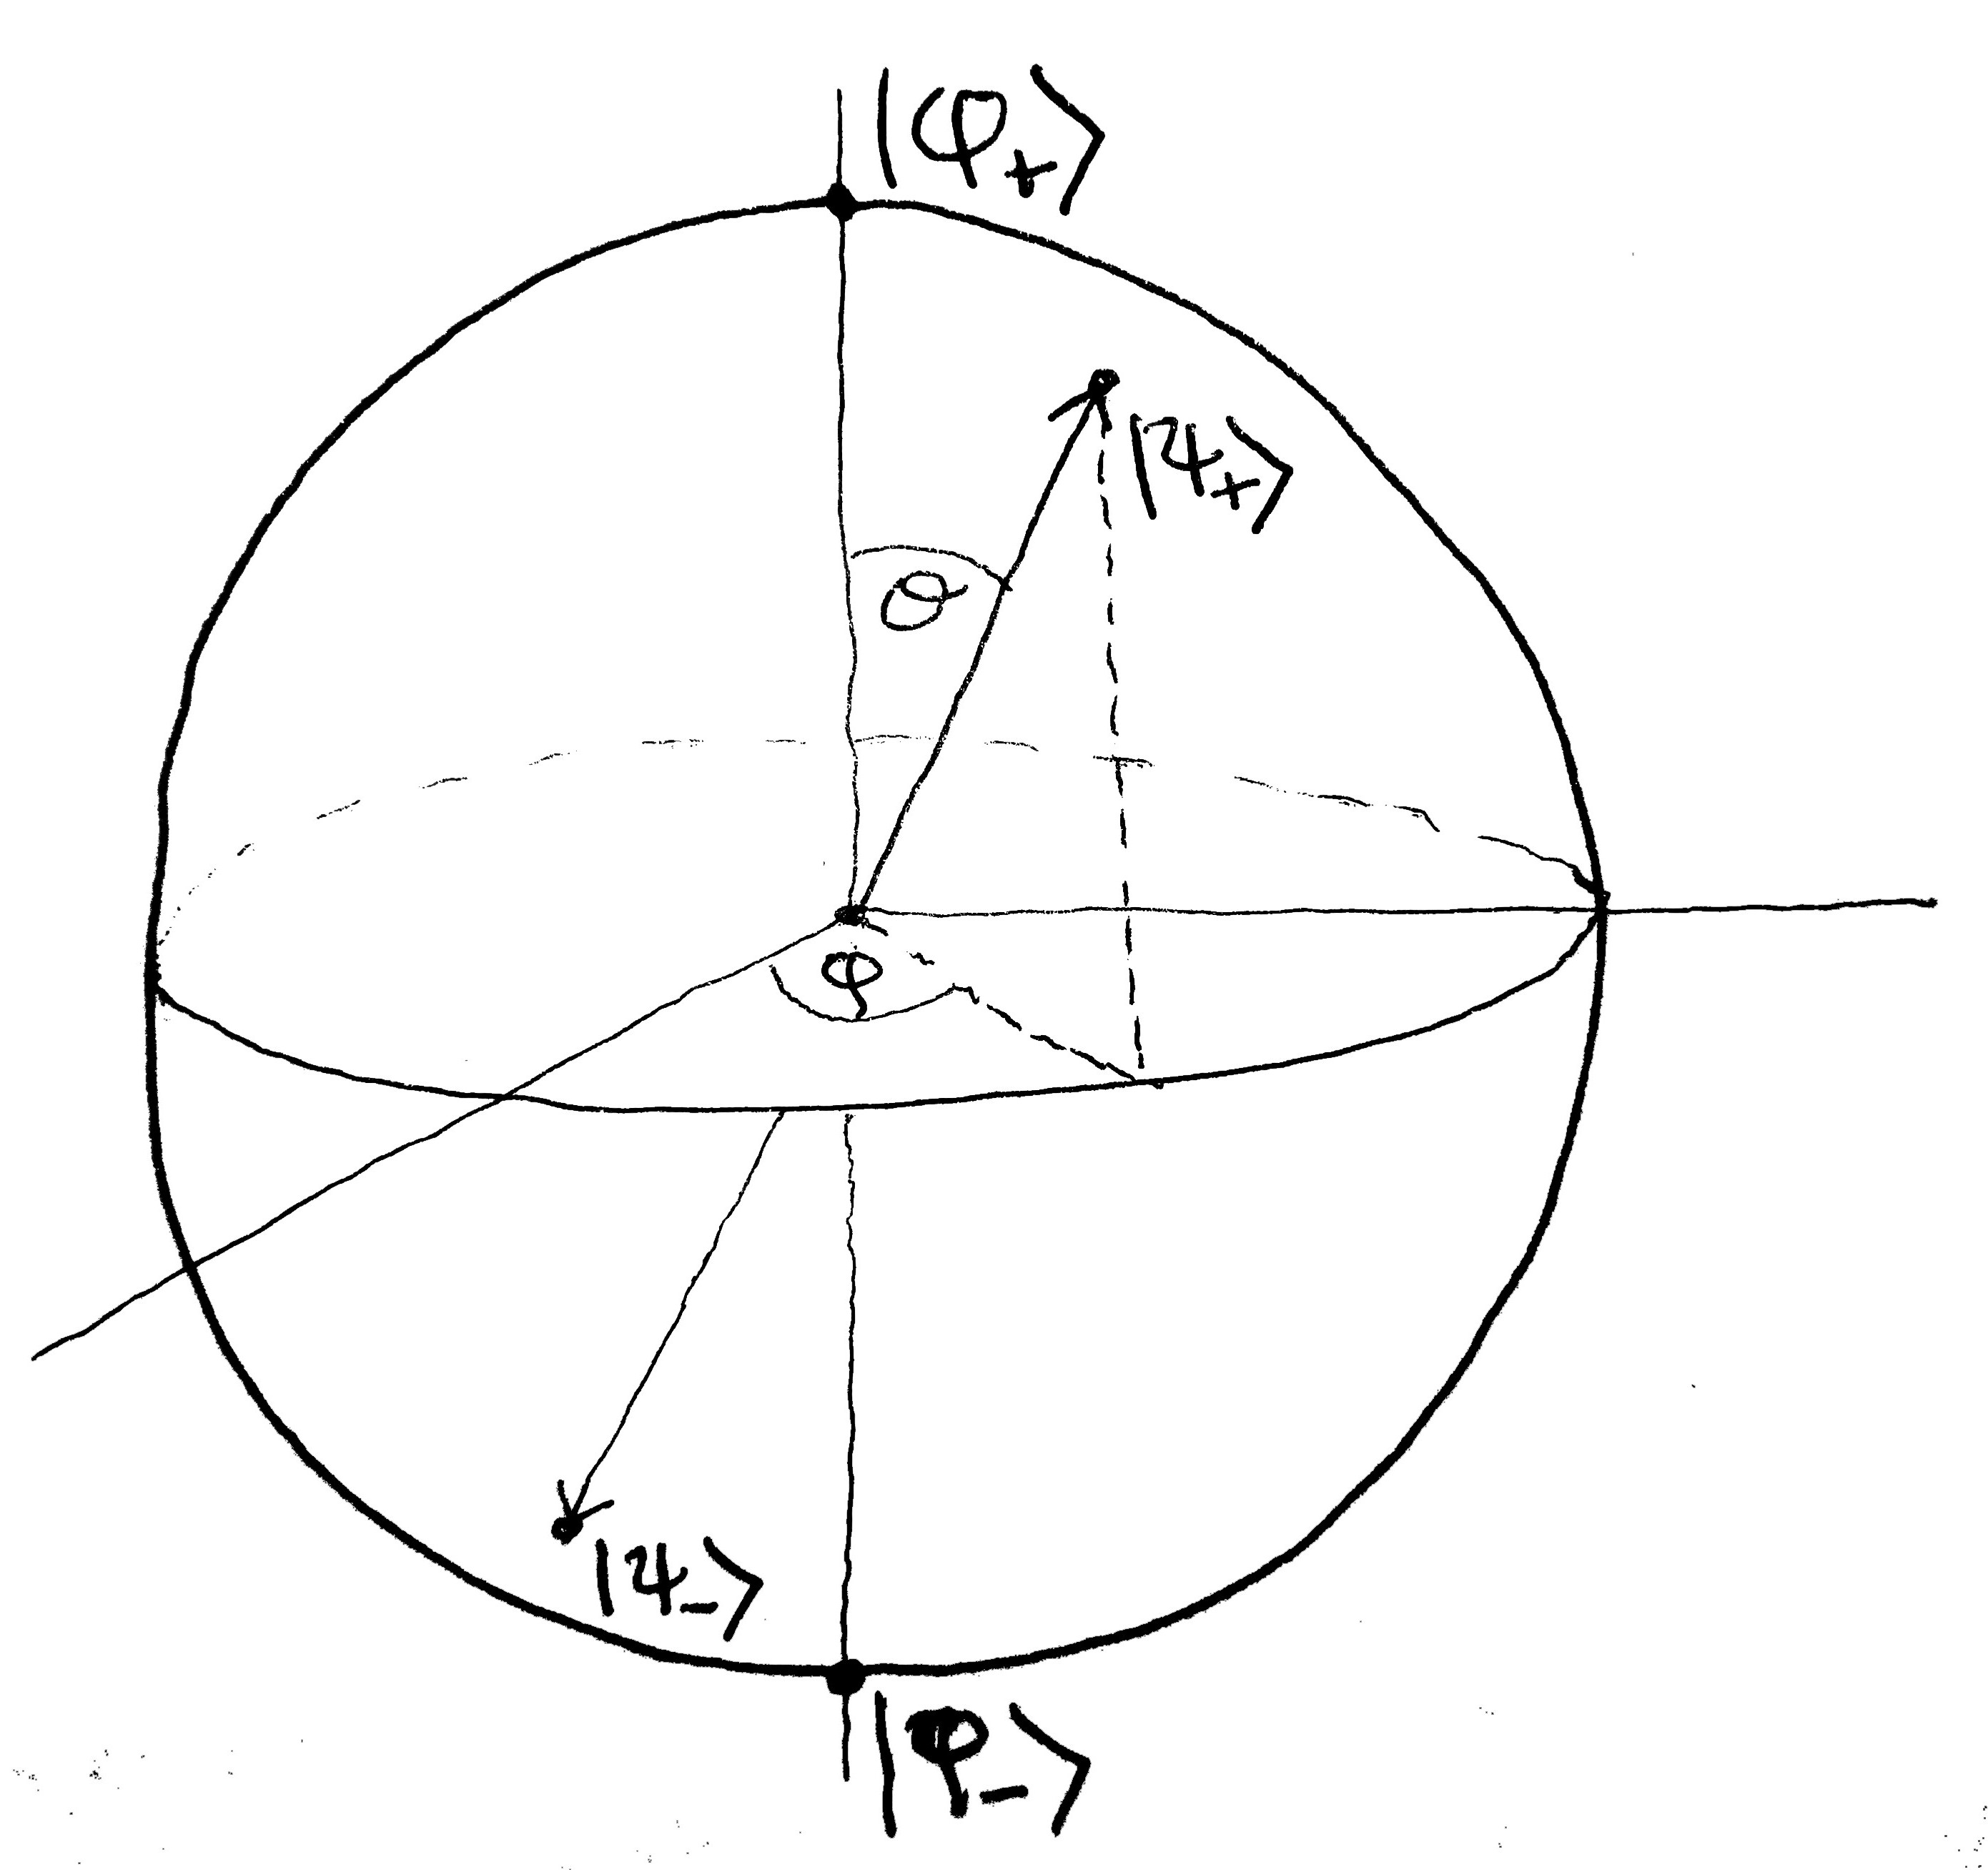
\includegraphics[width=0.5\linewidth]{arbitrary-2-level-system.jpg}
    \caption{Eigensystem of a general 2-level quantum system on the Bloch
        sphere. $\ket{\varphi_\pm}$ are the eigenstates of the pure-diagonal
        Hamiltonian (e.g. the spin Hamiltonian \eqref{eq:spin-hamiltonian}),
        while $\ket{\psi_\pm}$ are the eigenstates of the general Hamiltonian
        with off-diagonal elements.}%
    \label{fig:arbitrary-2-level-system}
\end{figure}
[Cohen-Tannoudji, Diu, Laloe; Quantum Mechanics Vol. 1]
Most general $2\times 2$ Hermitian matrix:
\[\hat{H} = \frac{1}{2} \pmqty{\xmat*{H}{2}{2}}
\qq{where} H_{12}^* = H_{21}, \qq{and} H_{11}, H_{22} \in \mathbb{R}\]
\[\qq{Take} H_{11} > H_{22} \qq{without loss of generality.}\]
Move zero of energy to midway between the levels:
\begin{alignat}{1}
    H \rightarrow \hat{H} -\frac{H_{11} + H_{22}}{4}\otimes\id
    &= \frac{1}{2}
    \pmqty{\frac{H_{11}-H_{22}}{2}&H_{12}\\H_{21}&\frac{-H_{11}+H_{22}}{2}}
    \\[2ex] &\equiv \frac{1}{2}
    \pmqty{\epsilon&\Delta-i\tilde{\Delta}\\ \Delta+i\tilde{\Delta}&-\epsilon}
    \\[2ex]
    &= \frac{\epsilon}{2} \hat{\sigma}_z
        + \frac{\tilde{\Delta}}{2}\hat{\sigma}_y
        + \frac{\Delta}{2}\hat{\sigma}_x
\end{alignat}
Take $H_0 = \frac{1}{2}\pmqty{\dmat[0]{\epsilon,-\epsilon}} =
\frac{\epsilon}{2}\hat{\sigma}_z$ with eigenvectors $\ket{\varphi_\pm}$,
\[H_0\ket{\varphi_\pm} = \pm \frac{\epsilon}{2} \ket{\varphi_\pm},\]
as the north and south pole of the Bloch sphere (see
Fig.~\ref{fig:arbitrary-2-level-system}. Then introduce the off-diagonals
\[H = H_0 + H_1, \qq{where} H_1
= \frac{1}{2}\pmqty{\admat[0]{\Delta-i\tilde{\Delta},\Delta+i\tilde{\Delta}}}.\]
Solve for the eigensystem:
\[H\ket{\psi_\pm} = E_\pm\ket{\psi_\pm}\]
\[\det\pmqty{\epsilon - 2E_\pm & \Delta - i\tilde{\Delta}
\\ \Delta + i\tilde{\Delta} & -\epsilon - 2E_\pm} = 0\]
\begin{alignat}{1}
    E_\pm &= \pm\frac{1}{2}\sqrt{\epsilon^2 + \Delta^2 + \tilde{\Delta}^2}
    \\[2ex]
    &\equiv \pm\frac{1}{2}\hbar\omega_q
\end{alignat}
\begin{alignat}{1}
    \ket{\psi_+} &= e^{-i\varphi/2}\cos\frac{\theta}{2}\ket{\varphi_+}
        + e^{i\varphi/2}\sin\frac{\theta}{2}\ket{\varphi_-}
    \\[2ex]
    \ket{\psi_-} &= e^{-i\varphi/2}\sin\frac{\theta}{2}\ket{\varphi_+}
        + e^{i\varphi/2}\cos\frac{\theta}{2}\ket{\varphi_-}
\end{alignat}
This orients the $\ket{\psi_\pm}$ axis at polar angle $\theta$ and azimuthal
angle $\varphi$ relative to the $\ket{\varphi}$ axis (see
Fig.~\ref{fig:arbitrary-2-level-system}), where
\begin{alignat}{1}
    \tan\theta &= \frac{\sqrt{\Delta^2 + \tilde{\Delta}^2}}{\epsilon} \\
    \tan\varphi &= \frac{\tilde{\Delta}}{\Delta}
\end{alignat}

\subsection{Spin in a generalized magnetic field}
We can map the results of Sec.~\ref{sec:arbitrary-2-level-system} to the spin
problem as follows:
\begin{alignat}{1}
    \ket{\uparrow} &\longrightarrow \ket{\varphi_+} \\
    \ket{\downarrow} &\longrightarrow \ket{\varphi_-} \\
    \ket{\uparrow}_y &\longrightarrow \ket{\psi_+} \\
    \ket{\downarrow}_y &\longrightarrow \ket{\psi_-} \\
    \hbar\gamma B &\longrightarrow \hbar\omega_q \\
    B_z &\longrightarrow \epsilon \\
    B_x &\longrightarrow \Delta \\
    B_y &\longrightarrow \tilde{\Delta} \\
\end{alignat}
\[H = -\frac{\gamma\hbar}{2}\pmqty{B_z & B_x - iB_y \\ B_x + iB_y& - B_z}\]
With a static field $\vec{B} = B_x\hat{x} + B_y\hat{y} + B_z\hat{z}$, a general
state just precesses about the new eigenaxis (the $\ket{\psi_\pm}$ axis in
Fig.~\ref{fig:arbitrary-2-level-system}). With a time-dependent perturbation in
the field, $\vec{B} = B_z\hat{z} + B_1\cos(\omega_0t)\hat{x}$ where $B_1 \ll
B_0$, we can get fast precession about the $z$-axis and slow precession about
the $x$-axis.


\subsection{LC oscillator as a superconducting qubit}
Frequency: $f = 1/\sqrt{LC} \sim \hbar\omega$.
\[\hat{H} = \frac{1}{2} \hbar\omega_a\hat{\sigma}_z +
\hbar\Omega_R\cos(\omega_0t+\Phi_R)\hat{\sigma}_x\]

LC oscillator has same spectrum as simple harmonic oscillator; evenly-spaced
energy levels. Need to introduce anharmonicity via a nonlinear component to
break this even spacing so that a single transition between 2 specific levels
(qubit) can be addressed. This nonlinear component is the Josephson junction,
characterized by a current-phase relationship (CPR).

\subsection{Quantum LC circuit}
** This section is needed to make chapter 4 a little easier to understand. The introductory section of wikipedia's article on this is actually pretty sufficient at supplying basic definitions here.


\subsection{Example}

Question:
\\\\
Suppose that you have a system of N qubits. How many classical bits does it take to describe the state of the system? First, consider a quantum register containing three qubits, each of which is prepared in state
\begin{equation}
    \frac{\ket{0} +\ket{1}  }   {\sqrt{2}}
\end{equation}

You perform a measurement that projects each qubit onto either $\ket{0}$ or  $\ket{1}$ and
record the result in a 3-bit classical register. List all possible outcomes.
\\
\\

Answer:\\

First we consider a system of 3 qubits, all of them in the state $(|0\rangle +|1\rangle)/\sqrt{2}$, so the combined wave function is:
\begin{equation}
    |\psi \rangle = \frac{1}{2\sqrt{2}}\left(|000\rangle+|001\rangle+|010\rangle+|011\rangle+|100\rangle+|101\rangle+|110\rangle+|111\rangle \right).
\end{equation}
If we measure each qubit in the $\{|0\rangle,|1\rangle\}$ basis, we can have 8 possible outcomes: $|000\rangle$, $|001\rangle$, $|010\rangle$, $|011\rangle$, $|100\rangle$, $|101\rangle$, $|110\rangle$, $|111\rangle$ all with probability $1/8$.

In general, the Hilbert space of $N$ qubits can be expanded as the tensor product of the Hilbert spaces of each of its qubits. This allows us to define a basis in the space of all qubits as the tensor product of all the possible combinations of the basis elements of the single qubit states: $\{|000\rangle,|001\rangle,|010\rangle,|011\rangle,|100\rangle,|101\rangle,|110\rangle,|111\rangle\}$ in the case of three qubits. In a system of $N$ qubits the number of basis elements is therefore $\boldsymbol{2^N}$. Therefore, to fully characterize the state of an $N$ qubit system we need to specify $2^N$ complex numbers (or, more precisely, $2^{N} - 1$ due to the normalization constraint and the ability to ignore an overall global phase, which removes two real parameters, or equivalently one complex parameter). Because the parameters specifying the state are continuous, they cannot be represented precisely/exactly with a finite number of bits, in general.

This exponential scaling of the size of the Hilbert space with the number of qubits is the reason why it is not possible to efficiently simulate quantum computers with classical ones.

A final note about representing a many-body quantum state with a finite number of bits: we are making a rounding error on each component of the wave function, therefore the wave function  that we are representing is an approximation ($|\psi_{\textrm{Approx}} \rangle$) to the exact one ($|\psi \rangle$). We want to have a good approximation so: $\langle \psi_{\textrm{Approx}}|\psi \rangle \sim 1$. However, this approximation gets intrinsically worse as the number of qubits increases if the precision in the bits is not increased. This a consequence of something known as the \textbf{orthogonality catastrophe}. Imagine we can represent our single qubit states with an error $\varepsilon$:
$$\langle \psi_{\textrm{Approx}}^{(i)}|\psi ^{(i)} \rangle = 1-\varepsilon,$$ 
where $(i)$ labels qubit $(i)$. If we form a many-qubit state as the product of the approximate states, its overlap will decay exponentially with the number of qubits:
\[\langle \psi_{\textrm{Approx}}|\psi  \rangle = (1-\varepsilon)^N \sim e^{-\varepsilon N}.\]
Therefore to accurately describe our quantum many-body states we need a lot of classical bits for each of the exponentially many wave function components.






%ANDREAS TSANTILAS
%7/20/20


%hi
%hello
\subsection{The Quantum Zeno Effect}
It has been previously discussed that measuring a qubit in the $\{\ket{0}, \ket{1}\}$ basis corresponds to projecting its state $\ket{\psi}$ onto one of the basis vectors. This projection implies a way to ``preserve" the state of a quantum system \cite{zeno}. Let's consider the simplest type of decay possible: suppose we have a qubit in the state $\ket{0}$ that constantly tries to decay to the state $\ket{1}$. In time $\Delta t$, our qubit will rotate very slightly, let's say by angle $\theta = \epsilon$.

If we let enough time elapse, as $\theta \to \pi/2$, the greater the chance of measuring $\ket{1}$ becomes, which would correspond to qubit decay. However, if we periodically measure the state after short time intervals $\Delta t$, the state will only have time to rotate by $\epsilon$. Then, the probability that the state $\ket{\psi} = \cos(\epsilon)\ket{0} + \sin(\epsilon)\ket{1}$ is measured to be $\ket{0}$ is $\cos^2(\epsilon) \approx 1-\epsilon^2$, which, as $\epsilon$ becomes arbitrarily small, becomes closer and closer to certainty.

In the limiting case, as the period between measurements $\Delta t\to 0$, we arrive at an interesting result: if a quantum system is observed continuously, then it will \textit{never} decay!

Experimentally, this has been verified multiple times. In the next section, we will see a result that encapsulates 

\subsection{The Elitzur-Vaidman Bomb}

How can you eat your cake and have it too? 

That is (essentially) the question Avshalom Elitzur and Lev 
Vaidman, two Israeli physicists, set out to solve. They proposed a thought experiment in 
which one could verify a bomb is functional without having to detonate it \cite{Elitzur_1993}. A crucial concept that 
this experiment demonstrates is that of \textit{interaction-free measurement}.

Traditionally, the setup involves mirrors, detectors, and a light-sensitive bomb, which detonates if it interacts with even 
a single proton. Angled half-silvered mirrors are used to place each photon in an equal superposition 
state of travelling upwards, and travelling through the bomb. From that, we can use the interference of these waves in a 
clever way to determine if a bomb is a dud or not, with exploding good bombs only half the time! 

However, there is another setup more amenable to quantum circuits such that the proportion of bombs 
exploded can be made \textit{arbitrarily small}. It is this setup that will be considered \cite{scaaronson}.


\subsubsection{The Classical Setup}

Suppose you are at an airport, and there is a suspicious piece of luggage left lying around. This 
suitcase may or may not contain a bomb; of course, if you open the suitcase, the bomb explodes. 

The suitcase does, however, have an interface. It can be sent a classical bit, 
\[
b \in \{0,1\}    
\]
where $b=0$ means we don't make a query, and $b=1$ means we do. This is a predicament; if we send 0, we don't 
learn anything, and if we send 1, we risk the bomb blowing up in our face! 

For the sake of abstraction, the suitcase can be represented by a ``black box," 
whose contents are unknown. There are two classical bits in the circuit: our input $b$ and 
one that gets measured. The way we denote an ``explosion" is if we measure the second bit 
in the state 1. Note that the act of measuring 1 sets off the bomb, not that the output bit is 1. The corresponding circuits look like:

\begin{center}
    \begin{quantikz}[thin lines]
        \lstick{$b$} &\qw & \qw\gategroup[wires=2,steps
        =3,style={inner sep=6pt}]{No Bomb}  & \qw & \qw & \qw &\qw &\qw  \\
        
        &&&\lstick{0}& \qw & \qw & \qw & \meter{}
    \end{quantikz}
\end{center}

\begin{center}
    \begin{quantikz}[thin lines]
        \lstick{$b$} &\qw & \qw\gategroup[wires=2,steps
        =3,style={inner sep=6pt}]{Bomb}  & \qw & \ctrl{1} & \qw &\qw &\qw  \\
        &&&\lstick{0}& \targ{} &\qw & \qw & \meter{}
    \end{quantikz}
\end{center}

Think about what happens. If there is no bomb, and we send in $b=0$, then we measure zero. 
If there is a bomb, and we send in $b=0$, then we \textit{also} measure 0. So sending in $b=0$ doesn't give 
us any information about what's going on inside. If there is no bomb, and we send in $b=1$, then we measure 
zero. We can say for certain, then, that there isn't a bomb. If there is a bomb, and $b=1$, then the suitcase 
explodes. This is very unhelpful, and is equivalent to just opening up the suitcase to see for yourself.


\subsubsection{The Quantum Setup}

Let's suppose the query system is a quantum one. That is, we are allowed to send in 
a quantum bit 

\[\ket{\psi} = \alpha \ket{0} + \beta \ket{1}\] 

to our suitcase. Let's assume that if there is no bomb, then
$\ket{\psi}$ is returned. If there is a bomb, the bomb measures the second qubit in the basis 
$\{\ket{0}, \ket{1}\}$. If the outcome is $\ket{0}$, then because the states of 
the two qubits are entangled, our qubit $\ket{\psi}$ immediately collapses to $\ket{0}$ and therefore returns 
$\ket{0}$. If the output is $\ket{1}$, the bomb explodes (and then returns \ket{1}).

Our corresponding quantum circuits look like:

\begin{center}
    \begin{quantikz}[thin lines]
        \lstick{$\ket{\psi}$} &\gate{R(\epsilon)} & \qw\gategroup[wires=2,steps
        =3,style={inner sep=6pt}]{No Bomb}  & \qw & \qw & \qw &\qw &\gate{Return} \\
        &&&\lstick{$\ket{0}$}& \qw & \qw & \qw & \meter{}
    \end{quantikz}
\end{center}

\begin{center}
    \begin{quantikz}[thin lines]
        \lstick{$\ket{\psi}$} &\gate{R(\epsilon)} & \qw\gategroup[wires=2,steps
        =3,style={inner sep=6pt}]{Bomb}  & \qw & \ctrl{1} & \qw &\qw &\gate{Return}  \\
        &&&\lstick{$\ket{0}$}& \targ{} &\qw &\qw & \meter{} 
    \end{quantikz}
\end{center}

How do we go about testing if there is a bomb? The idea is to start in the state $\ket{\psi} = \ket{0}$.
Next, we apply an arbitrarily small rotation of angle $\epsilon = \frac{\pi}{2N}$, where $N$ 
is the nubmer of times we will repeat this process, and is arbitrarily large. The matrix is

\[
R(\epsilon)  =  \begin{pmatrix}
    \cos(\epsilon) & -\sin(\epsilon)\\
    \sin(\epsilon)  & \cos(\epsilon)
\end{pmatrix}
\]

giving us $\ket{\psi} = \cos(\epsilon)\ket{0} + \sin(\epsilon)\ket{1}$. If there is a 
bomb, the chance that it explodes is $\sin^2(\epsilon) \approx \epsilon^2$. With a high probabiltiy, we 
get back $\ket{0}$ and put that back into the black box.\footnote{That is, unless you live in the
unlucky branch of the multiverse where it explodes! The authors of \cite{Elitzur_1993} argue that the part of the superposition where the bomb explodes actually occurs, just not in our ``world." Generally, this is known as the \textit{Many-Worlds Interpretation} (MWI) of quantum mechanics. It has never been tested and is hotly debated among scientists.}

Now let's repeat this process $N$ times, and then we measure our $\ket{\psi}$ safely 
in our lab. 

If there is no bomb, then our state is 
\[
R^N(\epsilon)\ket{0} = R(N\epsilon)\ket{0} = R(\pi/2)\ket{0} = \ket{1}    
\]
and we measure $\ket{1}$ in our lab. 

If there is a bomb, however, each time we measure we ``reset'' the state of our qubit
back to $\ket{0}$. Therefore, the total probability of setting off our bomb is only 

\[
N\sin^2(\epsilon) \approx N\epsilon^2 = \frac{\pi^2}{4N}  = O\left(\frac{1}{N}\right)  .
\]

In conclusion, if there is no bomb, we measure $\ket{1}$ in our lab after doing $N$ repetitions, and if there is, 
we measure $\ket{0}$ in our lab since the circuit keeps resetting the state of $\ket{\psi}$ to zero. If we do 
100 repetitions, then our chance of exploding (if there is a bomb) is about $2.47\%$. I like 
those odds!

\subsubsection{Qiskit Implementation}
Below is the implementation of this in Qiskit. 

\begin{lstlisting}[numbers=none]
N = 10
epsilon_ = np.pi/(2*N)
isBomb = False


def run_ev_circ(isBomb):
    qr = QuantumRegister(1, 'q')
    cr = ClassicalRegister(1,'c')
    qc = QuantumCircuit(qr,cr)
    if (isBomb):
        qc.ry(2*epsilon_,0)
        qc.measure(0,0)
    else:
        qc.ry(2*N*epsilon_,0)
        qc.measure(0,0)

    simulator = Aer.get_backend('qasm_simulator')
    job = execute(qc, simulator, shots=N*1000)
    result = job.result()
    counts = result.get_counts(qc)
    return counts
\end{lstlisting}









\section{Multiple qubits}
\footnote{10/16/19}Enormous difference in dimension between classical and
quantum state space is due to a difference in the way the spaces combine.

The state of a classical system can be completely characterized by describing
the state of each of its component pieces separately.

An unintuitive aspect of quantum systems is that often the state of the system
cannot be described in terms of the state of its component pieces $\implies$
\emph{entangled states}.

Feynman/Manin said classical systems cannot simulate entangled states in
polynomial time (due to the scaling of the Hilbert space dimension with system
size). $n$ qubits $\implies 2^n$ states, $2^n \times 2^n$ dimensional Hilbert
space.

Classical system of $n$ objects whose individual state can be described in 2D
vector space $\implies$ $2n$. \emph{Direct sum}, $\oplus$.

Quantum system of $n$ objects $\implies$ $2^n$. \emph{Tensor product},
$\otimes$.

\subsection{Direct sum of vector spaces}
\renewcommand*{\VV}{\mathbb{V}}
\newcommand*{\WW}{\mathbb{W}}

\[\VV: A = \{\ket{\alpha_1}, \ket{\alpha_2}, \ldots, \ket{\alpha_n}\}\]
\[\WW: B = \{\ket{\beta_1}, \ket{\beta_2}, \ldots, \ket{\beta_n}\}\]
Every element $\ket{x} \in \VV \oplus \WW$ can be written as $\ket{x} = \ket{v}
\oplus \ket{w}$ for some $\ket{v} \in \VV$ and $\ket{w} \in \WW$.

Suppose the state of three objects $O_1, O_1, O_3$ is fully described by two
parameters, the positions $x_i$ and the momenta $p_i$. Then the state of the
system can be described by direct sum of the states of the individual objects,
\[\pmqty{x_1\\p_1} \oplus \pmqty{x_2\\p_2} \oplus \pmqty{x_3\\p_3}
= \pmqty{x_1\\p_1\\x_2\\p_2\\x_3\\p_3}\]
$\implies$ state of $n$ classical objects (each with 1 degree of freedom) has
dimension $2n$.

\subsection{Tensor products of vector spaces}
The tensor product $\VV \otimes \WW$ of two vecor spaces $\VV$ and $\WW$ with
bases $A = \{\ket{\alpha_1}, \ldots, \ket{\alpha_n}\}$ and  $B =
\{\ket{\beta_1}, \ldots, \ket{\beta_m}\}$ respectively is an $nm$-dimensional
vector space with a basis consisting of $nm$ elements of the form
$\ket{\alpha_i} \otimes \ket{\beta_j}$ where $\otimes$ is the tensor product.
All elements of $\VV \otimes \WW$ can be represented:
\[a_{11} \ket{\alpha_1} \otimes \ket{\beta_1} + a_{12} \ket{\alpha_1} \otimes
\ket{\beta_2} + \cdots + a_{nm}\ket{\alpha_n} \otimes \ket{\beta_m}\]

The standard basis for the vector space $\VV_{n-1} \otimes \VV_{n-2} \otimes
\cdots \otimes \VV_0$ for an $n$-qubit (i.e. 2-level, size 2 basis) system
consists of $2^n$ vectors:
\[\ket{0}_{n-1} \otimes \cdots \otimes \ket{0}_1 \otimes \ket{0}_0\]
\[\ket{0}_{n-1} \otimes \cdots \otimes \ket{0}_1 \otimes \ket{1}_0\]
\[\ket{0}_{n-1} \otimes \cdots \otimes \ket{1}_1 \otimes \ket{0}_0\]
\[\vdots\]
\[\ket{1}_{n-1} \otimes \cdots \otimes \ket{1}_1 \otimes \ket{1}_0\]
Every $n$-qubit quantum state can be represented:
\[e^{i\theta}(a_0\ket{000\ldots0} + \cdots + a_{2^n-1} \ket{111\ldots1})\]
$\implies$ $2^n - 1$ complex numbers (global phase + normalization condition
removes 2 real numbers).

If Alice controls 2 qubits and Bob the last three we may write a state as
\[ \frac{1}{\sqrt{2}} \left( \ket{00}_A\ket{101}_B +
\ket{10}_A\ket{011}_B\right)\]
where the subscripts indicate which qubits Alice controls and which Bob
controls.

\subsection{Meaning of entanglement}
\textbf{Bell basis} for a two-qubit system:
\begin{equation}\begin{gathered}
\ket{\Phi^+} = \frac{1}{\sqrt{2}} (\ket{00} + \ket{11}) \\
\ket{\Phi^-} = \frac{1}{\sqrt{2}} (\ket{00} - \ket{11}) \\
\ket{\Psi^+} = \frac{1}{\sqrt{2}} (\ket{01} + \ket{10}) \\
\ket{\Psi^-} = \frac{1}{\sqrt{2}} (\ket{01} - \ket{10})
\label{eq:bell-basis}
\end{gathered}\end{equation}

The elements of the Bell basis are entangled. For instance $\ket{\Phi^+}$
cannot be described in terms of the state of its component qubits separately
(i.e. in terms of a product state).

\footnote{10/21/19}Example 4-qubit state:
\begin{alignat}{1}
    \ket{\psi} &= \frac{1}{2}
        (\ket{0000} + \ket{0101} + \ket{1010} + \ket{1111}) \\
    &= \frac{1}{\sqrt{2}} (\ket{0}_1\ket{0}_3 + \ket{1}_1\ket{1}_3) \otimes
        \frac{1}{\sqrt{2}} (\ket{0}_2\ket{0}_4 + \ket{1}_2\ket{1}_4)
\end{alignat}
$\implies$ $\ket{\psi}$ is not entangled with respect to the system composition
of a subsystem of the 1st \& 3rd qubit and a subsystem of the the 2nd \& 4th
qubit.

\subsubsection{Multi-qubit measurements}
Two qubits:
\[\ket{\psi} = a\ket{00} + b\ket{01} + c\ket{10} + d\ket{11}\]
\[\abs{a}^2 + \abs{b}^2 + \abs{c}^2 + \abs{d}^2 = 1\]
We wish to measure the 1st qubit with respect to the standard basis $\{\ket{0},
\ket{1}\}$. Let $\VV_1, \VV_2$ be the vector spaces of the 1st and 2nd qubits,
respectively. Then $\VV = \VV_1 \otimes \VV_2$ is the vecotr space of the
composite system.
\[S_1 = \ket{0} \otimes \VV_2, \qquad S_2 = \ket{1} \otimes \VV_2\]
\[\ket{\psi_1} = \frac{a}{c_1}\ket{00} + \frac{b}{c_1}\ket{01} \in S_1\]
\[\ket{\psi_2} = \frac{c}{c_2}\ket{10} + \frac{d}{c_2}\ket{11} \in S_2\]
\[\ket{\psi} = c_1\ket{\psi_1} + c_2\ket{\psi_2}\]
\[c_1 + \sqrt{\abs{a}^2 + \abs{b}^2}, \qquad
c_2 + \sqrt{\abs{c}^2 + \abs{d}^2}\]
\[\implies \ket{\psi} = \ket{0} \otimes (a\ket{0} + b\ket{1})
+ \ket{1} \otimes (c\ket{0} + d\ket{1})\]
Multi-bit measurement can be treated as a series of single-bit measurements in
standard basis.
\begin{itemize}
    \item Measure if two qubits have the same value without learning the actual
        value of the two qubits.
    \item Equivalent to unitary transformations followed by a standard
        measurement of individual qubits.
\end{itemize}

Measurement gives another way of thinking about entangled particles. Particles
are not entangled if the measurement of one has no effect on the other. For
example, the state $(\ket{00} + \ket{11}) / \sqrt{2}$ is entangled since the
probability that the first bit is measured to be $\ket{0}$ is 1/2 if the second
bit has not been measured. However, if the second bit had been measured, the
probability would be 0 or 1. On the other hand, the state $(\ket{00} +
\ket{01}) / \sqrt{2} = \ket{0} \otimes (\ket{0} + \ket{1}) / \sqrt{2}$ is not
entangled, since any measurement of the first qubit will yield $\ket{0}$
regardless of whether the second qubit was measured.

\subsubsection{EPR paradox}
Einstein, Podolsky, and Rosen proposed a thought experiment that uses entangled
particles which seem to violate principles of relativity.
\[ A \longleftarrow \text{EPR source} \longrightarrow B\]
The EPR source generates two maximally entangled particles,
\[\frac{1}{\sqrt{2}} (\ket{00} + \ket{11}).\]
$A$ and $B$ can be arbitrarily far apart.

Suppose $A$ measures her particle and observes state $\ket{0}$. $\implies$
means the combined state will now be $\ket{00}$. Now if B measures his
particle, he will observe $\ket{0}$.

The change of the combined quantum state occurs instantaneously even though the
particles may be arbitrarily far apart. It appears that this would enable $A$
and $B$ to communicate faster than the speed of light. (Actually, they can't.)

EPR proposed local hidden variable theory. Each particle has some internal
state that completely determines what the result of the measurement will be,
but these variables are hidden from us. For the moment, the best we can do is
to make probabilistic predictions.

J.~S. Bell showed that the EPR picture must satisfy an inequality (now known as
Bell's inequality). This inequality has been experimentally violated $\implies$
EPR cannot explain the results of measurements with respect to a different
basis.

Description of \emph{cause and effect}. A measurement by Alice affects a
measurement performed by Bob. It is possible to set up the EPR scenario so that
one observer \emph{sees} Alice measure first, while another observer
\emph{sees} Bob measure first. According to relativity, physics must explain
equally well the observation of the first observer as the second. The
experimental results should be explained equally. The symmetry shows that Alice
and Bob cannot use their EPR pair to communicate faster than the speed of
light. All that can be said is that Alice and Bob are observing the same random
(though perfectly correlated) behavior.


\section{Quantum gates}
Quantum systems obey Schr\"odinger's equation. The dynamics must take states to
other states in a way that preserves orthogonality (unitary dynamics). For a
complex vector space, linear transformation, unitary.

Suppose matrix $M$ is unitary. $\implies$ $MM^\dag = \id$. $\implies$ quantum
transformations (e.g. gates) are unitary and therefore reversible. $\implies$
\emph{Energy of computation}. Classical computation is \emph{not} reversible.

\subsection{Single-qubit gates}
Computational basis $\{\ket{0}, \ket{1}\}$.

\begin{center}
\begin{tabular}{llll}
    $\id$
    & $\mqty{\ket{0}\rightarrow\ket{0} \\ \ket{1}\rightarrow\ket{1}}$
    & $\pmqty{\imat{2}}$
    & identity
    \\[5ex] $X$
    & $\mqty{\ket{0}\rightarrow\ket{1} \\ \ket{1}\rightarrow\ket{0}}$
    & $\pmqty{\pmat{1}}$
    & negation
    \\[5ex] $Y$
    & $\mqty{\ket{0}\rightarrow&-\ket{1} \\ \ket{1}\rightarrow&\ket{0}}$
    & $\pmqty{0&1\\-1&0}$
    & note: not Pauli
    \\[5ex] $Z$
    & $\mqty{\ket{0}\rightarrow&\ket{0} \\ \ket{1}\rightarrow&-\ket{1}}$
    & $\pmqty{\pmat{3}}$
    & phase flip
\end{tabular}
\end{center}

\footnote{10/23/19}Hadamard gate:
\begin{center}\begin{tabular}{llll}
    $H$
    & $\mqty{\ket{0}\rightarrow&\ket{+} \\ \ket{1}\rightarrow&\ket{-}}$
    & $\displaystyle\frac{1}{\sqrt{2}} \pmqty{1&1\\1&-1}$
    & Hadamrd gate
\end{tabular}\end{center}

Quantum transformations are unitary transformations:
\begin{itemize}
    \item Invertible/reversible: $U^\dag U = \id \implies U^\dag = U^{-1}$.
    \item Deterministic.
    \item Continuous: you can apply them in a time-continuous way.
\end{itemize}
Measurements break all three rules of unitary transformations:
\begin{itemize}
    \item Irreversible: whatever information we didn't capture is lost.
    \item Probabilistic: QM is deterministic only until measurement.
    \item Discontinuous: measurement is assumed to project instantaneously.
\end{itemize}

Norms:
\begin{itemize}
    \item $p$-norm: $\abs{x}_p = (\sum_i \abs{x_i}^p)^{1/p}$
    \item 1-norm: $\abs{x} = \sum_i \abs{x_i}$ (classical probability)
    \item 2-norm: $\abs{x}_2 = \sqrt{\sum_i \abs{x_i}^2}$ (QM)
\end{itemize}

Quantum circuit notion: (quantum circuit diagram).

\subsection{Two-qubit gates}
** Would be worth mentioning noise from CNOT gate (and others?)
** Subsection on phase kickback
** Should have subsections covering S-gate, T-gate, U-gates
Controlled NOT (CNOT) gate. First qubit is control bit:
\begin{alignat}{1}
    \ket{00} &\rightarrow \ket{00} \\
    \ket{01} &\rightarrow \ket{01} \\
    \ket{10} &\rightarrow \ket{11} \\
    \ket{11} &\rightarrow \ket{10}
\end{alignat}
\[C_\text{NOT} = \pmqty{\mqty{\imat{2}}&\mqty{\zmat{2}{2}}
                    \\ \mqty{\zmat{2}{2}}&\mqty{\pmat{1}}}
            = \pmqty{\id&0\\0&X}\]
\[C_\text{NOT}C_\text{NOT} = \id\]
The CNOT gate cannot be decomposed into a tensor product of two single qubit
transformations.

(Matrix representations of 2-qubit gates constructed as tensor products of
single-qubit gates. Connection between operator/Dirac notation and matrix/array
representations.)

** A fun(?) exercise or optional subsection here should be made on proving universality. IBM's qiskit textbook does this in a pretty easy-to-follow way that isn't so rigorous if the authors don't care too much about mathematical rigor. 


\section{Quantum Communication}
%$\ldots$


\vspace{2ex}\noindent
\fbox{\footnote{9/16/19}App.~\ref{sec:python}.}

%\footnote{9/18/19}(Notes missing.)

\subsection{Example}


Question :


\newcommand*{\HH}{\leftrightarrow}
\newcommand*{\VV}{\updownarrow}
\newcommand{\Dzero}{%
  \mathrel{\text{\ooalign{$\swarrow$\cr$\nearrow$}}}%
}
\newcommand{\Done}{%
  \mathrel{\text{\ooalign{$\searrow$\cr$\nwarrow$}}}%
}
\renewcommand{\arraystretch}{1.4}
\newcommand*{\X}{$\times$}
\newcommand*{\G}[1]{\textcolor{Green4}{#1}}
\newcommand*{\R}[1]{\textcolor{Red4}{#1}}

Alice and Bob have two methods of communication: they can communicate classically (by text messages) and they can communicate quantumly (Alice can send Bob single photons over an optical fiber). It is possible for other people to hack into both of these methods of communication. They agree that Alice will encode a string of `0's and `1's in the polarization state of photons. If they can verify no one intercepted this string, they will use it as their secret key. They agree to use the following mapping:
\begin{equation}
    \ket{{\HH}} \rightarrow 1 
\end{equation}
\begin{equation}
    \ket{\VV} \rightarrow 0
\end{equation}
    
Alice will send a photon with its polarization oriented either horizontally or vertically. She will choose the polarization randomly, with equal probability for either. She will also text Bob telling him that she sent a photon, without telling which polarization she sent. Bob will measure the photon and text her back to confirm that he received it, without telling her anything about how he measured the photon or the measurement outcome.
\begin{enumerate}[label=\textbf{\alph*.}]
    \item How can Bob measure the polarization of the photon that Alice sends? List two ways and explain why one would be better than the other.
    \item If Bob measures a vertically polarized photon, with what percent certainty does he know which polarization Alice sent?
    \item Now suppose there's an eavesdropper named Eve. She is able to intercept the
photon Alice sends to Bob, detect it, and send Bob a replacement photon. If she
overhears all of the discussions Bob and Alice have about their plan to share the secret key, is it possible for her to know the polarization state of every photon Alice sends with 100$\%$ certainty?
    \item  Assuming that Eve is able to send the replacement photon instantaneously, would Alice and Bob know that she has eavesdropped? Why or why not?
    \item Explain why it is not secure for Alice to tell Bob in which basis she is sending
photons.
    \item In the BB84 protocol, Alice and Bob still have the same two ways of
communicating (text messages and single photons), but Alice now has an additional
choice of sending light polarized horizontally, vertically, or with one of the two diagonal
polarizations. They agree to use the same mapping as in Equation 1 for horizontally
or vertically polarized photons, and the following mapping for the diagonally polarized
photons:

\begin{equation}
    \ket{\Dzero} \rightarrow 0
\end{equation}
\begin{equation}
    \ket{\Done} \rightarrow 1
\end{equation}


Alice now randomly sends any of the four polarization states with equal probability.
Bob doesn't know which basis Alice used, so he randomly chooses a basis (horizontal/vertical or diagonal) in which to measure the photon.

    \item Fill in the empty spaces in the following table. What is the secret key that Alice and Bob generate?
    
    
    \begin{table}
    \begin{threeparttable}
    \centering
    \begin{tabular}{c||c|c|c|c|c|c|c|c|c}
        Alice's bit &
        1 & 1 & 0 & 1 & 0 & 0 & 0 & 1 & 0 \\
        \hline\hline
        Alice's basis &
        $+$ & \X & \X & $+$ & \X & $+$ & $+$ & \X & \X \\
        \hline
        Alice's polarization &
        $\HH$ & $\Done$ & $\Dzero$ & &  &  &  &  &  \\
        \hline
        Bob's basis &
        \X & \X & $+$ & $+$ & $+$ & \X & $+$ & \X & $+$ \\
        \hline
        Bob's measurement &
        $\Done$ & $\Done$ & $\VV$ &  &
        {$\Dzero$} & $\Done$ &  &  & $\HH$ \\
        \hline
        Same basis? &
        No & Yes &  &  &  &  &  &  & \\
        \hline\hline
        Shared secret key & 
        &  & &  & & & &  &
    \end{tabular}
    
    \end{threeparttable}
    \end{table}
    
\end{enumerate}




Answer:



\begin{enumerate}[label=\textbf{\alph*.}]
    \item \begin{enumerate}[label=\textbf{\arabic*)}]
        \item Bob can use a filter like an absorptive polarizer which lets light polarized in a particular direction pass while blocking light polarized in the orthogonal direction. If his filter is oriented to accept either horizontally or vertically polarized light, his single-photon detector will either detect a photon (which means the polarization of the photon was the same as the direction of the filter) or nothing (which means the polarization of the photon sent was perpendicular to the filter). Using this method, he will only detect photons of one particular polarization.
        
        \item Alternatively, Bob can use a polarizing beam splitter, with a single-photon detector positioned at each arm. If the beam splitter is oriented to transmit vertically polarized light and reflect horizontally polarized light, Bob will be able to detect the arrival of all photons and determine each's polarization.
    \end{enumerate}
    
    The second option is better because Bob is able to detect all photons using single-photon detectors and thereby determine each's polarization. In the first option, photons polarized perpendicular to the filter will be absorbed (i.e. annihilated), and it will be very difficult (though not physically impossible) to know that a photon was received at all.
    
    \item The horizontal and vertical polarization states are orthogonal, i.e. $\braket{\HH}{\VV} = \braket{\VV}{\HH} = 0$. Therefore, if Alice prepares only $\ket{\HH}$ or $\ket{\VV}$ photons, and Bob measures a $\ket{\VV}$ photon, he knows with 100\% certainty that Alice prepared a $\ket{\VV}$ photon.
    
    \item Yes. It is assumed that Alice and Bob use the classical communication channel to agree upon which measurement basis to use. Since Eve has access to this channel, she will also know the measurement basis. Therefore, in the same way Bob can determine with 100\% certainty the polarization state that Alice sends, Eve can also use a polarizing beam splitter to transmit $\ket{\VV}$ and reflect $\ket{\HH}$ and thereby determine the polarization state with 100\% certainty.
    
    \item No. Once Eve knows the polarization state, she can prepare an identical copy (in the same way that Alice does) and relay it to Bob. Bob will then measure the same state that Alice prepared, which Eve reproduced. Since it is assumed that Eve can do this instantaneously, there is no delay in the transmission between Alice and Bob, and they cannot use timing records to detect any meddling by Eve. When Alice and Bob later compare notes over the classical communication channel, Bob's measurement outcomes will be 100\% correlated with the states Alice prepared.
    
    \item As already explained in the previous parts, it is not secure for Alice to tell Bob which measurement basis she is using (assuming \emph{only one} basis is being used) because Eve has access to both the classical communication channel and the quantum communication channel, and therefore knows everything that Bob knows. If Alice tells Bob the basis she is using, Eve will also know the basis. She can then intercept the photon, measure the polarization, and relay an identical copy to Bob. In this way she can determine the states of all the photons Alice sends and not be detected.
    
    Yet Bob \emph{needs} to know the basis Alice is using so that he can appropriately orient his beam splitter. Clearly, this scheme involving one basis will not work. \emph{We need to employ a second basis.}
    
    \item This is just a description of the BB84 setup. The key is that Bob knows the two bases being used, but he doesn't know \emph{which} basis Alice will use for each photon.
    
    \item See table~\ref{tab:BB84}
    \begin{table}
    \begin{threeparttable}
    \centering
    \begin{tabular}{c||c|c|c|c|c|c|c|c|c}
        Alice's bit &
        1 & 1 & 0 & 1 & 0 & 0 & 0 & 1 & 0 \\
        \hline\hline
        Alice's basis &
        $+$ & \X & \X & $+$ & \X & $+$ & $+$ & \X & \X \\
        \hline
        Alice's polarization &
        $\HH$ & $\Done$ & $\Dzero$ & \G{$\HH$} & \G{$\Dzero$} & \G{$\VV$} & \G{$\VV$} & \G{$\Done$} & \G{$\Dzero$} \\
        \hline
        Bob's basis &
        \X & \X & $+$ & $+$ & $+$ & \X & $+$ & \X & $+$ \\
        \hline
        Bob's measurement &
        $\Done$ & $\Done$ & $\VV$ & \G{$\HH$} &
        \R{$\Dzero$}\tnote{1} & $\Done$ & \G{$\VV$} & \G{$\Done$} & $\HH$ \\
        \hline
        Same basis? &
        No & Yes & \G{No} & \G{Yes} & \G{No} & \G{No} & \G{Yes} & \G{Yes} & \G{No} \\
        \hline\hline
        Shared secret key & 
        & \G{1} & & \G{1} & & & \G{0} & \G{1} &
    \end{tabular}
    \begin{tablenotes}
        \item [1] This is incorrect in the given table.
    \end{tablenotes}
    \caption{Table for problem 2 part g.}%
    \label{tab:BB84}
    \end{threeparttable}
    \end{table}
\end{enumerate}




%\vspace{2ex}\noindent
%\fbox{\footnote{9/25/19}App.~\ref{sec:quantum-hardware}.}


%\section{Superconductivity}
%\footnote{9/30/19}(Slides.)


%\vspace{2ex}\noindent
%\fbox{\footnote{10/2/19}App.\ref{sec:qiskit}.}


\section{Quantum Hardware}
\subsection{Josephson Junctions}
\footnote{10/7/19}E.g. Al--AlO$_x$--Al, capacitor at room temperature.

Quantum resistance:
\[R_Q = h / e^2 \approx \SI{25.8}{\kilo\ohm}\]

Two coupled Schr\"odinger equations (one on each side of the junction):
\[i \hbar \pdv{\Psi_1}{t} = \mu_1 \Psi_1 + K\Psi_2\]
\[i \hbar \pdv{\Psi_2}{t} = \mu_2 \Psi_2 + K\Psi_1\]
where $K$ is the coupling across the barrier.
\[\Psi_1 = \sqrt{n_1} e^{i \theta_1}\]
\[\Psi_2 = \sqrt{n_2} e^{i \theta_2}\]
where $n_{1,2}$ are the density of Cooper pairs and $\theta_{1,2}$ are the
phases.
\[\hbar\pdv{n_1}{t} = -\hbar\pdv{n_2}{t} = 2K\sqrt{n_1n_2}\sin(\theta_2 -
\theta_1)\]
\[-\hbar\pdv{t} (\theta_2 - \theta_1) = \mu_2 - \mu_1\]
Then note current $\sim \pdv{n}{t}$. Define $\phi = \theta_2 - \theta_1$, and
$I_0 = 2K\sqrt{n_1n_2}/\hbar$, yielding
\[I = \pdv{n_1}{t} = I_0 \sin\phi\]
\[\pdv{\phi}{t} = \frac{2e}{h} V\]
where $I$ is known as the supercurrent, first equation known as ``current-phase
relationship.''

Harmonic oscillator, Schr\"odinger equation:
\[\left[\frac{-\hbar^2}{2m}\nabla^2 + \frac{1}{2} m\omega^2x^2\right]\psi
= E\psi\]
$H = T + V$.
Solution:
\[E_n = \hbar\omega\left(n + \frac{1}{2} \right)\]
\[\psi_n = A_n \left(\hat{a}_+\right)^n \psi_0(x)\]
\[a_\pm = \frac{1}{\sqrt{2\hbar\omega m}} (m\omega\hat{x} \mp i\hat{p})\]

Introducing nonlinearity:
\[H = H_0 + \lambda x^4\]
where $H_0\psi_n = E_n\psi_n$. Then,
\[E_0 = E_0^0 + \lambda E_n^1.\]
Expand $x^4$ in terms of raising and lowering operators, $x \sim a_- + a_+$ to
calculate
\[E_n^{(1)} = \ev{x^4}{\Psi_n} = (6n^2 + 6n +
3)\left(\frac{\hbar}{2m\omega}\right)^2\lambda\]
Each energy level shifts by a different amount, no longer even spacing between
levels.

\subsection{Josephson junction as qubit}
\newcommand*{\LL}{\mathcal{L}}
Classical first:
\[H = T + V \qquad \LL = T - V\]
Euler-Lagrange equations:
\[\dv{t} \pdv{\LL}{v_i} - \pdv{\LL}{x_i} = 0\]
\[\LL = \frac{1}{2} mv^2 - v(x)\]
\[\dot{x} = \pdv{H}{p} \qquad \dot{p} = -\pdv{H}{x}\]
Oscillators:
\[\LL = T - V = \frac{1}{2}C\dot{\Phi}^2 - \frac{1}{2L} \Phi^2\]
\[Q = \pdv{\LL}{\dot{\Phi}} = C\dot{\Phi} = CV\]
\[H = \frac{Q^2}{2C} + \frac{\Phi^2}{2L} \equiv \frac{p^2}{2m} + \frac{1}{2}
kx^2\]
i.e. a harmonic oscillator with ``mass'' $C$ and ``spring constant'' $1/L$,
natural frequency $\omega_c = 1 / \sqrt{LC}$.

Now quantize Hamiltonian: $Q \rightarrow \hat{Q}$ and $\Phi \rightarrow
\hat{\Phi}$, note $\comm{Q}{\Phi} = -i\hbar$. Operators $Q$, $\Phi$ can be
written as raising and lowering operators:
\begin{equation}
    \Phi = \Phi_\text{z.p.} \left(a_- + a_+\right)
    \label{eq:flux-operator}
\end{equation}
\begin{equation}
    Q = -iQ_\text{z.p.} \left(a_- - a_+\right)
    \label{eq:charge-operator}
\end{equation}
where ``z.p.'' = zero-point,
\[\Phi_\text{z.p.} = \sqrt{\frac{\hbar Z}{2}} \qquad
Q_\text{z.p.} = \sqrt{\frac{\hbar}{2Z}}\]
where $Z = \sqrt{L/C}$ is characteristic impedance. If the characteristic
impedance is on the order of quantum resistance $h/e^2$, then $Q_\text{z.p.}$
is on the order of the electron charge, and $\Phi_\text{z.p.}$ is on the order
of the flux quantum.

Consider the input admittance of a parallel LC resonator:
\[Y(\omega) = i\omega C + \frac{1}{i\omega L} 
= \frac{1}{2Z} \left(\frac{\omega_c}{\omega}\right)
\left(1 - \left(\frac{\omega}{\omega_c}\right)^2 \right)\]

The Hamiltonian is given by $H = \hbar\omega_c a_+a_-$ and physical observables
flux $\hat{\Phi}$ and charge $\hat{Q}$ that are given by
Eqs.~\eqref{eq:flux-operator}, \eqref{eq:charge-operator}.

\footnote{10/9/19}Superconducting qubit: In order to go beyond the simple LC
harmonic oscillator to create a qubit, we need a nonlinear element to produce
anharmonicity in the spectrum. A number of qubit designs have been developed
around Josephson junctions including:
\begin{itemize}
    \item Cooper pair box based on charge
    \item flux qubit
    \item phase qubit
    \item fluxonium qubit.
\end{itemize}

\begin{figure}[htpb]
    \centering
    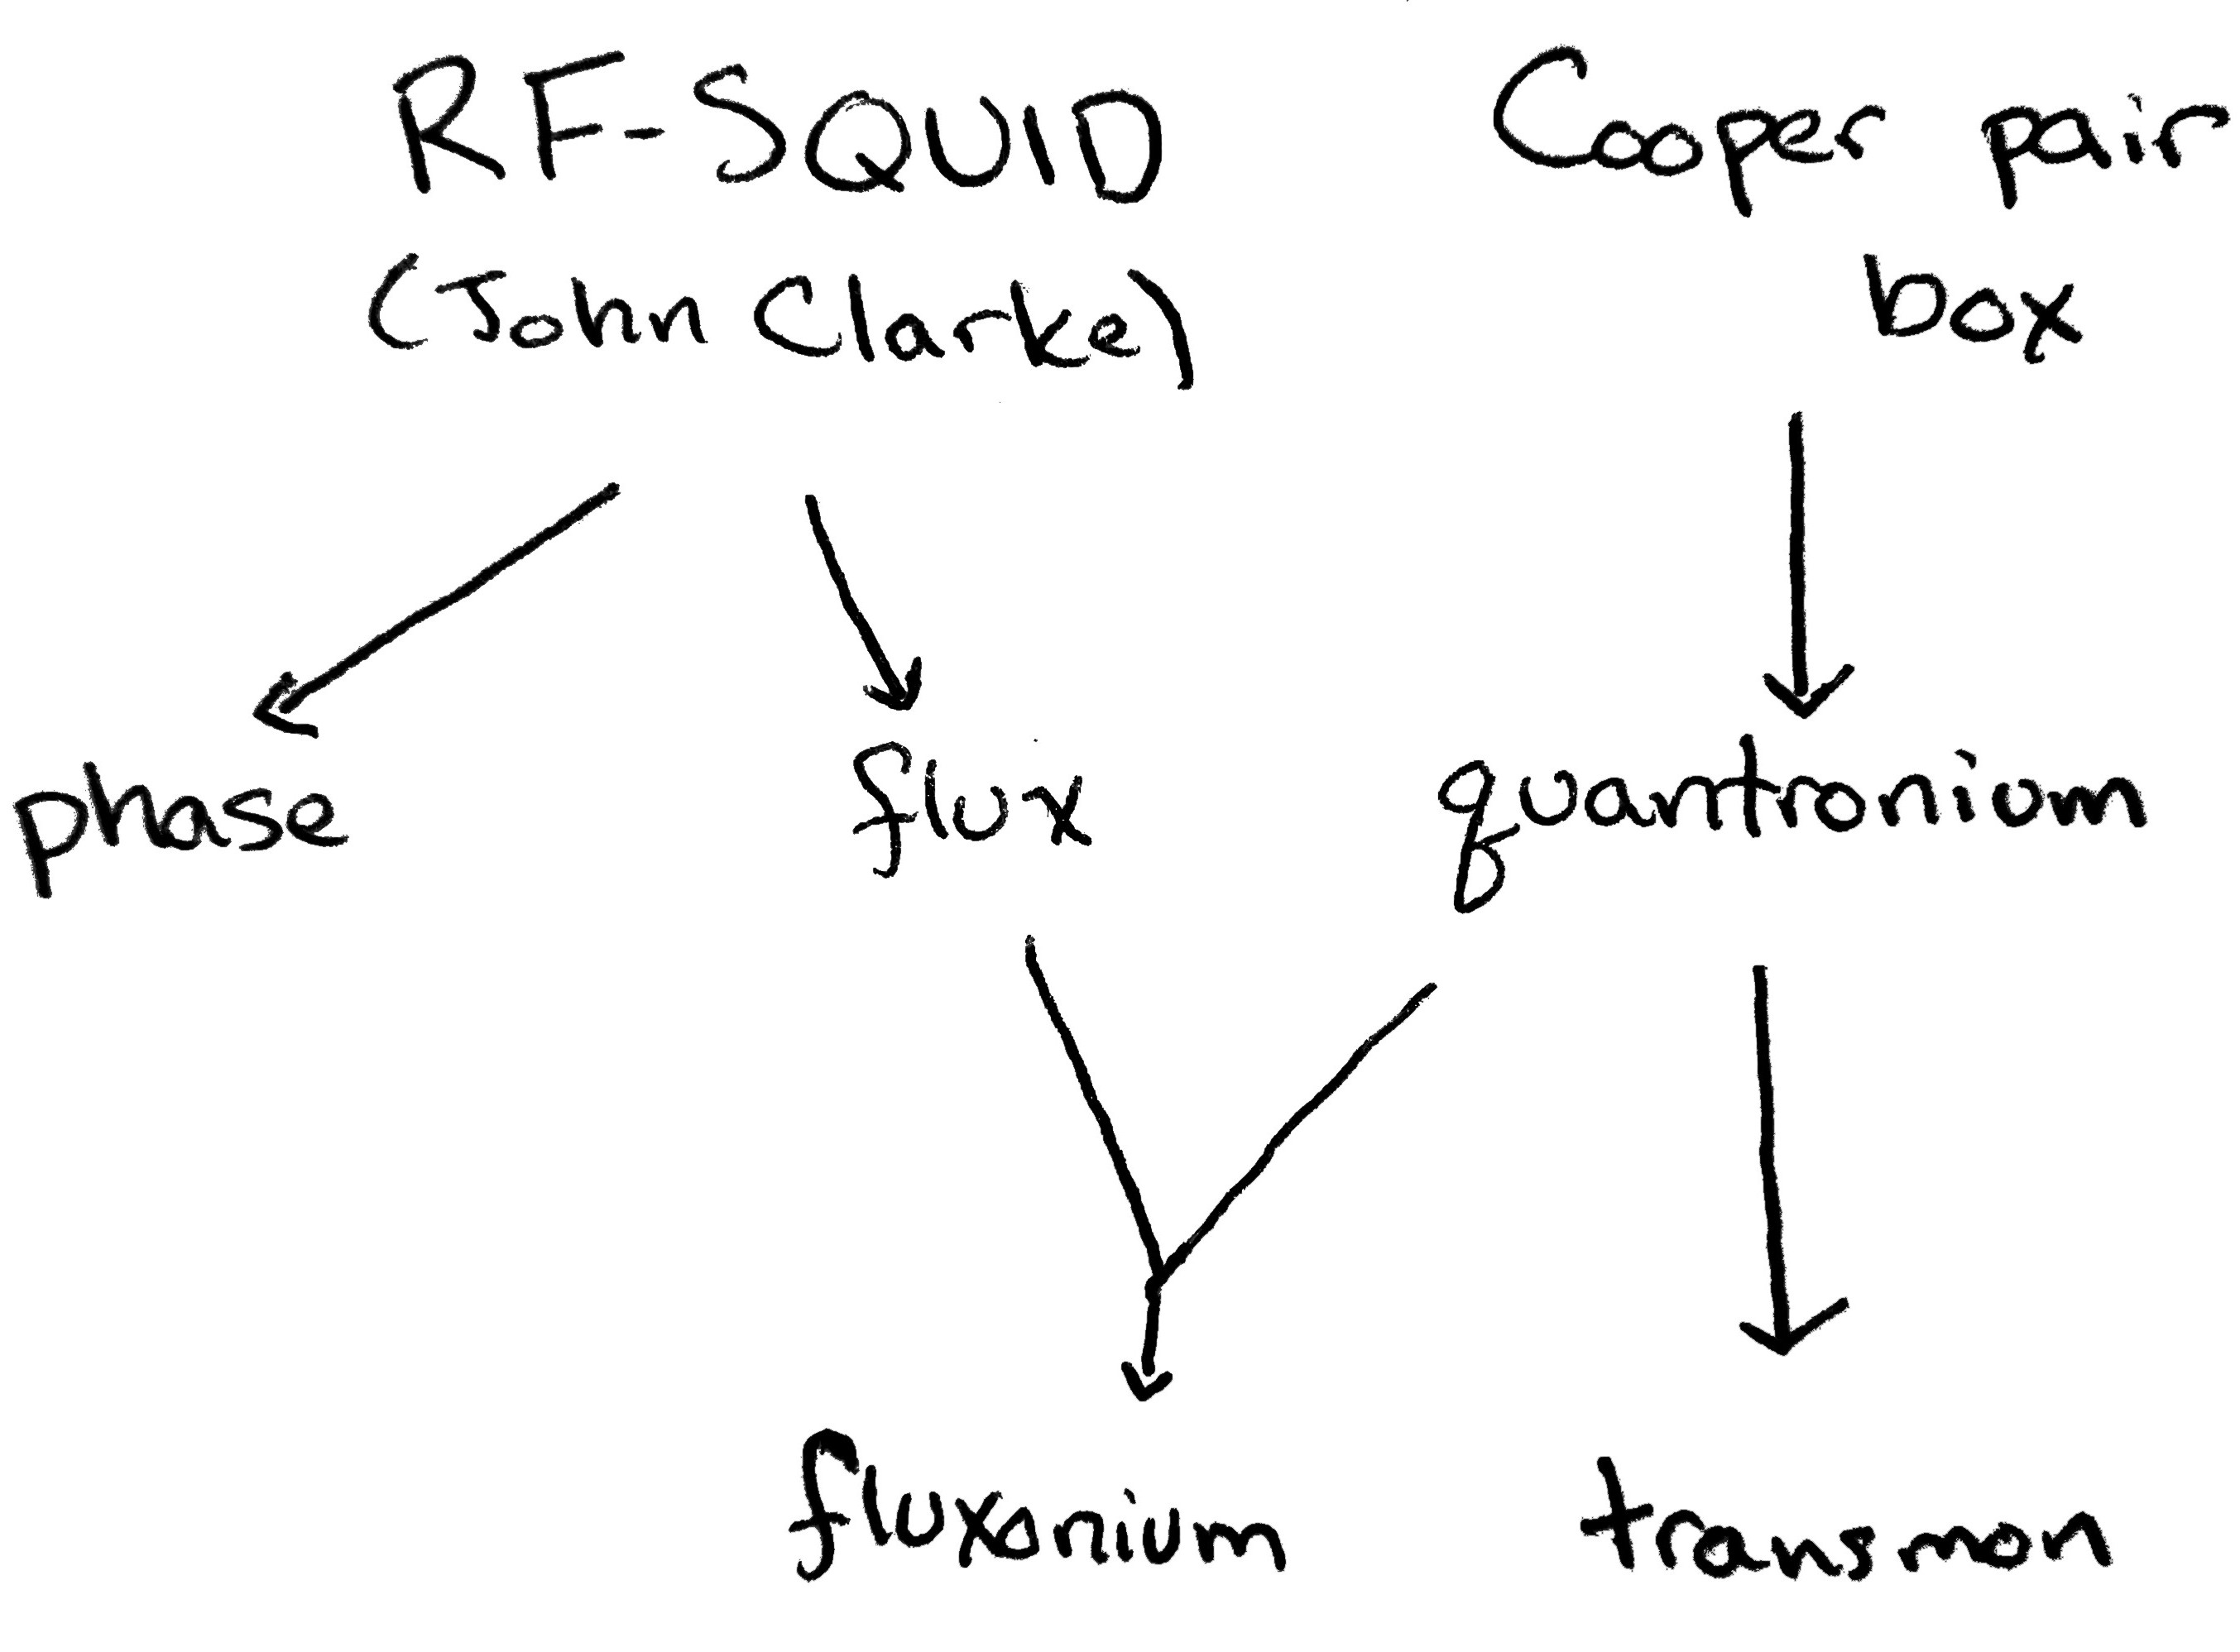
\includegraphics[width=0.7\linewidth]{family-tree.jpg}
    \caption{Family tree of superconducting qubits.}%
    \label{fig:supercond-qubit-family-tree}
\end{figure}

Cooper pair box is topologically distinct from the other designs in that it has
no wire closing the loop around the junction. It consists very simply of a
small antenna whose two halves are connected by a Josphson junction.

$\implies$ Two sides of the junction are not shunted by an inductor.

$\implies$ \# Cooper pairs transferred through the junction is a well-defined
integer. $\comm{Q}{\Phi} = -i\hbar$ $\implies$ periodicity of spectrum in
charge.

$\implies$ charge-based qubits are sensitive to stray electric field noise.

\subsubsection{Lagrangian for a Cooper pair box}
Similar to the LC oscillator except unlike the inductor the energy stored in
the Josephson junctions is not quadratic but periodic.
\[\LL = \frac{1}{2} C_\Sigma \dot{\Phi}^2 + E_J \cos\phi\]
where $\phi$ is phase difference of superconducting order parameter across the
JJ,
\[\phi = 2\pi \frac{\Phi}{\Phi_0} = \frac{2e}{\hbar} \Phi\]
with $\Phi_0 = h/2e$, and $C_\Sigma = C_\text{geometry} + C_J$, thus,
\[\LL = \frac{1}{2} C_\Sigma \left( \frac{h}{2e} \right)^2 \dot{\phi}^2 +
E_J\cos\phi.\]
From Euler-Lagrange,
\[n = \pdv{\LL}{\dot{\phi}} = \frac{\hbar^2}{4e^2} C_\Sigma \dot{\phi}\]
yielding the Hamiltonian,
\[\mathcal{H} = 4E_C(\hat{n} - n_g)^2 - E_J\cos{\phi}\]
where $E_C = e^2/2C_\Sigma$ is charging energy, $n = -i\pdv*{\phi}$ operator,
and $n_g$ is the so-called offset charge representing external bias voltage and
also containing random fluctuations due to stray charges jumping around.

In the limit $E_J \gg E_C$, the low-frequency noise in the offset charge can be
neglected, resulting in very long coherence times $\implies$ ``transmon
qubit.'' With $E_J \gg E_C$ the ``gravitational force'' is very strong, and the
``moment of inertia'' is very large, so the phase angle undergoes very small
quantum fluctuations.
\[H_0 = 4E_C\hat{n}^2 + \frac{E_J}{2} \hat{\phi}^2\]
\[V = E_J\left[-\hat{\phi}^4 / 4! + \cdots\right].\]
We see $H_0$ is the Hamiltonian of a simple LC harmonic oscillator with
frequency $\hbar\Omega = \sqrt{8E_JE_C}$ and with leading order effect of the
JJ being to play the role of a relatively large linear inductor. In the limit
$E_J \gg E_C$, we are effectively ignoring the fact that $\hat{\phi}$ is an
angular variable. It is this assumption which makes conjugate momenta $\hat{n}$
have continuous rather than integer values.


\subsection*{Example}
Q:

 Using the current-phase and voltage-phase relationship of a single Josephson junction: 
\begin{enumerate}[label=(\alph*)]
    \item derive the inductance of a Josephson junction?
    \item can it be zero? How about negative?
    \item calculate the Josephson energy.
    \item Now consider our junction is made out of aluminum leads separated by $d = 1.2 nm$ ( at this thickness the resistivity is $5  k\Omega/ square$) with area A. An ideal junction satisfies: $I_c R_n = \Delta$ where $I_c$ is the supercurrent, $R_n$ is the normal resistance and $\Delta$ is the superconducting gap. What is the resonant frequency of this junction?
    \item Imagine we take thee junction and bias it with 10 micro volt of DC voltage. We then monitor the current with an ideal oscilloscope. What frequency do we detect?

\end{enumerate}


A:

a) 
The Josephson effect describes the supercurrent $I_J$ that flows through the junction according to the classical equations 


\begin{equation}
    I_J=I_csin\delta,
    \label{eq:current}
\end{equation}

\begin{equation}
    V=\frac{\Phi_0}{2\pi} \frac{d\delta}{dt}
    \label{eq:Voltage}
\end{equation}
where $\Phi_0 = \frac{h}{2e}$ is the superconducting flux quantum, $I_c$ is the critical-current parameter of the junction, and $\delta$ and $V$ are respectively the superconducting phase difference and voltage across the junction. The dynamical behavior of these two equations can be understood by first differentiating Eq.~\eqref{eq:current} and replacing $\frac{d\delta}{dt}$ with $V$ according to Eq.\eqref{eq:Voltage}

\begin{equation}
    \frac{dI_J}{dt} = I_ccos\delta\frac{2\pi}{\Phi_0}V.
\end{equation}
With $\frac{dI_J}{dt}$ proportional to V, this equation describes an inductor. By defining a Josephson inductance $L_J$ according to the conventional definition $V = L_J\frac{dI_J}{dt}$, one finds
\begin{equation}
    L_J = \frac{\Phi_0}{2\pi I_ccos\delta}.
    \label{eq:josephson-inductance}
\end{equation}

b) The magnitude of the inductance becomes large as $\delta \rightarrow \frac{\pi}{2}$ or $\frac{3\pi}{2}$, and is negative for $ \frac{\pi}{2}<\delta<\frac{3\pi}{2}$.
But it cannot be zero because $\cos\delta$ is bounded on $[-1, 1]$.

c) The energy stored in the junction is given by
\begin{alignat}{1}
    U_J \newline
    &= \int I_JVdt \\
    &=  \int I_csin\delta \frac{\Phi_0}{2\pi} \frac{d\delta}{dt} dt \\
    &= \frac{I_c \Phi_0}{2\pi} \int_0^\delta sin\delta' d\delta' \\
    &= \frac{I_c \Phi_0}{2\pi} (1-cos\delta)
\end{alignat}

d) The resonant frequency of an LC circuit is
\[\omega_0 = \frac{1}{\sqrt{LC}}\]
where the capacitance $C = \epsilon A/d$ with $d=\SI{1.2}{\nano\meter}$ contact separation, $A$ is the area of the interface between the superconducting aluminum contacts and the insulating medium between them, and $\epsilon$ is the dielectric constant of the insulator.
The inductance $L = L_J$, as given in Eq.~\eqref{eq:josephson-inductance}, depends on the critical current $I_c$, which can be obtained from the product
\[I_cR_n = \Delta \implies I_c = \Delta/R_n\]
where $\Delta$ is the superconducting gap, and the normal resistance of the junction $R_n = \rho d/A$, with $\rho$ the resistivity. Then
\begin{equation}
    \omega_o =\frac{1}{\sqrt{\frac{\Phi_0}{2\pi cos\delta} \frac{\rho\epsilon}{\Delta}}}
\end{equation}

Note there is some ambiguity in the resistivity provided in the problem. Normally, resistivity has units of $[\si{resistance{\cdot}length}]$, whereas the resistivity given in the problem has units of $[\si{resistance{\cdot}length^{-2}}]$. If we assume $\rho = \SI{5}{\kilo\ohm/length^2}$ as given in the problem, and take $R_n = \rho A$, then we obtain
\begin{equation}
    \omega_o =\frac{1}{\sqrt{\frac{\Phi_0}{2\pi cos\delta} \frac{\rho A}{\Delta} \frac{\epsilon A}{d} }}     
\end{equation}

e) The bias voltage introduces a time-dependent phase,
\begin{equation}
    V_{dc} = \frac{\Phi_0}{2\pi} \frac{d\delta}{dt}  \rightarrow \delta = \frac{2\pi V_{dc}}{\Phi_0}t
\end{equation}
Then, by the current-phase relationship of the junction,
\begin{equation}
    I_J = I_c\sin\delta
    = I_c \sin\left(2\pi\frac{V_{dc}}{\Phi_0}t\right) \equiv I_c \sin(2\pi f_0 t)
\end{equation}
which implies a frequency
\begin{equation}
    f_0 = \frac{V_{dc}}{\Phi_0} = \frac{V_{dc}}{\frac{h}{2e}} = \frac{10 \mu V}{\frac{4.135 \times 10^{-15} eVs}{2e}} = \SI{4.8368}{GHz}
\end{equation}










\section{Superdense coding}
Information theory (Shannon): by sending $n$ bits, you cannot
communicate more than $n$ bits of information.

\emph{Superdense coding}: Alice can send Bob 2 \emph{classical} bits by sending
him \emph{only one qubit}. (Catch: A\&B must share some entangled qubit ahead
of time. With no prior entanglement, Alice can't send more than one bit per
qubit.)

\begin{itemize}
    \item Alice: $\ket{\psi} = \alpha\ket{0} + \beta\ket{1}$.
    \item Alice and Bob share a Bell pair in advance:
        $\ket{\Psi^+} = (\ket{00} + \ket{11})/\sqrt{2}$.
    \item  Alice is going to \emph{manipulate} her half, then send her qubit to
        Bob, and Bob can measure both qubits and get 2 bits of information from
        Alice.
\end{itemize}
2 qubits $\rightarrow$ 4 states in basis. Will apply a NOT gate and phase flip.
Alice can find 3 orthogonal states to the original Bell pair; these will be the
other states of the Bell basis \eqref{eq:bell-basis}. Label the two qubits $x$
and $y$.
\begin{itemize}
    \item If $x=1$, she applies a NOT gate.
    \item If $y=1$, she applies a phase gate.
\end{itemize}
For Bob to decode the information, he has to use the inverse transformation.


\section{Density matrices}
\footnote{10/28/19}(This is from Scott Aaronson's Quantum Computation course \cite[Lec. 6]{scaaronson}.) So far Basis
states are defined: $\{\ket{0}, \ket{1}\} \rightarrow \ket{i}$. Pure states are
superpositions of basis states: $\ket{\psi} = \sum\alpha_i \ket{i}$. Pure
states exist in isolated quantum systems but you can also have quantum
superposition layered together with regular, old probabilistic uncertainty. In
some sense, mixed states are a distribution over quantum states, so
\[\{P_i, \Psi_i\} = P_1\ket{\Psi_1}, \ldots, P_n\ket{\Psi_n},\]
meaning that with probability $P_i$ the superposition is $\ket{\Psi_i}$. Mixed
states (that is, the components $\ketbra{\psi_i}$ of the mixed state) don't
have to be orthogonal. Pure state is a degenerate case of a mixed state where
all the probabilities are 0, except for one $P_i$ which is 1.

We write a mixed state as a \emph{density matrix}:
\[\rho = \sum_i = p_i\ketbra{\psi_i}.\]
(Examples of outer product in matrix representation.)

For any two orthgonal states $\ket{v}$ and $\ket{w}$,
\[\frac{\ketbra{v} + \ketbra{w}}{2}  = \frac{\id}{2}\]

Measuring $\rho$ in the basis $\ket{1}, \ldots, \ket{N}$ gives outcome
$\ket{i}$ with probability $\Pr\left(\ket{i}\right) = \rho_{ii} =
\ev{\rho}{i}$. A diagonal density matrix is another way of writing a classical
probability distribution, e.g. $\pmqty{\dmat[0]{P_1,P_2}}$.

Rank of a matrix: $\rank(\rho) =$ the number of non-zero eigenvalues. The rank
of an $n\times n$ matrix is at most $n$.

The matrix $\id/2$ is the even mixture of $\ket{0}$ and $\ket{1}$. It is also
an even mixture of $\ket{+}$ and $\ket{-}$. This is a \emph{maximally mixed
state}. If we do a unitary transformation $U$ on the states $\ket{\psi_i}$
comprising $\rho$,
\[\rho' = \sum_i P_i \left(U\ket{\psi_i}\right)\left(U\ket{\psi_i}\right)^\dag
= \sum_i P_i U\ketbra{\psi_i}U^\dag = U\rho U^\dag\]
i.e. the new density matrix is unitarily transformed. E.g. $\ketbra{+} =
\pmqty{\xmat{\frac{1}{2}}{2}{2}}$ in the $\{\ket{0}, \ket{1}\}$ basis, and the
off-diagonals represent the
interference between $\ket{0}$ and $\ket{1}$.

What are the constraints on $\rho$?
\begin{itemize}
    \item Square $n\times n$.
    \item Hermitian $\rho^\dag = \rho$.
    \item Probability $\sum_i \rho_{ii} = 1 = \Tr{\rho}$.
    \item Positive semidefinite: all eigenvalues are nonnegative (since they
        represent probabilities).
\end{itemize}

(Examples of pure vs. mixed states.)

Alice and Bob may share a bipartite state described by a density matrix. The
state of each's qubit is described by the reduced density matrix obtained by
taking a partial trace over the other's qubit space. The key points:
\begin{itemize}
    \item A density matrix encodes all and only what is physically observable.
    \item Two quantum states will lead to different probabilities iff they have
        different density matrices.
    \item No communication theorem: If Alice and Bob share an entangled state,
        nothing $A$ chooses to do will have any effect on Bob's density matrix
        $\implies$ there is no observable effect on Bob's end.
\end{itemize}

Basis state $\ket{i}$. Pure state $\ket{\psi} = \sum_i \alpha_i \ket{i}$. Mixed
state $\{P_i, \ket{\psi_i}\} \rightarrow \rho = \sum_i P_i \ketbra{\psi_i}$,
classical probability distributions over pure states.

What represents better the actual physical reality? Pure vs. mixed? When we
look at part of an entangled state, a mixed state is the most complete
representation possible that only describes the part that we are looking at.


\section{Quantifying entanglement}
\footnote{10/30/19}How do you quantify how much entanglement there is between
two quantum systems? $\leftrightarrow$ measuring entanglement.

Entanglement is our resource $\leftrightarrow$ EPR $(\ket{00} +
\ket{11})/\sqrt{2}$. Entanglement of pure states; entanglement of mixed states.

\subsection{Schmidt decomposition}
Given $\sum_{ij}\alpha_{ij}\ket{i}_A\ket{j}_B$, how do we calculate how many
EPR pairs it's worth?

Let $A = \pmqty{\alpha_{ij}}$. In bipartite states, we can always find a change
of basis on Alice's side and another on Bob's side that puts the state into the
simpler form (Schmidt decomposition) $\sum_i \lambda_i \ket{v_i}\ket{w_i}$
where $\{\ket{v_i}\}$ is an orthonormal set, and $\{\ket{w_i}\}$ is an
orthonormal set. This follows from the singular value decomposition of the
matrix $A$: we can multiply $A$ by two unitary matrices, one on each side, to
get a diagonal matrix $\Lambda = UAV$. Measuring in the $\{\ket{v_i},
\ket{w_i}\}$ basis would then yield the probability distribution
\begin{equation}
    \pmqty{\abs{\lambda_1}^2, \ldots, \abs{\lambda_2}^2}^T.
    \label{eq:probability-distribution}
\end{equation}

\subsection{Entropies}
\subsubsection{Shannon entropy}
For classical probability distribution $D = (P_1, \ldots, P_n)$, the Shannon
entropy is
\[H(D) = \sum_{i=1}^n P_i\log_2\frac{1}{P_i} = -\sum_{i=1}^n P_i\log_2 P_i\]
E.g.
\begin{itemize}
    \item  $D = (0, 1) \implies H(D) = -0\log_20 - 1\log_21 = 0$.
    \item $D = (\frac{1}{2}, \frac{1}{2}) \implies H(D)
        -2(\frac{1}{2}\log_2\frac{1}{2}) = 1$
\end{itemize}
For the distribution \eqref{eq:probability-distribution}, we can calculate the
ordinary Shannon entropy of our system as
\[\sum_i\abs{\lambda_i}^2\log\frac{1}{\abs{\lambda_i}^2}\]
in order to figure out how many Bell pairs our state is equivalent to.

\subsubsection{Von Neumann entropy}
Generalizes Shannon entropy from classical probability distributions to quantum
mixed states. We say that the von Neumann entropy of a mixed state $\rho$ is
\[S(\rho) = \sum_{i=1}^N \lambda_i \log_2 \frac{1}{\lambda_i}
= -\sum_i \lambda_i \log_2\lambda_i.\]
The von Neumann entropy is the Shannon entropy of the vector of eigenvalues of
the density matrix of $\rho$ (i.e. $\lambda_i$'s here are probabilities).

The von Neumann entropy of any pure state $\ketbra{\psi}$ is zero because there
is always some measurement basis that returns a definite outcome (i.e. the
basis containing $\ket{\psi_i}$). Example: you could measure $\ket{+}$ in the
$\{\ket{0}, \ket{1}\}$ basis where you have complete uncertainty and Shannon
entropy of 1, but if you measure in the $\{\ket{+}, \ket{-}\}$ basis you have
complete certainty with Shannon entropy of 0. In either case, the von Neumann
entropy is 0.

Von Neumann entropy of a maximally mixed qubit state $\id/2$ is 1. The von
Neumann entropy of a maximally mixed $n$-qubit state $\id/2^n$ is $n$.

Suppose Alice and Bob share a bipartite pure state $\ket{\psi} =
\sum_{ij}\alpha_{ij}\ket{i}_A\ket{j}_B$. To quantify the entanglement entropy,
we trace out either Alice or Bob's part of the system and calculate the von
Neumann entropy of the reduced density matrix representing just Bob's are
Alice's part, respectively (which we choose should not matter, $S(\rho_A) =
S(\rho_B) = H(\lambda_i)$, Shannon entropy of $\lambda_i$ which you get by
diagonalizing the Alice's or Bob's reduced density matrix.


\section{Mixed vs. pure states}
\footnote{11/4/19}Diagonal elements $\rho_{ii}$ of a density matrix represent
the populations in the chosen basis:
\[\rho = \sum_i p_i \ketbra{i}, \qquad \ket{i} = \sum_p c_p^{(i)}\ket{p}\]
\[\rho_{ii} = \sum_p = \abs{c_p^{(i)}}^2p_i \rightarrow
\text{population in state $\ket{i}$}\]
The off-diagonal elements $\rho_{ij}$ of a density matrix provide information
on interference of $\ket{i}$ and $\ket{j}$ $\rightarrow$ they represent
coherence in mixed states. When a qubit is coupled to an environment, this
coupling can cause time-dependence of elements of density matrix $\rightarrow$
Decay of the off-diagonal elements is referred to as ``dephasing'' ($T_2$)
while the decay of the diagonal elements is referred to as ``relaxation'' or
``dissipation'' ($T_1$).

What is the difference between the pure state $\frac{1}{\sqrt{2}}(\ket{0} +
\ket{1}) = \ket{+}$ and mixed state $\frac{1}{2}(\ketbra{0} + \ketbra{1}) =
\id/2$? Let's apply a Hadamard gate to both:
\begin{align}
    &\text{pure state} & H\ket{+} &= \ket{0} \\
    &\text{mixed state} & H\id H/2 &= \id/2
\end{align}
In the first case the amplitudes can interfere and produce $\ket{0}$ while in
the second case the states cannot interfere because they are in an
``incoherent'' mixture of the two states.

Open quantum systems can produce evolution which starts out in a pure state and
evolves into a mixed state $\rightarrow$ such evolution can destroy our quantum
computation $\rightarrow$ quantum error correction.

Recall,
\[\rho = \pmqty{\dmat{\rho_{11},\rho_{22},\ddots,\rho_{nn}}}, \qquad
\Tr\rho = \sum_i \rho_{ii} = 1\]
A nice property of the trace operation is that a basis change leaves it
invariant. Trace has a cyclical property,
\[\Tr(ABC) = \Tr(BCA) = \Tr(CAB).\]
Expectation value of any operator $\hat{O}$ in terms of projectors
$\hat{P}_\psi$ can be given by:
\[\ev{\hat{O}}_\psi = \ev{\hat{O}}{\psi} = \Tr(\hat{O}\hat{P}_\psi)
=  \Tr(\hat{P}_\psi\hat{O}).\]
Suppose we take pure states $\ket{\pm}$. The density matrices are
\[\rho_\pm = \frac{1}{2}\pmqty{1&\pm1\\\pm1&1},\]
while the classical mixture is
\[\rho = \sum_{i=\pm} p_i\ketbra{i} = \sum_{i=\pm} p_i \rho_i,\]

Statistical physics: statistical mixture of energy eigenstates in thermal
equilibrium:
\[\rho = \sum_np_n\ketbra{n}, \qq{where}
p_n = \frac{e^{-E_n/kT}}{\mathcal{Z}}, \qq{and}
\mathcal{Z} = \sum_ne^{-E_n/kT}.\]
$\mathcal{Z}$ is the partition function. When the Hamiltonian does not depend
on time, the mixture is time-independent.

Example: mixture where we prepare $\ket{0}$ with probability $\frac{1}{2}$ and
$\ket{+}$ with probability $\frac{1}{2}$.
\[\rho = \frac{1}{2}\pmqty{1&0\\0&0}
+ \frac{1}{2}\pmqty{\frac{1}{2}&\frac{1}{2}\\\frac{1}{2}&\frac{1}{2}}
= \frac{1}{4}\pmqty{3&1\\1&1}\]
The eigenvalues are $\lambda_\pm = \frac{1}{2} \pm \frac{\sqrt{2}}{4}$, with
eigenvectors $\ket{\phi_\pm} = \sqrt{\lambda_\pm}\ket{0} +
\sqrt{1-\lambda_\pm}\ket{1}$. We can now view the mixed state as a mixture of
two eigenstates $\ket{\phi_\pm}$ with weights equal to $\lambda_\pm$.

There are two simple ways to determine whether $\rho$ describes a pure state
or not:
\begin{enumerate}
    \item Pure state $\Leftrightarrow$ $\rho^2 = \rho$.
        Mixed state $\Leftrightarrow$ $\rho^2 \neq \rho$.
    \item Pure state $\Leftrightarrow$ $\Tr\rho^2 = 1$.
        Mixed state $\Leftrightarrow$ $\Tr\rho^2 < 1$.
\end{enumerate}
In fact, we can define the ``purity of a state'' $P \equiv \Tr\rho^2$. A state
is pure if $P=1$ and mixed otherwise. Example: $n$ qubits, dimension $d = 2^n$
$\rightarrow \rho = \id/d$,
\[\implies P = \Tr((\id/d)^2) = \sum_{1}^d \frac{1}{d^2} = \frac{1}{d}.\]
Entropy $S(\rho) = -\sum_k \lambda_k\log_2\lambda_k$ (note $\lim_{x\rightarrow
0} x\log x = 0$). We use log base 2 so that the unit of the entropy is the
``bit.'' We can interpret the entropy as the missing information (in bits)
about the state. Pure state: $S(\rho) = 0$. Mixed state: $S(\rho) > 0$.

\subsection{Reduced density matrix}
Consider a measurement just on system A, say of an observable $O_A$. The
expectation value of that observable in terms of $\rho_{AB}$ is
\begin{align}
    \ev{O_A} = \Tr(\rho_{AB}O_A) &= \sum_{nm} \ev{\rho_{AB}O_A}{n_Am_B} \\
    &= \sum_{nm} \ev{\ev{\rho_{AB}}{m_B}O_A}{n_A}.
\end{align}
We then define the reduced density matrix for A as a partial trace over B,
\[\rho_A = \sum_m \ev{\rho_{AB}}{m} \equiv \Tr_B\rho_{AB},\]
and then any observable in A can be expressed,
\[\ev{O_A} = \Tr(\rho_AO_A).\]
That is, $\rho_A$ describes the state of system A alone.

\subsection{Quantifying entanglement in mixed states}
\footnote{11/6/19}(See \cite[Lec. 11]{scaaronson}.) For
bipartite mixed state there are two entanglement measures to consider:
\begin{itemize}
    \item \emph{Entanglement of formation:} $E_F(\rho_{AB})$ is the
        number of entangled qubits that A and B need to create one copy of the
        state $\rho_{AB}$ (in the limit where they are creating many copies of
        it, and assuming they are allowed unlimited local operations and
        classical communication (LOCC) for free).
    \item \emph{Distillable entanglement:} $E_D(\rho_{AB})$ is the number of
        entangled qubits that A and B can extract per copy of $\rho_{AB}$ again
        in LOCC for free.
\end{itemize}
Clearly $E_F \geq E_D$ since if you could ever get out more entanlgment than
you put it, it would give you a way to increase entanglement (entropy)
arbitrarily using LOCC, which is impossible.

What about $E_F \gg E_D$? There exist bipartite states that take a lot of
entanglement to make but you can only extract a small fraction of the
entanglement.

A bipartite state $\rho_{AB}$ is separable if there is a way to write it as a
mixture of product states:
\[\rho_{AB} = \sum_ip_i\ketbra{v_i}\otimes\ketbra{w_i}\]
A mixed state is called entangled iff it is \emph{not} separable. It could
happen that a density matrix looks entangled \emph{but} there's some
decomposition that shows it is separable.

Proven by Leonid Gurvits, 2003: If you are given a density matrix $\rho_{AB}$
for a bipartite state then deciding whether $\rho_{AB}$ represents a separable
or entangled state is an NP-hard problem.


\section{Some standard results, protocols, and other bits and bobs}
\subsection{No-cloning theorem}
Assume that $U$ is a unitary transformation that clones in that $U\ket{a0} =
\ket{aa}$ for all quantum states $\ket{a}$. Let $\ket{a}$ and $\ket{b}$ be
orthogonal quantum states. Clearly $U\ket{a0} = \ket{aa}$ and $\ket{b0} =
\ket{bb}$. But consider a superposition state, $\ket{c} = (\ket{a} +
\ket{b})/\sqrt{2}$:
\[U\ket{c} = \frac{1}{\sqrt{2}}(\ket{aa} + \ket{bb}) \neq \ket{cc},\]
therefore $U$ is not a cloning operation.

It is possible to clone a known quantum state. The no-cloning theorem says we
cannot reliably clone an \emph{unknown} state. Nor is cloning possible by using
measurements.

\subsection{Quantum teleportation}
It is possible for Alice and Bob to use pre-shared entanglement plus classical
communication to perfectly transmit a qubit.

Alice has a single qubit $\ket{\psi} = \alpha\ket{0} + \beta\ket{1}$. She also
shares the EPR pair $(\ket{00} + \ket{11})/\sqrt{2}$. Alice applies some
transformation to $\ket{\psi}$ that entangles it with her half of the Bell
pair. She then measures her qubit. Alice tells Bob the measurement outcomes
over the phone. Bob then applies some transformation to his qubit of the
entangled pair and ``magically'' will have $\ket{\psi}$.

(Example.) Alice applies CNOT with $\ket{\psi}$ as control and her half of the
Bell state as target. Alice then applies Hadamard on $\ket{\psi}$. Alice
measures both of her qubits. She tells Bob the result. Depending on the result,
Bob applies a corresponding retrieval transformation on his qubit (which was
part of the Bell pair), which deterministically reproduces $\ket{\psi}$ on
Bob's end. $\implies$ they have transmitted a qubit without a quantum channel.

\footnote{11/11/19}Are we sending infinitely more information than two
classical bits if we can send over enough information to perfectly describe an
arbitrary qubit? In some sense we are sending a perfect qubit but Bob only
obtains the information that he can measure which is significantly less.

We didn't make any assumption that $\ket{\psi}$ has to be unentangled from the
rest of the world. You can have a protocol that has $\ket{\psi}$ to be half of
another Bell pair. This protocol would entangle the 4th qubit to Bob's qubit.
This suggests that it should be possible to teleport an arbitrary $n$-qubit
entangled state by simply teleporting the qubits one at a time.

A consequence of this is that two qubits don't need to interact directly to
become entangled.  Consider a quantum circuit where $H$ acts on qubit 1,
followed by a CNOT acting on qubit 2 conditioned on 1, followed by a SWAP gate
between 2 and 3. Qubits 1 and 3 end up entangled even though there's never any
``direct'' contact between them $\rightarrow$ SWAP gate.  \emph{Entanglement
swapping:} If Alice has two entangled qubits and also two EPR/Bell states
shared with Bob, she can teleport both of her qubits to Bob whereupon they will
be entangled on Bob's end, even though the two qubits on Bob's end were never
in causal contact with each other.

\subsection{GHZ states}
There is a 3-qubit analogue of the Bell pair called a \emph{GHZ state:}
\begin{equation}
    \frac{\ket{000} \ket{111}}{\sqrt{2}}
    \label{eq:GHZ-state}
\end{equation}
Suppose three players share a GHZ state, where all three can see the state is
entangled. What if Charlie is gone? Can Alice and Bob still see they are
entangled? No. Charlie could have measured his qubit without Alice and Bob
knowing. But if he did then Alice and Bob would have classical correlation
only: either both 0s if Charlie measured zero or 1s if he measured one.
Regardless of whether Charlie measured or not, A and B cannot know if they are
entangled. (Like Borromean rings.)

\subsection{CHSH game}
\subsubsection{Classical version}
We put Alice and Bob in separate rooms and each are given a challenge bit ($x$
and $y$ respectively) by a referee. The challenge bits are chosen uniformly at
random and independently of each other. Then Alice sends an answer bit $a$ back
to the referee and Bob sends back bit $b$. Alice and Bob win the game if
\[a + b = xy\mod{2} \Longleftrightarrow\
\begin{cases}
    a = b &\text{if $x=0$ or $y=0$}\\
    a \neq b &\text{if $x=y=1$}
\end{cases}\]
Alice and Bob know the rules and are allowed to strategize together beforehand.

\textbf{Optimal strategy:} Alice and Bob always return $a=0$ and $b=0$. They
win with probability 3/4. (They win on $(x,y) \in \{(0,0),(0,1),(1,0)\}$ and
lose on $(x,y)=(1,1)$.)

\subsubsection{Quantum version}
If Alice and Bob can share a Bell pair, they can win with probability
$\cos^2\frac{\pi}{8} \approx 85\%$

\footnote{11/13/19}\fbox{App.~\ref{sec:quinfo}.}

\footnote{11/18/19--11/20/19}\fbox{Mid-project presentations.}

\footnote{11/25/19}The strategy involves A and B measureing their respective
qubits in \emph{different bases} depending on whether their input bits $x$ and
$y$ are 0 or 1, and then outputting bits $a$ and $b$ respectively based on the
outcomes of those measurements. Let's consider the case where A gets $x=0$ and
she measures $\ket{0}$, she will output $a=0$ and A and B will win iff Bob
outputs $b=0$. Given that A measured her qubit already Bob's qubit has
collapsed to the state $\ket{0}$. First suppose $y=0$. Bob measures $\ket{0}$
in a basis rotated by $\pi/8$. He outputs 0 and they win. Probability of Bob
outputting zero is $\cos[2](\frac{\pi}{8}) \approx 85\%$.

\subsubsection{Einstein-certified randomness}
In crypto, one of the most important tasks is to create random numbers.
\[\ket\psi = a \ket 0 + b \ket 1 \Longleftrightarrow n \text{ assumptions}\]
Once we have quantum mechanics, you might think that the solution is trivial.
After all, you get a random number by measuring the $\ket +$ state in the
computational basis. For cryptography, though, this is insufficient. The Bell
inequality lets us certify numbers as being truly random under very weak
assumptions, namely, that information cannot travel faster than the speed of
light.

Given a black box device that generates random numbers, we use one to generate
a bit $x$ and another to generate a bit $y$, and then just play the CHSH game.
If the win probability is $\cos[2](\frac{\pi}{8})$, it's perfectly random.
Anything above 3/4 is certifiably random to some degree. Now suppose you have
two boxes, designed by your enemies, that share quantum entanglement. Referee
sends random $x,y$, boxes return $a,b$. Play CHSH game: if $\Pr$(success) =
$\cos[2](\frac{\pi}{8})$, we declare the string truly random.

Shannon entropy: $\displaystyle \sum p_x \log_2 \frac{1}{p_x}$ where $p_x$ is
the probability that string $x$ will be in general less than $n$. Problem: we
need the input bits to be uniformly random in order to play CHSH game. I.e.
$x,y$ truly random, $a,b$ not truly random.

Pironio et al.: You don't have to give Alice and Bob perfectly random
bits every time. Instead, you can input $x=y=0$ most of the time, and
occasionally input some random $x$'s and $y$'s to prevent Alice and Bob
from figuring out the pattern. This is because Alice and Bob have no
way of knowing whether each round is for testing or randomness
generation.

How much entropy can we get out per bit of entropy put in?
\begin{itemize}
    \item Colbeck et al.: You can get $cn$ bits out per $n$ bits in ($c
        > 1$).
    \item Pironio et al.: $n^2$.
    \item Vazirani et al.: $\exp(\sqrt{n})$.
\end{itemize}
How many random numbers do I need to jump start this? One naive way is
to feed Alice and Bob the same true random bits that they themselves
create $\rightarrow$ it is not random to them. Doesn't work.
\begin{itemize}
    \item Courdon \& Yuan: Suppose we only have a fixed number of A and
        B players. (e.g. suppose $A,B \rightarrow$ referee $\rightarrow
        C,D$).
    \item Aaronson \& Gross: Few tens of thousands (upper bound).
\end{itemize}
Reichardt et al. (2012): As long as we have two quantum computers, and as long
as they are entangled with each other but unable to exchange messages, we can
use CHSH game to \emph{verify} that the computers are behaving as expected.


\section{Computational complexity}
\footnote{12/2/19}The study of how many resources are required to solve various
problems. Divide problems into ``easy'' and ``hard.''  Easy problems are those
for which the resources needed to solve them grow only like some polynomial in
input size. E.g. multiplication of $n$-bit integer $\rightarrow$ add \& shift
$\rightarrow$ $n \times 2n$ bitwise addition, which we say is
$\mathcal{O}(n^2)$.

Now consider factoring $n$-bit number, $x$. The simplest algorithm is to check
all the numbers up to $\sqrt{x}$. This requires $2^{n/2}$ checks $\rightarrow$
exponentially difficult in $n$ $\implies$ hard.
\[n \rightarrow \begin{cases}
    \text{factoring} & 2^{n/2} \rightarrow \text{hard}\\
    \text{multiplication} & n^2 \rightarrow \text{easy}
\end{cases}\]

\subsection{Complexity classes}
\begin{figure}[htpb]
    \centering
    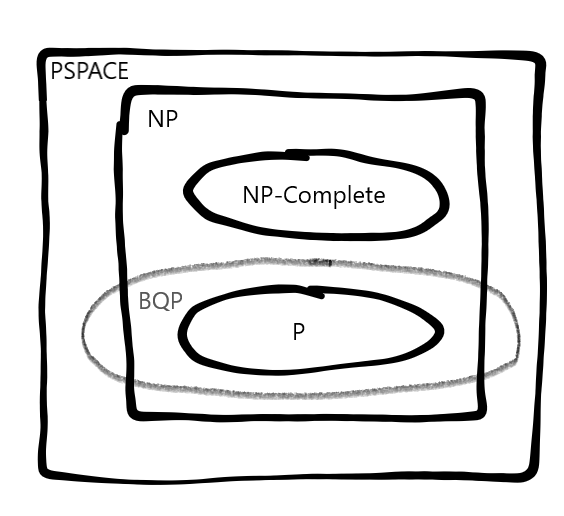
\includegraphics[width=0.5\linewidth]{complexity.png}
    \caption{Potential relationship between the complexity classes.}%
    \label{fig:complexity}
\end{figure}
See Fig.~\ref{fig:complexity}.
\begin{itemize}
    \item P (polynomial time): Class of decision problems which we can
        solve in polynomial time ($\implies$ polynomial memory).
    \item NP (nondeterministic polynomial): Class of problems which we
        \emph{may} not be able to solve but we can \emph{verify} a solution in
        polynomial time (and $\therefore$ polynomial memory) if it is given to
        us. $P \subseteq NP$.
    \item NP-hard: Problems which are at least as hard as \emph{anything} in
        NP. That is, if someone were to give you a box that efficiently solved
        an NP-hard problem, you could use it to solve any problem in NP in
        polynomial time.
    \item NP-complete: Problems which are both NP-hard and are themselves in
        NP.
    \item NP-intermediate: Problems which are in NP but are not in P or in
        NP-complete.
    \item BQP (bounded-error quanutm polynomial): Class of decision problems
        solvable in polynomial time on a quantum computer with a probability of
        error less than 1/3. It seems BQP overlaps with NP-intermediate (e.g.
        Shor's algorithm).
    \item PSPACE (polynomial space): Class of problems solvable using
        polynomial memory but perhaps requiring exponential time.
\end{itemize}

\subsection{3-SAT}
\newcommand*\AND{\wedge}
\newcommand*\OR{\vee}
\newcommand*\NOT[1]{\overline{#1}}
See Ref.~\citenum{plank}.

3-SAT is a very simple NP-complete problem. We are given a boolean epression
which is a big AND ($\AND$) of clauses,
\[E = C_0 \AND C_1 \AND \cdots \AND C_{m-1},\]
where each clause $C_i$ is an OR ($\OR$) of three literals,
\[E = \underbrace{(a \OR b \OR c)}_{C_0} \AND \underbrace{(\NOT a \OR \NOT b
\OR \NOT c)}_{C_1} \AND \underbrace{(a \OR \NOT b \OR \NOT c)}_{C_2} \cdots \]
Is there an assignment of the variables so that $E$ is true?

Independent set decision problem (ISDP): Given a graph $G$
and a number $k$, can we find a set of $k$ vertices in $G$ such that there are
no edges between any two of the vertices? We want to use 3-SAT to prove that
ISDP is NP-complete. First note if you are given a set of $k$ vertices you can
easily check to verify that there are no edges between two nodes in the set.
Second, map 3-SAT to ISDP:
\begin{enumerate}
    \item Turn each clause into 3 nodes and label the nodes with their
        literals.
    \item For every pair of nodes with the same, but negated literals (e.g. $b$
        and $\NOT b$), add an edge between that pair of nodes.
    \item Any independent set of size $k$ (corresponding to the number of
        clauses in the 3-SAT expression) will correspond to an assignment of
        the literals for which the 3-SAT expression is true.
\end{enumerate}

\begin{appendices}
\section{Python \& Qiskit: Installation \& Introduction}%
\label{sec:python}
To get started with Python and Qiskit, have a look at Ref.~\citenum{shabani}.

%\section{Guest lecture: Quantum hardware}%
%\label{sec:quantum-hardware}
%Guest lecture by Pat Grumann, IBM.

%\section{Guest lecture: Programming with qiskit}%
%\label{sec:qiskit}
%Guest lecture by Abraham Asfaw, IBM.

\section{Guest lecture: Quantum algorithms}%
\label{sec:quinfo}
Guest lecture by Ali Javadi, IBM.

The hidden shift problem, also known as Simon's problem, is a member of a broader class of so-called ``hidden subgroup'' problems. Given a function $f$ defined over all binary strings of length $n$ such that
\[f(x) = f(x \oplus s) \quad \forall x,\]
where $\oplus$ denotes bitwise addition, the challenge is to find the value of the bitstring $s$, known as the ``hidden shift.'' While the function $f$ is unknown, you are provided with an oracle that can evaluate $f$. In other words, you can ask the oracle the value of $f(x)$ for any $x$.

Classically, this problem requires $\mathcal{O}(2^{n/2})$ queries to the oracle in order to deduce $s$ with high probability.  Using a quantum algorithm (such as Simon's algorithm), this problem may be solved in $\mathcal{O}(n)$ queries, an exponential speedup.

Ref.~\citenum{javadi} demonstrates how to solve for the hidden shift of a ``bent'' function in Qiskit.

\section{Additional Problems}
%%%%%% ------------------------- Q1
\subsection*{Q1}

Any measurement performed in qiskit is always done along the z-axis of the Bloch sphere, it is however not always the relevant axis in practice. Using adequate operation on the qubit before the measurement, can you figure out how deduce the projection of the qubit state on all three axis of the Bloch Sphere (x, y, z) ? 

The answer should rely on the use of the qasm simulator which reflects the actual behavior of the quantum hardware. However feel free to use the state vector simulator to figure out the impact of operations on the qubit.

\subsection*{Solution}



It is possible to measure the qubit in any of the three axes of the Bloch sphere by performing a rotation or change of basis right before the measurement. First, the matrix for the change of basis from the $\sigma_z$ basis to the $\sigma_x$ basis is the Hadamard gate:


$$ U(\sigma_z \to \sigma_x) =\frac{1}{\sqrt{2}}\begin{pmatrix}
1&1\\
1&-1\\
\end{pmatrix}.$$
The matrix of change of basis from the $\sigma_z$ basis to the $\sigma_y$ one is:

$$ U(\sigma_z \to \sigma_y) =\frac{1}{\sqrt{2}}\begin{pmatrix}
1&-i\\
1&i\\
\end{pmatrix}.$$

We want to prove that is the case using Qiskit. To do so we need a quantum circuit that firstly takes the initial quantum state $|0\rangle$ and puts it in any desired state $|\psi\rangle = \cos(\theta /2)|0\rangle + e^{i\phi}\sin(\theta /2)|1\rangle$, then performs either rotation $ U(\sigma_z \to \sigma_x)$ or $ U(\sigma_z \to \sigma_y)$ and then performs a measurement. To perform both the state preparation and then the rotation we will use the physical gate:

$$ U_3(\alpha, \beta, \lambda) =\begin{pmatrix}
\cos(\alpha/2)&e^{-i\lambda}\sin(\alpha/2)\\
e^{i\beta}\sin(\alpha/2)&e^{i(\lambda+\beta)}\cos(\alpha/2)\\
\end{pmatrix}.$$

In this language the state preparation is done by applying $U_3(\alpha = \theta, \beta = \phi, \lambda = 0)$ and the rotations as: $ U(\sigma_z \to \sigma_x) =U_3(\alpha = -\pi/2, \beta = \pi, \lambda = 0)$ and $ U(\sigma_z \to \sigma_y) =U_3(\alpha = \pi/2, \beta = 0, \lambda = \pi/2)$: 

    \begin{figure*}[h]
        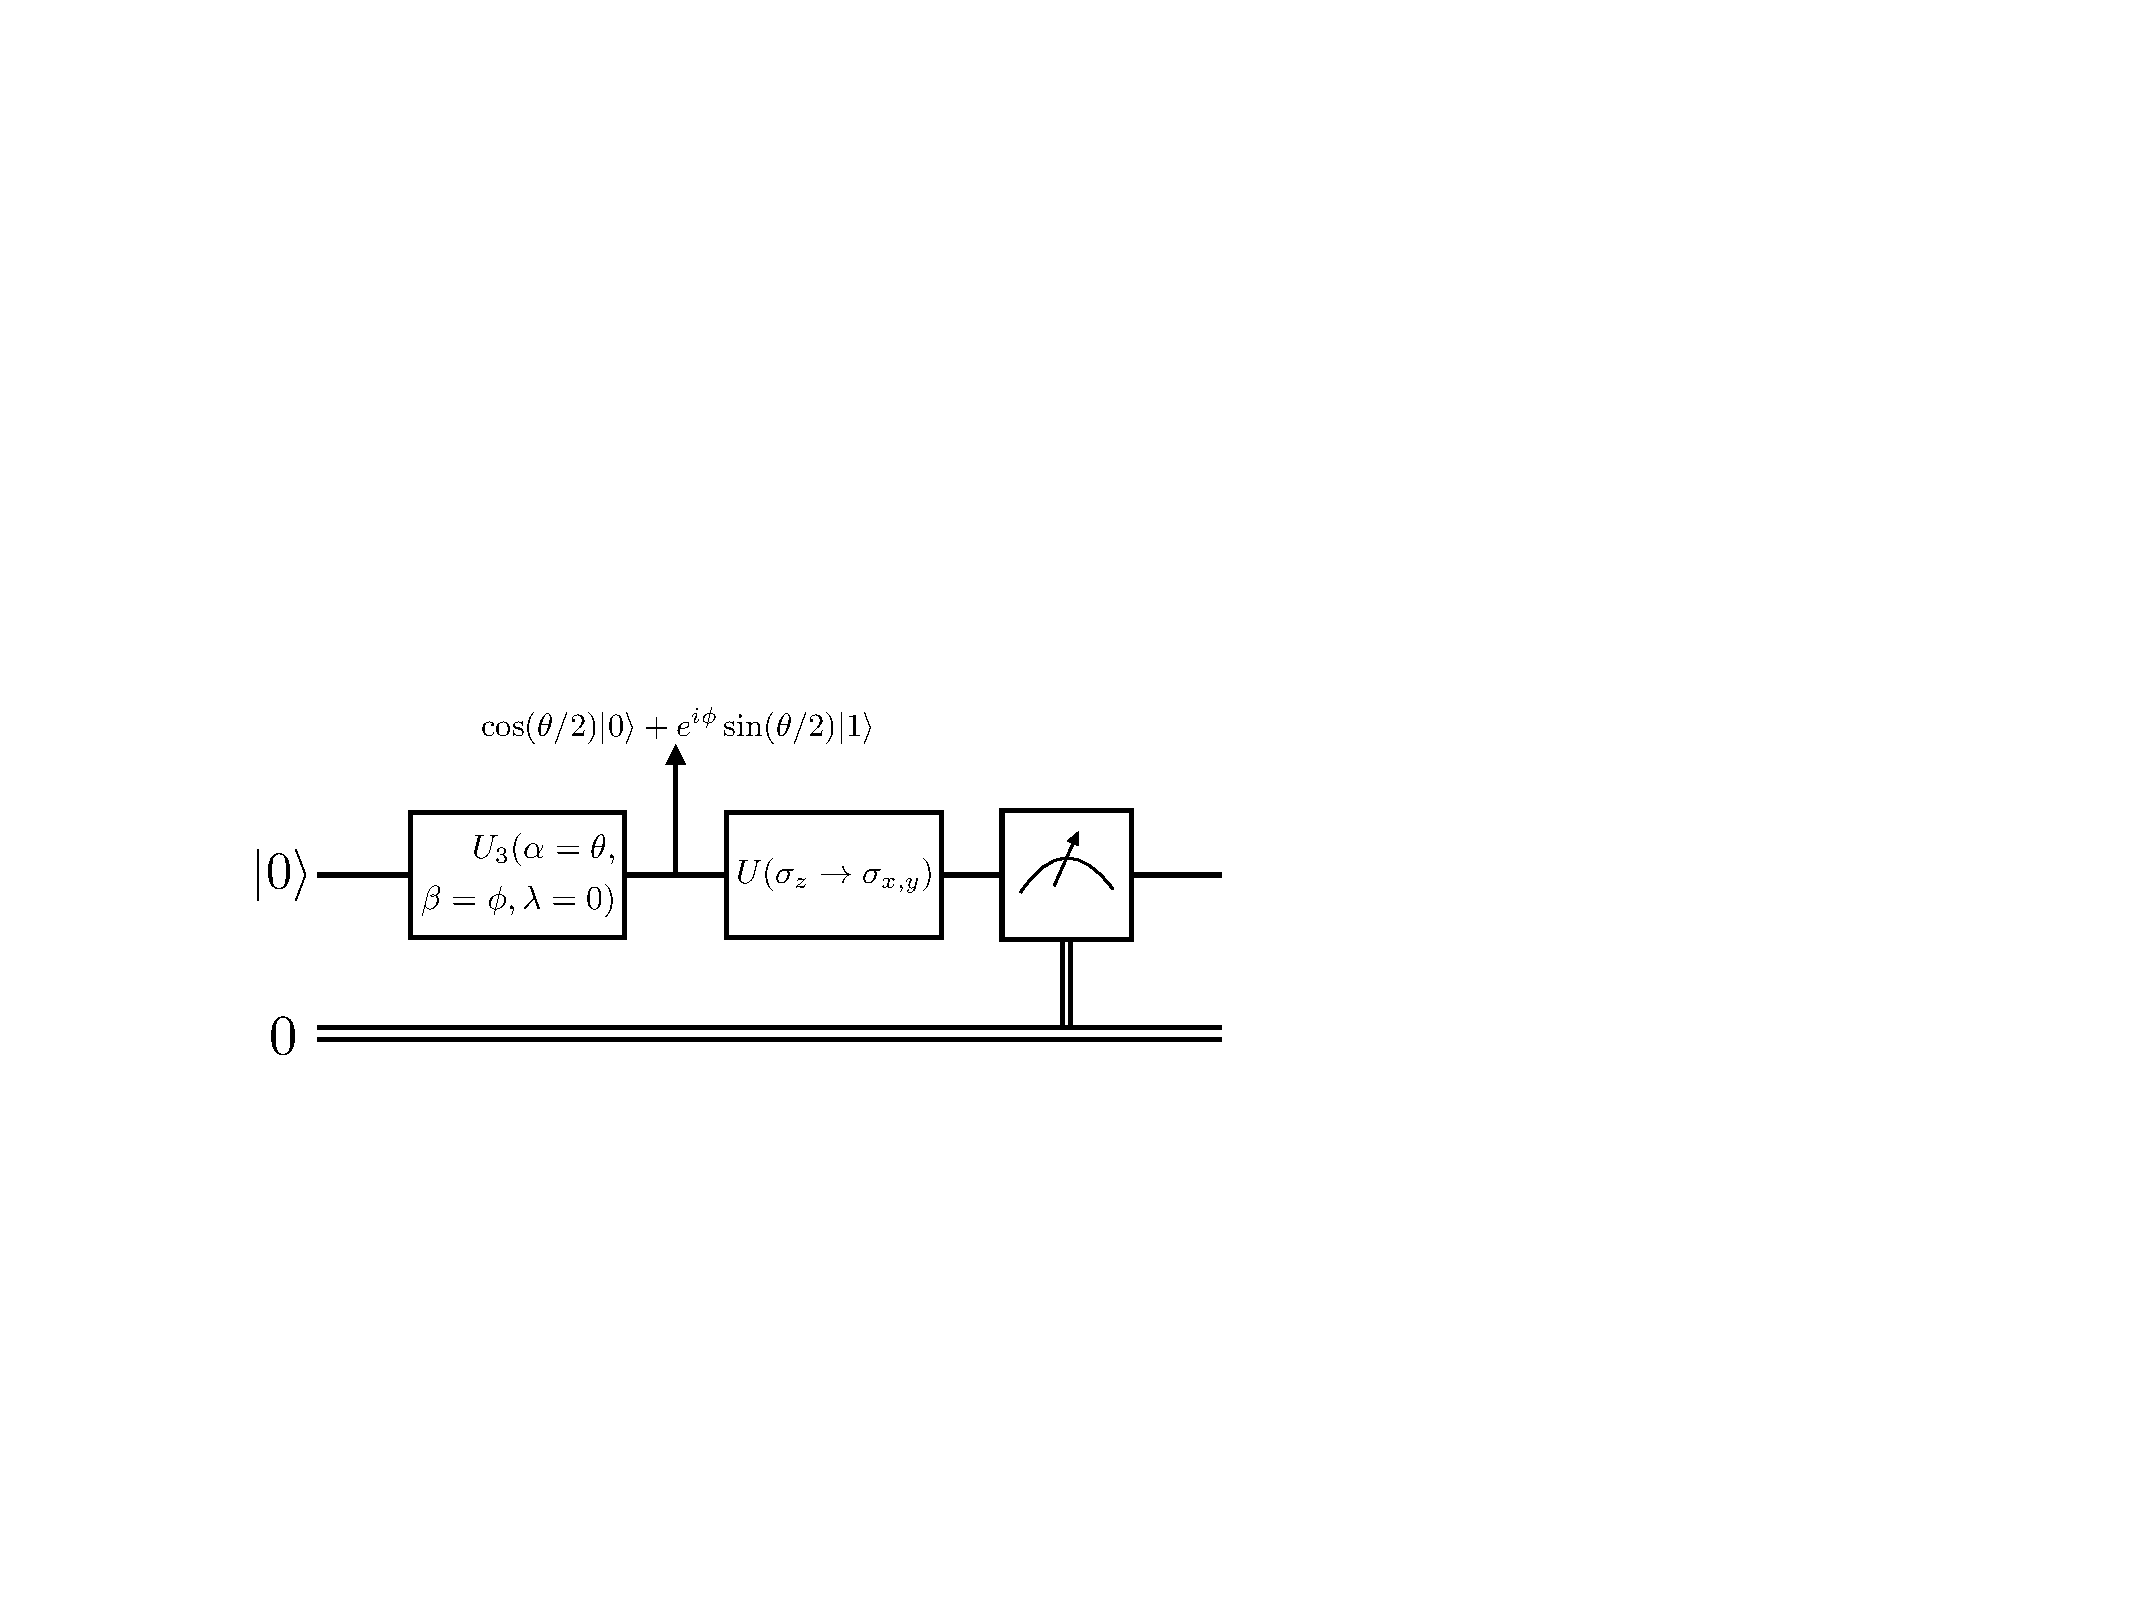
\includegraphics[width=0.5\textwidth]{Scheme.pdf}
       \caption{\label{FIG_01: Scheme} Quantum circuit used.} 
    \end{figure*} 
    
In order to test our circuit, we will run it with the qasm simulator of Qiskit (collecting $2\cdot 10^3$ measurements for the statistics) and then compare the output probabilities with the analytical ones. Consider we start with state $|\psi \rangle = \cos(\theta /2)|0\rangle + e^{i\phi}\sin(\theta /2)|1\rangle$, the probabilities of measuring it in the states of the basis of $\sigma_x$ and $\sigma_y$ are: 

$$
\begin{aligned}
    P\left(|+\rangle_x = \frac{1}{\sqrt{2}}(|0\rangle +|1\rangle)\right) &=& \frac{1}{2}\left(1+\sin(\theta)\cos(\phi) \right);\\
    P\left(|-\rangle_x = \frac{1}{\sqrt{2}}(|0\rangle -|1\rangle)\right) &=& \frac{1}{2}\left(1-\sin(\theta)\cos(\phi) \right);\\
    P\left(|+\rangle_y = \frac{1}{\sqrt{2}}(|0\rangle +i|1\rangle)\right) &=& \frac{1}{2}\left(1-\sin(\theta)\sin(\phi) \right);\\
    P\left(|-\rangle_y = \frac{1}{\sqrt{2}}(|0\rangle -i|1\rangle)\right) &=& \frac{1}{2}\left(1+\sin(\theta)\sin(\phi) \right).\\
\end{aligned}
$$

In order to compare the analytical probabilities versus the simulated ones, with the circuit in Figure~\ref{FIG_01: Scheme} we generated $200$ random initial states (random uniformly distributed values of $\theta\in[0,\pi]$ and $\phi\in[0,2\pi]$) and then measured them either in the $\sigma_x$ or $\sigma_y$ basis. Figure~\ref{FIG_02: Probabilities} shows simulated versus analytical probabilities when measuring the random states in $\sigma_x$ and $\sigma_y$ basis. It shows that, up to small statistical deviations from the simulated probabilities, the circuit and analytical values exactly agree in all cases. This proves that indeed we can measure the states in any basis we want by rotating the state before the measurement.

    \begin{figure*}[h]
        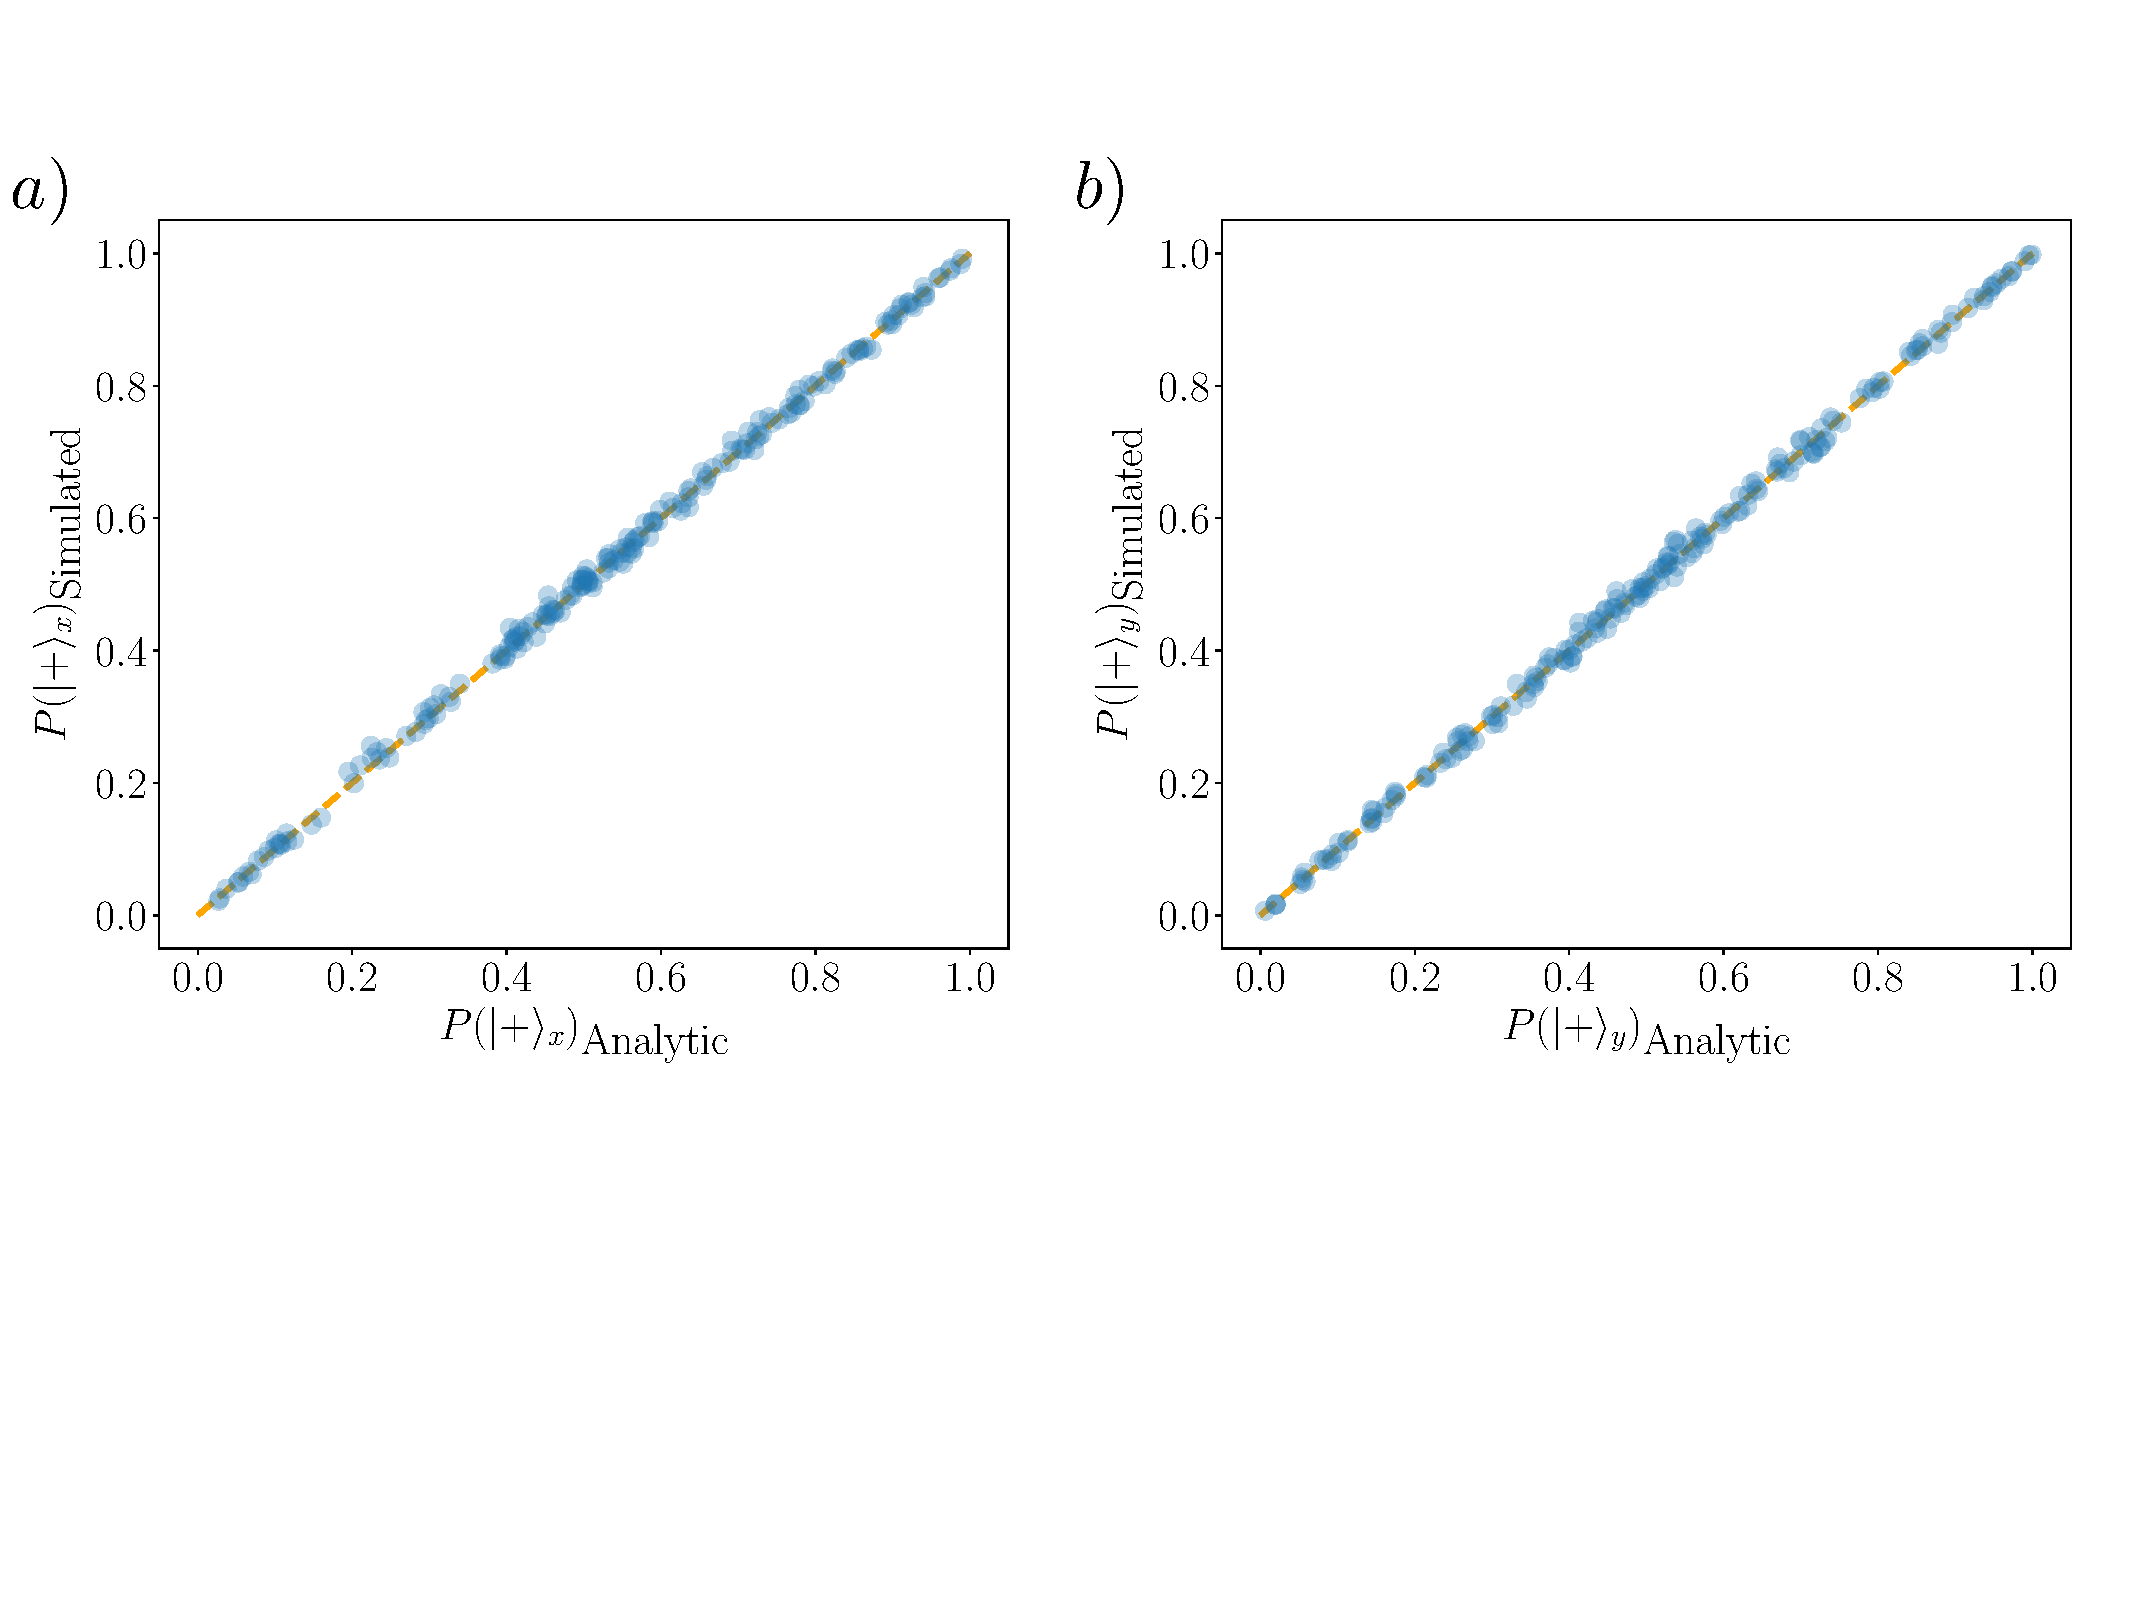
\includegraphics[width=0.8\textwidth]{Probabilities.pdf}
       \caption{\label{FIG_02: Probabilities} Probabilities simulated from circuit in Figure~\ref{FIG_01: Scheme} versus the analytical expected values. Blue dots indicate the probabilities and the dashed orange line is for visual guidance. \textbf{a)} Measuring the initial random states in the $\sigma_x$ basis.\textbf{b)} Measuring the initial random states in the $\sigma_y$ basis.} 
    \end{figure*} 


%%%%%% --------------------- Q2

\subsection*{Q2}
Coherent state is nothing more than a displaced vacuum state:
\begin{equation}
    \ket{\alpha} = U(\alpha)\ket{0}
\end{equation}

Find the transformed operators in terms of original ones (a and a dagger):

\begin{equation}
    \tilde{a} = U^{\dagger}_\alpha a U_\alpha
\end{equation}

\begin{equation}
    {\tilde{a}}^{\dagger} = U^{\dagger}_\alpha a^{\dagger} U_\alpha
\end{equation}
Remember:
\begin{equation}
    a\ket{\alpha} = \alpha\ket{\alpha}
\end{equation}

\subsection*{Solution}



A coherent state $\ket{\alpha}$ may be defined as the unique eigenstate of the annihilation operator $a$ with corresponding eigenvalue $\alpha \in \mathbb{C}$,

\begin{equation}
    a\ket{\alpha} = \alpha\ket{\alpha}.
    \label{eq:eigenvalue-problem}
\end{equation}

The formal solution to this eigenvalue problem is the vacuum state $\ket{0}$ displaced in phase space by $\alpha$:
\begin{equation}
    \ket{\alpha} = D(\alpha)\ket{0},
    \qq{with} D(\alpha) = e^{\alpha a^\dag - \alpha^* a},
    \label{eq:displacement-operator}
\end{equation}
where $D(\alpha)$ is the displacement operator.\footnote{$D(\alpha) \equiv U_\alpha$, the notation given in the problem statement.} It is easy to derive the former relations by writing $|\alpha\rangle = \sum_n \psi_n |n\rangle$ and plugging into the eigenvalue problem:
\begin{equation}
    a\ket{\alpha} = \alpha\ket{\alpha}\ \Longrightarrow\ \sum_n \psi_n a |n\rangle = \sum_n \alpha \psi_n |n\rangle\ \Longrightarrow\  \sum_{n=1}^\infty \psi_n  \sqrt{n} |n-1\rangle = \sum_{n=0}^\infty \alpha \psi_n |n\rangle\
    \label{eq:eigenvalue-problem-derivation}
\end{equation}
which implies the recursion relation
\begin{equation}
    \psi_{n+1}\sqrt{n+1} = \alpha\psi_n \Longrightarrow\ \psi_n = \frac{\alpha^n}{\sqrt{n!}}\psi_0.
\end{equation}
Therefore, the state $\ket{\alpha}$ can be written as:
\begin{equation}
    \ket{\alpha} =\psi_0 \sum_n\frac{\alpha ^n}{\sqrt{n!}}\ket{n} = \psi_0 \sum_n \left( \frac{(\alpha a^{\dagger})^n}{n!} \right) \ket{0} = \psi_0 e^{\alpha a^{\dagger}} \ket{0}.
%    \label{eq:state alpha}
\end{equation}
In principle, we could think of writing $D(\alpha) = e^{\alpha a^{\dagger}}$, however this operator is not unitary and therefore it does not preserve the norms of states. In the previous derivation, the normalization of the wave function is encoded in $\psi_0$, but we can just take $D(\alpha)$ to be unitary and therefore we will not have to worry about $\psi_0$. The easiest way to make that operator unitary is to multiply by the inverse of its complex conjugate, $e^{-\alpha^*a}$. The inverse of the complex conjugate will not change its action over $\ket{0}$ as  $e^{-\alpha^*a}\ket{0} = \ket{0}$. Therefore:
\begin{equation}
    \ket{\alpha} =   e^{\alpha a^{\dagger}-\alpha^*a} \ket{0} \Longrightarrow D(\alpha) = e^{\alpha a^\dag - \alpha^* a}
%    \label{eq:state alpha}
\end{equation}

Finally, we wish to compute $\tilde{a} = D^\dag(\alpha) a D(\alpha)$ and $\tilde{a}^\dag = D^\dag(\alpha) a^\dag D(\alpha)$. Using the expression for the displacement operator \eqref{eq:displacement-operator}, we have
\begin{alignat}{1}
    \tilde{a} &= e^{\alpha^*a - \alpha a^\dag} a e^{\alpha a^\dag - \alpha^* a} \\
    \tilde{a}^\dag &= e^{\alpha^*a - \alpha a^\dag} a^\dag e^{\alpha a^\dag - \alpha^* a}.
    \label{eq:transformed}
\end{alignat}
These are easily computed using the Baker-Hausdorff lemma \cite[Eq. 2.3.47]{sakurai},
\begin{equation}
    e^{iG\lambda}Ae^{-iG\lambda}
    = A + i\lambda\comm{G}{A}
    + \frac{(i\lambda)^2}{2!}\comm{G}{\comm{G}{A}} + \cdots
    + \frac{(i\lambda)^n}{n!} \comm{G}{\comm{G}{\comm{G}{\ldots\comm{G}{A}}}\ldots} + \cdots,
    \label{eq:baker-hausdorff}
\end{equation}
for some operator $A$, where $G$ is Hermitian and $\lambda$ is a real parameter. Identifying $iG = \alpha^*a - \alpha a^\dag$ and $\lambda = 1$, we compute the commutators
\begin{alignat}{3}
    \comm{G}{a} &= -i\comm{\alpha^*a - \alpha a^\dag}{a} &&=& i\alpha\comm{a^\dag}{a} &= -i\alpha \\
    \comm{G}{a^\dag} &= -i\comm{\alpha^*a - \alpha a^\dag}{a^\dag} &&=& -i\alpha^*\comm{a}{a^\dag} &= -i\alpha^*
\end{alignat}
where we have used $\comm{a}{a^\dag} = 1$. As these are each proportional to the identity, all subsequent commutators in \eqref{eq:baker-hausdorff} vanish, so \eqref{eq:transformed} reduces to
\begin{alignat}{1}
    \tilde{a} &= a + \alpha \\
    \tilde{a}^\dag &= a^\dag + \alpha^*.
\end{alignat}



%%%%%% --------------------- Q3

\subsection*{Q3}
Consider a phenomenological Hamiltonian:
\begin{equation}
    H_T = -\frac{E_J}{2} \sum_N
    \left[\ketbra{N+1}{N} + \ketbra{N}{N+1}\right]
\end{equation}
as a representation of the microscopic tunneling of Cooper pairs across the JJ, where state $\ket{N}$ represents the integer N number of excess Cooper pairs in the “box”. Let’s also define a set of phase states $\ket{\delta}$ which are the Fourier dual to the number states  $\ket{N}$, $
    \ket{\delta} = \sum_N e^{iN\delta}\ket{N}$. (Note that the phase $\delta$ lives on the compact space $[0 $  $ 2\pi]$ as the Cooper pair number N on the “island” is a discrete integer). 
    
    (a) Show that the states $\ket{\delta}$ are eigenstates of $\hat{H}$.
    
    (b) Find the associated eigenvalues. 
    
    c) Find the group velocity: \begin{equation}
    v_g \equiv \frac{1}{\hbar} \pdv{\lambda_{T,\delta}}{\delta}.
\end{equation}
\subsection*{Solution}



The tunneling of Cooper pairs into or out of a Cooper pair box via a Josephson junction may be represented by the Hamiltonian
\begin{equation}
    H_T = -\frac{E_J}{2} \sum_N
    \left[\ketbra{N+1}{N} + \ketbra{N}{N+1}\right]
    \label{eq:tunneling-hamiltonian}
\end{equation}
where $E_J$ is the Josephson energy, $\ket{N}$ is the state of the box containing an excess of $N$ Cooper pairs relative to the number of Cooper pairs outside the box,\footnote{For $N<0$, this represents a \emph{deficit} of $N$ Cooper pairs in the box, relative to the number outside the box.} and the sum ranges over all integers $N \in \mathbb{Z}$.
The phase states $\ket{\delta}$ are Fourier dual to the number states $\ket{N}$,
\begin{equation}
    \ket{\delta} = \sum_N e^{iN\delta}\ket{N}.
    \label{eq:phase-states}
\end{equation}

The action of the Hamiltonian \eqref{eq:tunneling-hamiltonian} on the phase states \eqref{eq:phase-states} yields
\begin{alignat}{1}
    H_T\ket{\delta}
    &= -\frac{E_J}{2}
    \sum_N \sum_{N'}
    e^{iN'\delta} \left\{
        \ket{N+1}\braket{N}{N'} + \ket{N}\braket{N+1}{N'}
    \right\} \\
    &= -\frac{E_J}{2}
    \sum_N \sum_{N'}
    e^{iN'\delta} \left\{
        \ket{N+1}\delta_{N,N'} + \ket{N}\delta_{N+1,N'}
    \right\} \\
    &= -\frac{E_J}{2}
    \sum_N
    \left\{
        e^{iN\delta}\ket{N+1} + e^{i(N+1)\delta}\ket{N}
    \right\} \label{eq:before-shift} \\
    &= -\frac{E_J}{2}
    \sum_N
    \left\{
        e^{i(N-1)\delta}\ket{N} + e^{i(N+1)\delta}\ket{N}
    \right\} \label{eq:after-shift} \\
    &= -\frac{E_J}{2}(e^{-i\delta} + e^{+i\delta})
    \sum_N e^{iN\delta} \ket{N} \\
    &= -E_J\cos\delta\ket{\delta}
\end{alignat}
where, in going from \eqref{eq:before-shift} to \eqref{eq:after-shift}, we were able to take $N \rightarrow N-1$ in just the first term because the sum ranges from $-\infty$ to $\infty$. Therefore, the phase states $\ket{\delta}$ are eigenstates of the tunneling Hamiltonian $H_T$ with corresponding eigenvalues $-E_J\cos\delta$, for $\delta \in [0, 2\pi]$.

Assuming $\lambda_{T,\delta} = -E_J\cos\delta$, i.e. the energy of state $\ket{\delta}$ associated with tunneling, the group velocity is
\begin{equation}
    v_g \equiv \frac{1}{\hbar} \pdv{\lambda_{T,\delta}}{\delta} = \frac{E_J}{\hbar}\sin\delta.
\end{equation}
%%%%%% --------------------- Q4

\subsection*{Q4}

Can you always take the square root of a unitary matrix? That is, given a unitary $U$, does there always exist a $\sqrt{U}$ such that $\sqrt{U}\sqrt{U} = U$?

\subsection*{Solution}
Yes, but the square root is not unique. By definition, a complex square matrix $U$ is unitary iff its conjugate transpose is also its inverse:
\begin{equation}
    U\ \text{is unitary}\ \Longleftrightarrow\ U^\dag = U^{-1},
    \label{def:unitary}
\end{equation}
where the inverse of $U$, denoted $U^{-1}$, is defined as the matrix that, when left- or right-multiplied by $U$, produces the identity:
\begin{equation}
    U^{-1}\ \text{is the inverse of}\ U\ \Longleftrightarrow\
    UU^{-1} = U^{-1}U = \id.
    \label{def:inverse}
\end{equation}
It immediately follows that $U$ is normal. By definition, a complex square matrix $N$ is normal iff it commutes with its conjugate transpose:
\begin{equation}
    N\ \text{is normal} \Longleftrightarrow NN^\dag = N^\dag N.
    \label{def:normal}
\end{equation}
Therefore, by definitions \eqref{def:unitary} and \eqref{def:inverse},
\[UU^\dag = \id = U^\dag U \Longrightarrow U\ \text{is normal.}\]

Furthermore, a matrix is normal iff it is unitarily diagonalizable.\footnote{This is a version of the spectral theorem.} Consider the forward direction. By the Schur decomposition, any complex square matrix $U$ can be written
\begin{equation}
    U = VDV^\dag,
    \label{eq:schur}
\end{equation}
where $V$ is unitary and $D$ is upper-triangular. Then $UU^\dag = V(DD^\dag)V^\dag$ by unitarity of $V$, and likewise $U^\dag U = V(D^\dag D)V^\dag$. If $U$ is normal, then $DD^\dag = D^\dag D$ and $D$ is also normal. Hence $D$ is in fact diagonal, since a normal upper-triangular matrix can only have nonzero elements along the diagonal (this follows trivially from the definition \eqref{def:normal} and upper-triangularity). Thus $U$ is unitarily diagonalizable.

%Now, consider the square root of the diagonal matrix $D$, denoted $D^{1/2}$, which by definition satisfies
%\begin{equation}
%    \left(D^{1/2}\right)^2 = D.
%    \label{eq:sqrt-D}
%\end{equation}
%The matrix $D^{1/2}$ is simply a\footnote{In general, there will be 2 square roots for each diagonal element of $D$, but the question asks about existence, not uniqueness.} diagonal matrix whose elements are equal to a square root of the corresponding elements of $D$. We can then construct
%\begin{equation}
%    R = VD^{1/2}V^\dag,
%    \label{eq:sqrt-U}
%\end{equation}
%which has the property we seek, namely
%\begin{align}
%    R^2 &= (VD^{1/2}V^\dag)(VD^{1/2}V^\dag) && \\
%    &= VD^{1/2}D^{1/2}V^\dag &&\text{by unitarity of $V$} \\
%    &= VDV^\dag &&\text{by \eqref{eq:sqrt-D}} \\
%    &= U &&\text{by \eqref{eq:schur}.}
%\end{align}
%We therefore identify $\sqrt{U} \equiv R$ given by \eqref{eq:sqrt-U}, which always exists by construction.

Given that $U$ can be unitarily diagonalized and given the fact that $U^{\dagger}U = 1$, this implies that the eigenvalues of $U$ can be written as:
\begin{equation}
    \lambda_j = e^{i\phi _j},
    \label{eq:EigenvaluesU}
\end{equation}
where $\lambda_j$ designates the $j^{th}$ eigenvalue of $U$. Then,
\[D = \pmqty{\dmat{\ddots,\lambda_j,\ddots}}\]
In the basis where $U$ is diagonal, its square root is obtained simply by taking the square root of the eigenvalues, i.e.
\[D^{1/2} = \pmqty{\dmat{\ddots,\sqrt{\lambda_j}_\pm,\ddots}}.\]
However, for each eigenvalue, there are two possible values of the square root:
\begin{equation}
    \sqrt{\lambda_j}_+ = e^{i\phi _j/2} \; \; \textrm{and} \; \; \sqrt{\lambda_j}_- = e^{i(\phi _j/2+\pi)}.
    \label{eq:RootEigenvalues}
\end{equation}
If matrix $U \in \mathbb{C}^{N\times N}$, then there are $2^N$ possible combinations of  $\sqrt{\lambda_j}_+$ and $\sqrt{\lambda_j}_-$. Therefore, a unitary matrix has a square root, but there are $2^N$ different $\sqrt{U}$. By construction, in the original basis
\[\sqrt{U} = VD^{1/2}V^\dag.\]


%%%%%% --------------------- Q5
\subsection*{Q5}

Prove the following points:
\begin{enumerate}[label=\alph*)]
    \item Two quantum states will lead to different probabilities iff they have different density matrices.
    
    \item No-communication theorem: if Alice and Bob share an entangled state, nothing Alice chooses to do will have any effect on Bob's density matrix $\rightarrow$ There is no observable effect on Bob's end.
\end{enumerate}

\subsection*{Solution}
\begin{enumerate}[label=\alph*)]
\item 


    Suppose we measure a mixed state  $(p_i, \ket{\psi_i}) $ in an orthonormal basis $\ket{\beta_k}$.
    Let's calculate the outcome:
    
    We denote the probability of measuring $\ket{\beta_k}$ by $\Pr[k]$. Then
        \begin{alignat}{1}
            \Pr[k] 
            &= \sum_{j} p_j \mid  {\braket{\psi_j}{\beta_k}} \mid ^2 \\
            &= \sum_{j} p_j {\braket{\beta_k}{\psi_j}}{\braket{\psi_j}{\beta_k}} \\
            &= \bra{\beta_k} \sum_{j} p_j \ketbra{\psi_j}{\psi_j} \ket{\beta_k} \\
            &= \bra{\beta_k} \rho \ket{\beta_k}
        \end{alignat}
        
        Therefore different probabilities (LHS) will lead us different density matrices (RHS) and vice versa.



\item Consider an arbitrary bipartite state,
\[\rho = \sum_{ijk\ell}\rho_{ijk\ell}
\underbrace{\ketbra{i}{j}}_\text{A} \otimes
\underbrace{\ketbra{k}{\ell}}_\text{B},\]
where we take the bases in each subspace to be orthonormal without loss of generality. The reduced density matrix for Bob is\footnote{The trace is basis-independent. For simplicity and without loss of generality, we take the trace with respect to the same orthonormal basis in which Alice's subspace is decomposed.}
\begin{align}
    \rho_B &= \Tr_A\rho && \\
    &= \sum_m \ev{\rho}{m}
        &&\qq{note:} \ket{m} \in \mathcal{H}_A \\
    &= \sum_{ijk\ell m}\rho_{ijk\ell}
        \braket{m}{i}\braket{j}{m} \ketbra{k}{\ell}
        &&\qq{note:} \braket{m}{i} = \delta_{mi},\
            \braket{j}{m} = \delta_{jm} \\
    &= \sum_{k\ell m}\rho_{mmk\ell} \ketbra{k}{\ell}. && \label{eq:bob}
\end{align}
Suppose Alice performs a local unitary operation, $U : \mathcal{H}_A \rightarrow \mathcal{H}_A$, on her subsystem. The new bipartite state becomes
\begin{align}
    \rho' &= U\rho U^\dag\\
    &= \sum_{ijk\ell}\rho_{ijk\ell}
        U\ketbra{i}{j}U^\dag \otimes \ketbra{k}{\ell},
\end{align}
yet Bob's reduced density matrix remains invariant:
\begin{align}
    \rho_B &= \Tr_A\rho' && \\
    &= \sum_{ijk\ell m}\rho_{ijk\ell}
        \mel{m}{U}{i}\mel{j}{U^\dag}{m} \ketbra{k}{\ell}
        &&\qq{commute scalar matrix elements} \\
    &= \sum_{ijk\ell m}\rho_{ijk\ell}
        \mel{j}{U^\dag}{m}\mel{m}{U}{i} \ketbra{k}{\ell}
        &&\qq{remove identity} \sum_m\ketbra{m} = \id \\
    &= \sum_{ijk\ell}\rho_{ijk\ell}
        \mel{j}{U^\dag U}{i} \ketbra{k}{\ell}
        &&\qq{by unitarity,} U^\dag U = \id \\
    &= \sum_{ijk\ell}\rho_{ijk\ell}
        \braket{j}{i} \ketbra{k}{\ell}
        &&\qq{by orthonormality,} \braket{j}{i} = \delta_{ji} \\
    &= \sum_{jk\ell}\rho_{jjk\ell} \ketbra{k}{\ell}. && \label{eq:bob2}
\end{align}
In either case, Bob's reduced density matrix \eqref{eq:bob} or \eqref{eq:bob2} is the same.

In particular, even if $\rho$ is maximally entangled (and therefore pure), there is no operation Alice can perform on her subsystem that will be observable by Bob. Therefore, entanglement does not enable faster-than-light communication.
\end{enumerate}

%%%%%% --------------------- Q6

\subsection*{Q6}
Can different probability distributions over pure states give rise to the same mixed state?

\subsection*{Solution}
Yes. Consider a uniform distribution over the $\sigma_z$ eigenstates,
$\left\{(\frac{1}{2}, \ket{0}), (\frac{1}{2}, \ket{1})\right\}$.
This gives rise to the mixed state
\[\rho = \frac{1}{2}\ketbra{0} + \frac{1}{2}\ketbra{1} = \frac{1}{2}\id\]
in the $\sigma_z$ eigenbasis. However, the identity operator $\id$ has the same representation, $\pmqty{\imat{2}}$, in every orthonormal basis. For instance, consider a uniform distribution over the $\sigma_x$ eigenstates, $\left\{(\frac{1}{2}, \ket{+}), (\frac{1}{2}, \ket{-})\right\}$. This gives rise to the mixed state
\[\rho = \frac{1}{2}\ketbra{+} + \frac{1}{2}\ketbra{-} = \frac{1}{2}\id,\]
now in the $\sigma_x$ eigenbasis. But, noting $\ket{\pm} = \frac{1}{\sqrt{2}}(\ket{0} \pm \ket{1})$,
\begin{align}
    \id =& \ketbra{+} + \ketbra{-} \\
    =& \frac{1}{2}\left( \ketbra{0}{0} + \ketbra{0}{1} + \ketbra{1}{0} + \ketbra{1}{1} \right)\\
    &+ \frac{1}{2}\left( \ketbra{0}{0} - \ketbra{0}{1} - \ketbra{1}{0} + \ketbra{1}{1} \right)\\
    =& \ketbra{0} + \ketbra{1} = \id.
\end{align}
This is obvious if we consider the unitary transformation $U$ connecting the two bases, whereby $U\id U^\dag = UU^\dag = \id$.

Although one might think that a uniform distribution over $\{\ket{0}, \ket{1}\}$ is physically distinct from a uniform distribution over $\{\ket{+}, \ket{-}\}$---corresponding to, say, an ensemble of spins with half aligned along $+\hat{z}$ and the other half along $-\hat{z}$, versus an ensemble with half along $+\hat{x}$ and half along $-\hat{x}$---in fact, there is no measurement which can distinguish between the two.


%%%%%% --------------------- Q7
\subsection*{Q7}
Find a maximally mixed state of a 2-qubit system.

\subsection*{Solution}
Given the computational basis for a two qubit system, $\{ \ket{00}, \ket{01}, \ket{10}, \ket{11} \}$, the maximally mixed state is an ensemble mix of all the states with equal probability:
\begin{equation}
    \rho = \frac{1}{4}(\ketbra{00}{00}+ \ketbra{01}{01}+ \ketbra{10}{10}+ \ketbra{11}{11} )
\end{equation}
It is trivial to see that the rank of the density matrix is 4, as for a maximally entangled state. In general, for a system of $n$ qubits, with computational basis elements $\{ \ket{i} : i = 0, 1, ..., 2^n-1\}$, the maximally mixed state is: $\rho = \id/2^n$, which has rank $2^n$. The von Neumann entropy of these states is maximal and follows a volume law:
\begin{equation}
    S = -\Tr(\rho \log_2 \rho) = -\sum_{i=0}^{2^n-1}\frac{1}{2^n}\log_2 \frac{1}{2^n} = n.
\end{equation}

%%%%%% --------------------- Q8

\subsection*{Q8}
Implement superdense coding in Qiskit. Attach the code and results.

\subsection*{Solution}

In this case Alice has two classical bits she wants to send to Bob by just sending one quantum bit. In the following implementation we will map all $4$ possible combinations of the two bits to integers from $0$ to $3$: $00\rightarrow 0$, $01\rightarrow 1$, $10\rightarrow 2$ and $11\rightarrow 3$.

The algorithm proceeds as follows:
\begin{enumerate}
    \item Alice decides which combination of two classical bits she wants to send between possibilities $0$ to $3$. In the qiskit implementation this is stored in variable "bit". In this example Alice wants to send $11$ to Bob:
    \begin{lstlisting}[language=Python]
    #Usual imports
    import qiskit
    import numpy as np
    
    bit = 3
    \end{lstlisting}

    \item Alice and Bob share a maximally entangled qubit pair: $\ket{\psi_0} = \frac{1}{\sqrt{2}}(\ket{0_A0_B} + \ket{1_A1_B})$. In this notation the most significant bit corresponds to Alice. The initial state of the qubits is $\ket{00}$. Therefore, to put the system into state $\ket{\psi_0}$ we apply a Hadamard gate on Alice's qubit and a CNOT(A$\rightarrow$B) gate where the control qubit is Alice's and the target one is Bob's ($\ket{\psi_0} = \textrm{CNOT(A} \rightarrow \textrm{B)} H(A)\ket{00}$):
    \begin{lstlisting}[language=Python]
    #Define the quantum circuit with two classical 
    #registers and two qubits
    qc = QuantumCircuit(2,2)
    
    #Create the entangled pair shared by Alice and Bob
    qc.h(0) #Hadamard on 0
    qc.cx(0,1) #CNOT where 0 is the control and 1 is target
    \end{lstlisting}
    \item Alice performs one operation on her qubit depending on what pair of classical bits she wants to send:
    \begin{align}
   & 00 \rightarrow \id_A \otimes \id_B \ket{\psi_0} = \ket{\psi_{00}} \frac{1}{\sqrt{2}}(\ket{0_A0_B} + \ket{1_A1_B}) \\
    & 01 \rightarrow X_A \otimes \id_B \ket{\psi_0} = \ket{\psi_{01}} \frac{1}{\sqrt{2}}(\ket{0_A1_B} + \ket{1_A0_B})\\
    & 10 \rightarrow Z_A \otimes \id_B \ket{\psi_0} = \ket{\psi_{10}} \frac{1}{\sqrt{2}}(\ket{0_A0_B} - \ket{1_A1_B})\\
    & 11 \rightarrow ZX_A \otimes \id_B \ket{\psi_0} = \ket{\psi_{11}} \frac{1}{\sqrt{2}}(\ket{0_A1_B} - \ket{1_A0_B}).
    \end{align}
    Which in Qiskit is implemented as follows:
    \begin{lstlisting}[language=Python]
    if bit == 1: #Sending 01
        qc.x(0)
    if bit == 2: #Sending 10
        qc.z(0)
    if bit == 3: #Sending 11
        qc.x(0)
        qc.z(0)
    \end{lstlisting}
    \item Alice sends her qubit to Bob over a quantum channel. Nothing to do on Qiskit.
    \item Bob, who now has the two qubits, applies a CNOT(A$\rightarrow$B) gate and then applies a Hadamard gate to the qubit that used to belong to Alice. Bob obtains the following set of orthogonal states depending on what qubit Alice sent him:
    \begin{align}
   & 00 \rightarrow  H_A \otimes \id_B  \cdot \textrm{CNOT(A} \rightarrow \textrm{B)} \ket{\psi_{00}} =  \ket{00}\\
    & 01 \rightarrow H_A \otimes \id_B  \cdot \textrm{CNOT(A} \rightarrow \textrm{B)} \ket{\psi_{01}} =  \ket{01}\\
    & 10 \rightarrow H_A \otimes \id_B  \cdot \textrm{CNOT(A} \rightarrow \textrm{B)} \ket{\psi_{10}} =  \ket{10}\\
    & 11 \rightarrow H_A \otimes \id_B  \cdot \textrm{CNOT(A} \rightarrow \textrm{B)} \ket{\psi_{11}} =  \ket{11}.\\
    \end{align}
    Bob finally measures the two qubits in the computational basis, obtaining precisely the two classical bits Alice wanted to send. This final step with the simulation of the whole process is implemented in Qiskit:
    \begin{lstlisting}[language=Python]
    qc.cx(0,1) #Applying the CNOT 
    qc.h(0) #Applying the Hadamard to Alice's qubit
    qc.measure(0,0) #Measuring qubit that used to belong to Alice
    qc.measure(1,1) #Measuring qubit that always belonged to Bob
    
    #Simulation using qasm simulator
    Measurements = 2000 #Number of measurements
    emulator = Aer.get_backend('qasm_simulator')
    job = execute( qc, emulator, shots = Measurements )
    hist = job.result().get_counts() #results of the measurement
    print(hist) #Print results
    \end{lstlisting}
\end{enumerate}
The code will be attached in the email as a ``jupyter notebook''. For the results, even using the ``qasm'' simulator, feeding the program with $\textrm{``bit''} = 0$ gave output $00$ with probability exactly $1$. Feeding the program with $\textrm{``bit''} = 1$ gave output $10$ with probability exactly $1$. Feeding the program with $\textrm{``bit''} = 2$ gave output $01$ with probability exactly $1$, and feeding the program with $\textrm{``bit''} = 3$ gave output $11$ with probability exactly $1$. Note that the output for $\textrm{``bit''} = 1$ and $\textrm{``bit''} = 2$ are swapped. This is because Qiskit takes the zeroth qubit to be the least significant one. However, the results are correct.



%%%%%% --------------------- Q9

\subsection*{Q9}
What choice of $\lambda_1, \ldots, \lambda_n$ maximizes the entropy,
\[S(\rho) = -\sum_k\lambda_k\log_2\lambda_k,\]
where $\sum_k\lambda_k = 1$.

\subsection*{Solution}

The von Neumann entropy expressed in units of bits,
\begin{equation}
    S(\rho) = -\sum_k \lambda_k \log_2 \lambda_k,
    \label{eq:von-neumann-entropy}
\end{equation}
may be straightforwardly extremized over all diagonal density operators $\rho$ with eigenvalues $\lambda_k$, subject to the probability conservation constraint,
\begin{equation}
    \sum_k \lambda_k = 1,
    \label{eq:probability-constraint}
\end{equation}
by the method of Lagrange multipliers. We form the Lagrange function
\[\mathcal{L}(\{\lambda_k\}, \eta)
= S(\rho) - \eta\left(\sum_k \lambda_k - 1\right),\]
and then vary each parameter $\{\lambda_k\}, \eta$ independently to find the stationary point in the parameter space. Variation with respect to $\eta$ recovers the probability constraint \eqref{eq:probability-constraint}, while variation with respect to each $\lambda_j \in \{\lambda_k\}$ yields
\[\pdv{\mathcal{L}}{\lambda_j} = -(\log_2\lambda_j + 1) - \eta = 0, \quad \forall\ j\]
which must vanish at the stationary point. This implies
\[\lambda_j = 2^{-(\eta + 1)}, \quad \forall j,\]
i.e. all $\lambda_j$'s are equal to the same constant. Enforcing the probability constraint \eqref{eq:probability-constraint} determines $\eta$ such that
\[\lambda_j = 2^{-n} = \frac{1}{D}, \quad \forall j\]
for $n$ qubits, or Hilbert space dimension $D = 2^n$. Therefore, the von Neumann entropy is maximized\footnote{One can verify this extremum is a maximum using a \href{https://en.wikipedia.org/wiki/Hessian_matrix\#Bordered_Hessian}{bordered Hessian} test.} when $\{\lambda_k\}$ is a uniform distribution, i.e. when $\rho$ is a ($\sim$ classical) maximally mixed state. Moreover, this state is unique.

In the above, we assumed $\rho$ is diagonal, but note that any $\rho$ can be diagonalized and the von Neumann entropy is basis-independent, as
\begin{align}
\rho &= U\rho_d U^{\dagger} \\
\implies S &= -\Tr(\rho \ln\rho) \\
&= -\Tr(U\rho_d U^{\dagger} \ln[U\rho_d U^{\dagger}]) \\
&= -\Tr(U \rho_d U^{\dagger} [U\ln(\rho_d)U^{\dagger}]) \\
&= -\Tr(U\rho_d  \ln(\rho_d)U^{\dagger}) \\
&= -\Tr(\rho_d \ln\rho_d)
\end{align}
where the final equality follows the cyclicity of the trace.

For the sake of completeness, note that since $0 \leq \lambda_k \leq 1\ \forall k$, the von Neumann entropy $S(\rho) \geq 0$ according to \eqref{eq:von-neumann-entropy}. This lower bound is attained for $\lambda_k = 1$ for some particular $k$ and $\lambda_k = 0$ for all others. This occurs for any $\rho$ representing a pure state. So we conclude
\begin{equation}
    0 \leq S(\rho) \leq \ln D
\end{equation}
where the upper bound is attained for the (unique) maximally mixed state $\rho = \id/D$, while the lower bound is attained for every (i.e. not unique) pure state $\rho$.

%%%%%% --------------------- Q10

\subsection*{Q10}
1D harmonic oscillator:
\[H\ket{n} = \hbar\omega(n+\frac{1}{2})\ket{n}\]
\[a\ket{\alpha} = \alpha\ket\alpha\]
\[\ket\alpha, (\abs{\alpha}, n)\]
\begin{enumerate}[label=\alph*)]
    \item Time evolution of coherent state.
    \item Calculate:
        \[\ev{x(t)} = \ev{x}{\alpha(t)}\]
        \[\ev{p(t)} = \ev{p}{\alpha(t)}\]
    \item Consider the mixed state:
        \[\rho = \frac{1}{2\pi} \int_0^{2\pi}\dd{\phi} \ketbra{\abs{\alpha} \exp(i\phi)},\]
        a mixture of coherent states with random phase and fixed amplitude $\abs{\alpha}$. Show this is equivalent to a mixture of coherent states with a Poisson distribution with $\bar{n} = \abs{\alpha}^2$.
\end{enumerate}

\subsection*{Solution}

\begin{enumerate}[label=\alph*)]
\item %Let us start by inserting the completeness relation of the occupation number states
%\begin{equation}
%    \ket{\alpha} = \sum_n \ket{n} \braket{n}{\alpha}
%\end{equation}
%Then we calculate the transition amplitude $\braket{n}{\alpha}$, where we multiply the whole eigenvalue equation with $\bra{n}$ from the left:
%\begin{equation}
%    \bra{n} a \ket{\alpha} = \bra{n} \alpha \ket{\alpha}
%    \label{eq:coherent_n}
%\end{equation}
%Using the properties of $a$ and $a^{\dagger}$ operators, we rewrite the left side of Eq.\ref{eq:coherent_n}.
%\begin{equation}
%     a^{\dagger} \ket{n} = \sqrt{n+1} \ket{n+1} \rightarrow \bra{n} a =\sqrt{n+1} \bra{n+1}
%\end{equation}
%\begin{equation}
%    \sqrt{n+1} \braket{n+1}{\alpha} = \alpha \braket{n}{\alpha}
%\end{equation}
%And replace the occupation number n with n-1 to obtain
%\begin{equation}
%    \braket{n}{\alpha}  = \frac{\alpha}{ \sqrt{n} } \braket{n-1}{\alpha}
%    \label{eq:expanding_n}
%\end{equation}
%By iterating the last step, i.e. again replacing n with n-1 in Eq.\ref{eq:expanding_n} and reinserting the result on the right hand side, we get
%\begin{equation}
%    \braket{n}{\alpha} = \frac{\alpha^2}{\sqrt{n(n-1)}} \braket{n-2}{\alpha} = ... = \frac{\alpha^n}{\sqrt{n!}} \braket{0}{\alpha} 
%\end{equation}
%Which results in 
%\ke

We first expand the coherent state $\ket{\alpha}$ in the Fock basis (derived in our solution to HW2 Problem 2), as
\begin{equation}
    \ket{\alpha} = e^{-\frac{1}{2}|\alpha|^2} \sum_{n=0}^{\infty} \frac{\alpha^n}{\sqrt{n!}} \ket{n}.
    \label{eq:coherent-state}
\end{equation}

The time evolution of the coherent state is then obtained by time-evolving the individual Fock-state components. These are energy eigenstates of the harmonic oscillator with energy $E_n = \hbar\omega (n+\frac{1}{2})$. Their time evolution follows from the Schr\"odinger equation as
\begin{equation}
    \ket{n} \longrightarrow e^{-in\omega t} e^{-\frac{i\omega t}{2}}\ket{n},
\end{equation}
which yields the time-evolved coherent state
\begin{equation}
    \ket{\alpha(t)} =
    e^{-\frac{i\omega t}{2} }
    e^{-\frac{1}{2}|\alpha|^2}
    \sum_{n=0}^{\infty}
    \frac{(\alpha e^{-i\omega t})^n}{\sqrt{n!}} \ket{n}
    \label{eq:coherent-state-time-dependent}
\end{equation}

If we define
\begin{equation}
    \alpha(t) = \alpha e^{-i\omega t},
    \label{eq:coherent-state-eigenvalue}
\end{equation}
then $\ket{\alpha(t)}$ is given by Eq.~\eqref{eq:coherent-state} with $\alpha \rightarrow \alpha(t)$, times a global phase factor $\exp(-i\omega t/2)$.

\item We can write the position and momentum operator in terms of creation and annihilation operators:
\[x = \sqrt{\frac{\hbar}{2 m \omega}} (a^\dag + a),
\qquad p = i\sqrt{\frac{m\hbar \omega}{2}} (a^\dag - a).\]
Note that the eigenvalue equation for the coherent state holds at all times,
\[a\ket{\alpha(t)} = \alpha(t)\ket{\alpha(t)},\]
where the eigenvalue is given by Eq.~\eqref{eq:coherent-state-eigenvalue}. It is then straightforward to compute
\begin{alignat}{2}
    \ev{x}{\alpha(t)}
    &= \sqrt{\frac{\hbar}{2 m \omega}}
    (\alpha^* e^{i\omega t} + \alpha e^{-i\omega t})
    &&= x_0 \cos(\omega t - \phi) \\
    \ev{p}{\alpha(t)}
    &= i\sqrt{\frac{m\hbar \omega}{2}}
    (\alpha^* e^{i\omega t} - \alpha e^{-i\omega t})
    &&= -m \omega x_0 \sin(\omega t - \phi),
\end{alignat}
where we have defined $\alpha = \abs{\alpha}e^{i\phi}$ and $x_0 = \abs{\alpha}\sqrt{2\hbar/m\omega}$.


\item In this case we wish to compute the density matrix for the time evolution of state $\ket{\alpha(t)}$ given by Eq.~\eqref{eq:coherent-state-time-dependent}.
By definition, we wish to compute:
\begin{equation}
    \rho  = \frac{1}{2\pi}\int_0^{2\pi}d\phi\ketbra{|\alpha|e^{i\phi}}{|\alpha|e^{i\phi}} = \frac{e^{-|\alpha|^2}}{2\pi}\int_0^{2\pi}d\phi \sum_{m,n}\frac{\left( |\alpha|e^{-i\phi} e^{i \omega t}\right)^n \left( |\alpha|e^{i\phi} e^{-i \omega t}\right)^m}{\sqrt{n!m!}}\ketbra{m}{n}=
\end{equation}
\begin{equation}
     = \sum_{n,m}\frac{e^{-|\alpha|^2} |\alpha|^{n+m}e^{-i \omega t(m-n)} \frac{1}{2\pi}\int_0^{2\pi}d\phi e^{i\phi(m-n)}}{\sqrt{n!m!}}\ketbra{m}{n}
\end{equation}
Now, taking into account that $\frac{1}{2\pi}\int_0^{2\pi}e^{i\phi(m-n)} = \delta_{m,n}$, we end up obtaining:
\begin{equation}
     \rho = \sum_{n = 0}^\infty \frac{e^{-|\alpha|^2} \left(|\alpha|^2\right)^n}{n!}\ketbra{n}{n}
\end{equation}
Finally recalling that Poisson distribution of average $\lambda$ is $f(\lambda, n) = \frac{e^{-\lambda}\lambda^n}{n!}$, we see that our density matrix is poisson distributed with average $|\alpha|^2$.


\end{enumerate}


%%%%%% --------------------- Q11

\subsection*{Q11}
\begin{enumerate}[label=\alph*)]
    \item Design your own quantum bank that produces quantum money.
    \item what are the odds for hacking your quantum money?
\end{enumerate}

\subsection*{Solution}



\begin{enumerate}[label=\alph*)]
    \item In this scheme, a piece of quantum money comprises an $n$-qubit ``bill'' state and a classical serial number. The quantum bank issues money by generating a bill state and assigning it a unique serial number. The description of each issued bill state and its corresponding serial number are stored in a secret ledger maintained by the bank. A vendor, upon receiving a piece of quantum money from a customer, sends the bill state and its serial number to the bank for verification. The bank uses the serial number to look up the bill state description in the ledger and compare it to the bill state received from the vendor. If they match, the transaction is approved.
    
    \item The security and performance of this scheme hinges on how the bank produces the $n$-qubit bill state. One potential method of state generation follows. For each qubit, the bank randomly selects a basis, say $\sigma_x$ or $\sigma_z$, and randomly assigns an eigenstate of that basis to the value of the qubit, i.e. $\ket{0}$ or $\ket{1}$ for $\sigma_z$ and $\ket{+}$ or $\ket{-}$ for $\sigma_x$. The $n$-qubit bill state can then be prepared by single-qubit rotations, with a typical bill state looking something like,
    \[\underbrace{
        \ket{+\ 0\ 1 - + + - 0 + - 1 - 0\ 0\ 1\ 0 + +\ 0\ 0\cdots}.
    }_\text{$n$ qubits}\]
    
    Note that the space complexity for storing the bill description in the ledger is $\mathcal{O}(n)$, since for each qubit we need to store 1 bit specifying the basis and 1 bit specifying the eigenstate. Furthermore, forging bill states is prohibited by the no-cloning theorem, since the counterfeiter does not know the basis used for each qubit. Therefore, possession of a bill state does not allow duplicates to be produced.
    
    Given the serial number, the only counterfeiting strategy is to attempt to guess the bill state. Assuming the counterfeiter knows the basis set $\{\sigma_x, \sigma_z\}$, the probability of guessing the correct basis is 1/2, and the probability of guessing the correct eigenstate within that basis is also 1/2, so the probability of getting the state of any qubit exactly correct is 1/4. However, if the counterfeiter guesses the incorrect basis, it is still possible that the bank measures the correct eigenstate during the verification process. Since each wrong-basis eigenstate is a uniform superposition of the right-basis eigenstates, this occurs with probability 1/2. The probability for the bank to erroneously approve a counterfeit 1-qubit bill state is then
    \begin{align}
        \underbrace{\Pr(\text{right eigenstate}|\text{right basis})}_{1}
        \underbrace{\Pr(\text{right basis})}_{1/2} +
        \underbrace{\Pr(\text{right eigenstate}|\text{wrong basis})}_{1/2}
        \underbrace{\Pr(\text{wrong basis})}_{1/2}
        = 3/4
    \end{align}
    
    For an $n$-qubit bill state, every qubit must be approved individually, with a single wrong outcome identifying a counterfeit. The total probability for the bank to erroneously approve a counterfeit $n$-qubit bill state is then $(3/4)^n$ and is shown in Fig.~\ref{fig:quantum-money}. This scheme is therefore exponentially secure in the number of qubits used for the bill state.\footnote{Note that this security analysis is identical to that of the BB84 protocol. Our quantum money scheme is essentially the same as BB84, with the counterfeiter playing the role of the eavesdropper.}
    \begin{figure}[htpb]
        \centering
        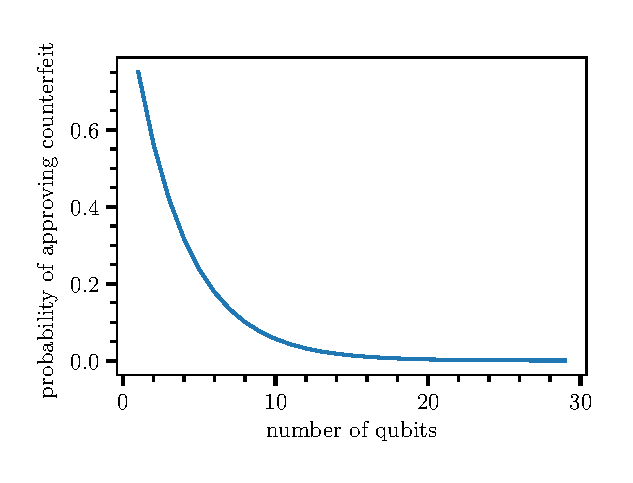
\includegraphics[width=0.6\linewidth]{quantum-money.eps}
        \caption{The probability of approving a counterfeit is $(3/4)^n$ where $n$ is the number of qubits.}
        \label{fig:quantum-money}
    \end{figure}
\end{enumerate}


%%%%%% --------------------- Q12

\subsection*{Q12}
There exist bipartite states that take a lot of entanglement to make but you can only extract a small fraction of the entanglement. Find an example and show $E_f \gg E_D$ can be achieved by extension for larger qubit systems.
\subsection*{Solution}



This question is a very active field of research in the moment and it is actually very complicated to answer. Here we will give a simple toy model answer and describe some of the recent works about this matter.

 One simple case of such bipartite states that take more entanglement to make than the entanglement you can measure is for example a system with 3 qubits. Suppose that subsystem A is qubit 0 and subsystem B is qubits 1 and 2. Now, imagine that qubits 1 and 2 are in a Bell state:
 \begin{equation}
     \ket{\psi}_{1,2} = \frac{\ket{11}_{1,2}+\ket{00}_{1,2}}{\sqrt{2}}
 \end{equation}
 and qubit number 0 is for example in state $\ket{\psi}_{0} = \ket{0}_0$. Then state of the whole system is:
  \begin{equation}
     \ket{\psi}_{0,1,2} = \ket{0}_{0} \otimes \frac{\ket{11}_{1,2}+\ket{00}_{1,2}}{\sqrt{2}}.
 \end{equation}
 In this case, the entanglement of formation is $1$ as we created a Bell pair in qubits 1 and 2, however, the entanglement between subsystem A and subsystem B is zero and therefore we cannot extract any entanglement out of this partition of the state. Therefore $E_D<E_f$.
 
 In the case of having many qubits, we can choose to split the system in a certain way obtaining subsystems A and B. Now imagine that qubits are laid out in a 1D chain and we form a Bell state of nearest neighbours in subsystem A and do the same in subsystem B, but we don't form a Bell pair between the qubits in the boundaries of A and B. In this case, the total number of Bell pairs we needed to form the state was of the order of the number of qubits, but subsystem A is not entangled with subsystem B and therefore the amount of entanglement I get out of this partition is zero and therefore $E_f>>E_D$.

Recent studies focus on the entanglement of formation and distillation from a more systematic point of view. Given $N$ copies of a bipartite state $\rho_{AB}$, we can imagine extracting $M$ copies of a Bell state $\ketbra{\psi^-}$ using only local operations and classical communication (LOCC),
\[\rho_{AB}^{\otimes N} \xrightarrow{\text{LOCC}} \ketbra{\psi^-}^{\otimes M}.\]
This process is known as entanglement concentration or distillation. The \emph{distillable entanglement} $E_D(\rho_{AB})$ is the largest value of $M/N$ attainable as $N \rightarrow \infty$. This can be understood as the largest number of Bell states that can be distilled from the given bipartite state.

Conversely, we can imagine starting with $M$ copies of a Bell state and mixing them into $N$ copies of a given bipartite state using LOCC,
\[\ketbra{\psi^-}^{\otimes M} \xrightarrow{\text{LOCC}} \rho_{AB}^{\otimes N}.\]
This process is known as entanglement dilution. The \emph{entanglement cost} $E_C(\rho_{AB})$ is the \emph{smallest} value of $M/N$ attainable as $N \rightarrow \infty$. It is therefore the asymptotic limit of the entanglement of formation. This can be understood as the smallest number of Bell states required to form the bipartite state.

Since any measure of entanglement cannot increase under LOCC, we must have $E_C(\rho_{AB}) \geq E_D(\rho_{AB})$. Intuitively, one might expect that entanglement distillation and dilution are asymptotically reversible, i.e.
\[\ketbra{\psi^-}^{\otimes M} \xleftrightarrow{\text{LOCC}} \rho_{AB}^{\otimes N},\]
such that the bound is saturated as $N \rightarrow \infty$. Indeed, for pure states, this is in fact the case, and $E_C = E_D = S(\rho_A)$, the von Neumann entropy of the reduced state of $\rho_{AB}$.

For mixed states or multipartite entangled states, however, entanglement distillation/dilution is irreversible in the asymptotic limit, and consequently $E_C > E_D$. These processes can therefore be thought of as a type of lossy compression/decompression algorithm. \citeauthor{horodecki} showed the existence of so-called bound entangled states which require entanglement to create, but from which no entanglement can be distilled. \citeauthor{vidal} generalized this result to the asymptotic limit. Subsequently, \citeauthor{volbrecht} showed that mixtures of maximally entangled states can be diluted and distilled reversibly if and only if they realize the lower bound of the Heisenberg uncertainty principle, demonstrating that irreversibility is a generic and common phenomenon. This remains an active area of research. For a more detailed overview of the various entanglement measures and their associated theorems, see Ref.~\cite{entanglement-review}.


%%%%%% --------------------- Q13

\subsection*{Q13}
Qiskit: Make a circuit to generate a random number between 0 and $2^{3}$-1. What is the entropy? repeat for 0 and $2^{15}$-1. how much does the entropy change?

\subsection*{Solution}

In this case, we will design the simplest random number generator possible, even though in the literature one can find more refined algorithms that take into account that the quantum hardware can be biased (for cryptography applications). These algorithms are all based on the CHSH game with certain variations.

Here we will consider that our quantum hardware is not biased (the NSA has not included a back door) and that therefore we have a perfect quantum device that we have fabricated ourselves. In this case, the task is fairly simple, if we want a random 1-bit generator, we just need to put one qubit in state $\ket{+}$ and measure in the computational basis outputs $\ket{0}$ or $\ket{1}$ with complete randomness and probability $1/2$. Therefore, the protocol is clear if we want to generate a random number between $0$ and $2^n-1$: take $n$ qubits in the computational basis, put all of them in state $\ket{+}$ and measure them in the computational basis. Then, the result of your measurement represents the desired number in binary representation. Note that the random numbers between $0$ and $2^n-1$ will be uniformly sampled with probability $1/2^n$. In this sense, the quantum entropy is $0$ as the state of the system is separable, but the classical entropy of the random number probability distribution is maximal: $S = -\sum_xp_x \log_2 p_x = n$, as $p_x = 1/2^n$ for every random number $x$ generated.

This algorithm can also be done with one qubit, where you prepare it to be in the state $\ket{+}$ and then measure it in the computational basis. The process is repeated $n$ times and the output of the measurements is ordered to generate the desired random number in binary representation as depicted in Figure~\ref{FIG_01: Plot1} a). This approach might be better in terms of accuracy in NISQ devices where we can have one qubit with better fidelity and decay times than the rest and therefore the errors will be smaller by just using this 1-qubit device. This is the reason why we will implement this approach in Qiskit, jut using a circuit with 1 qubit. It also has the advantage that it can be simulated in a classical computer fairly fast. Otherwise it would be pretty hard to simulate the case with $15$ qubits.

The Qiskit code we wrote is fairly simple, it is a fucntion that takes as an input the number of random bits to be generated $n$ and outputs the random distribution as a numpy array. In this case, the quantum circuit described above is simulated using the 'qasm' simulator:

\begin{lstlisting}[language=Python]
##### generate random numbers between 0 and 2^n-1#####
#need to pass n to the function
def RandomNumberGen(n):
    num = np.zeros(n)
    for i in range(n):
        qc = QuantumCircuit(1,1)
        qc.h(0) #get + state
        qc.measure(0,0) #measure in computational basis
        
        #Simulate and get results
        emulator = Aer.get_backend('qasm_simulator')
        job = execute( qc, emulator, shots = 1 )
        hist = job.result().get_counts()
        if hist.get('0') == None:
            num[i] = 1
        if hist.get('1') == None:
            num[i] = 0
    return num
    \end{lstlisting}
    
\begin{figure*}[htpb]
        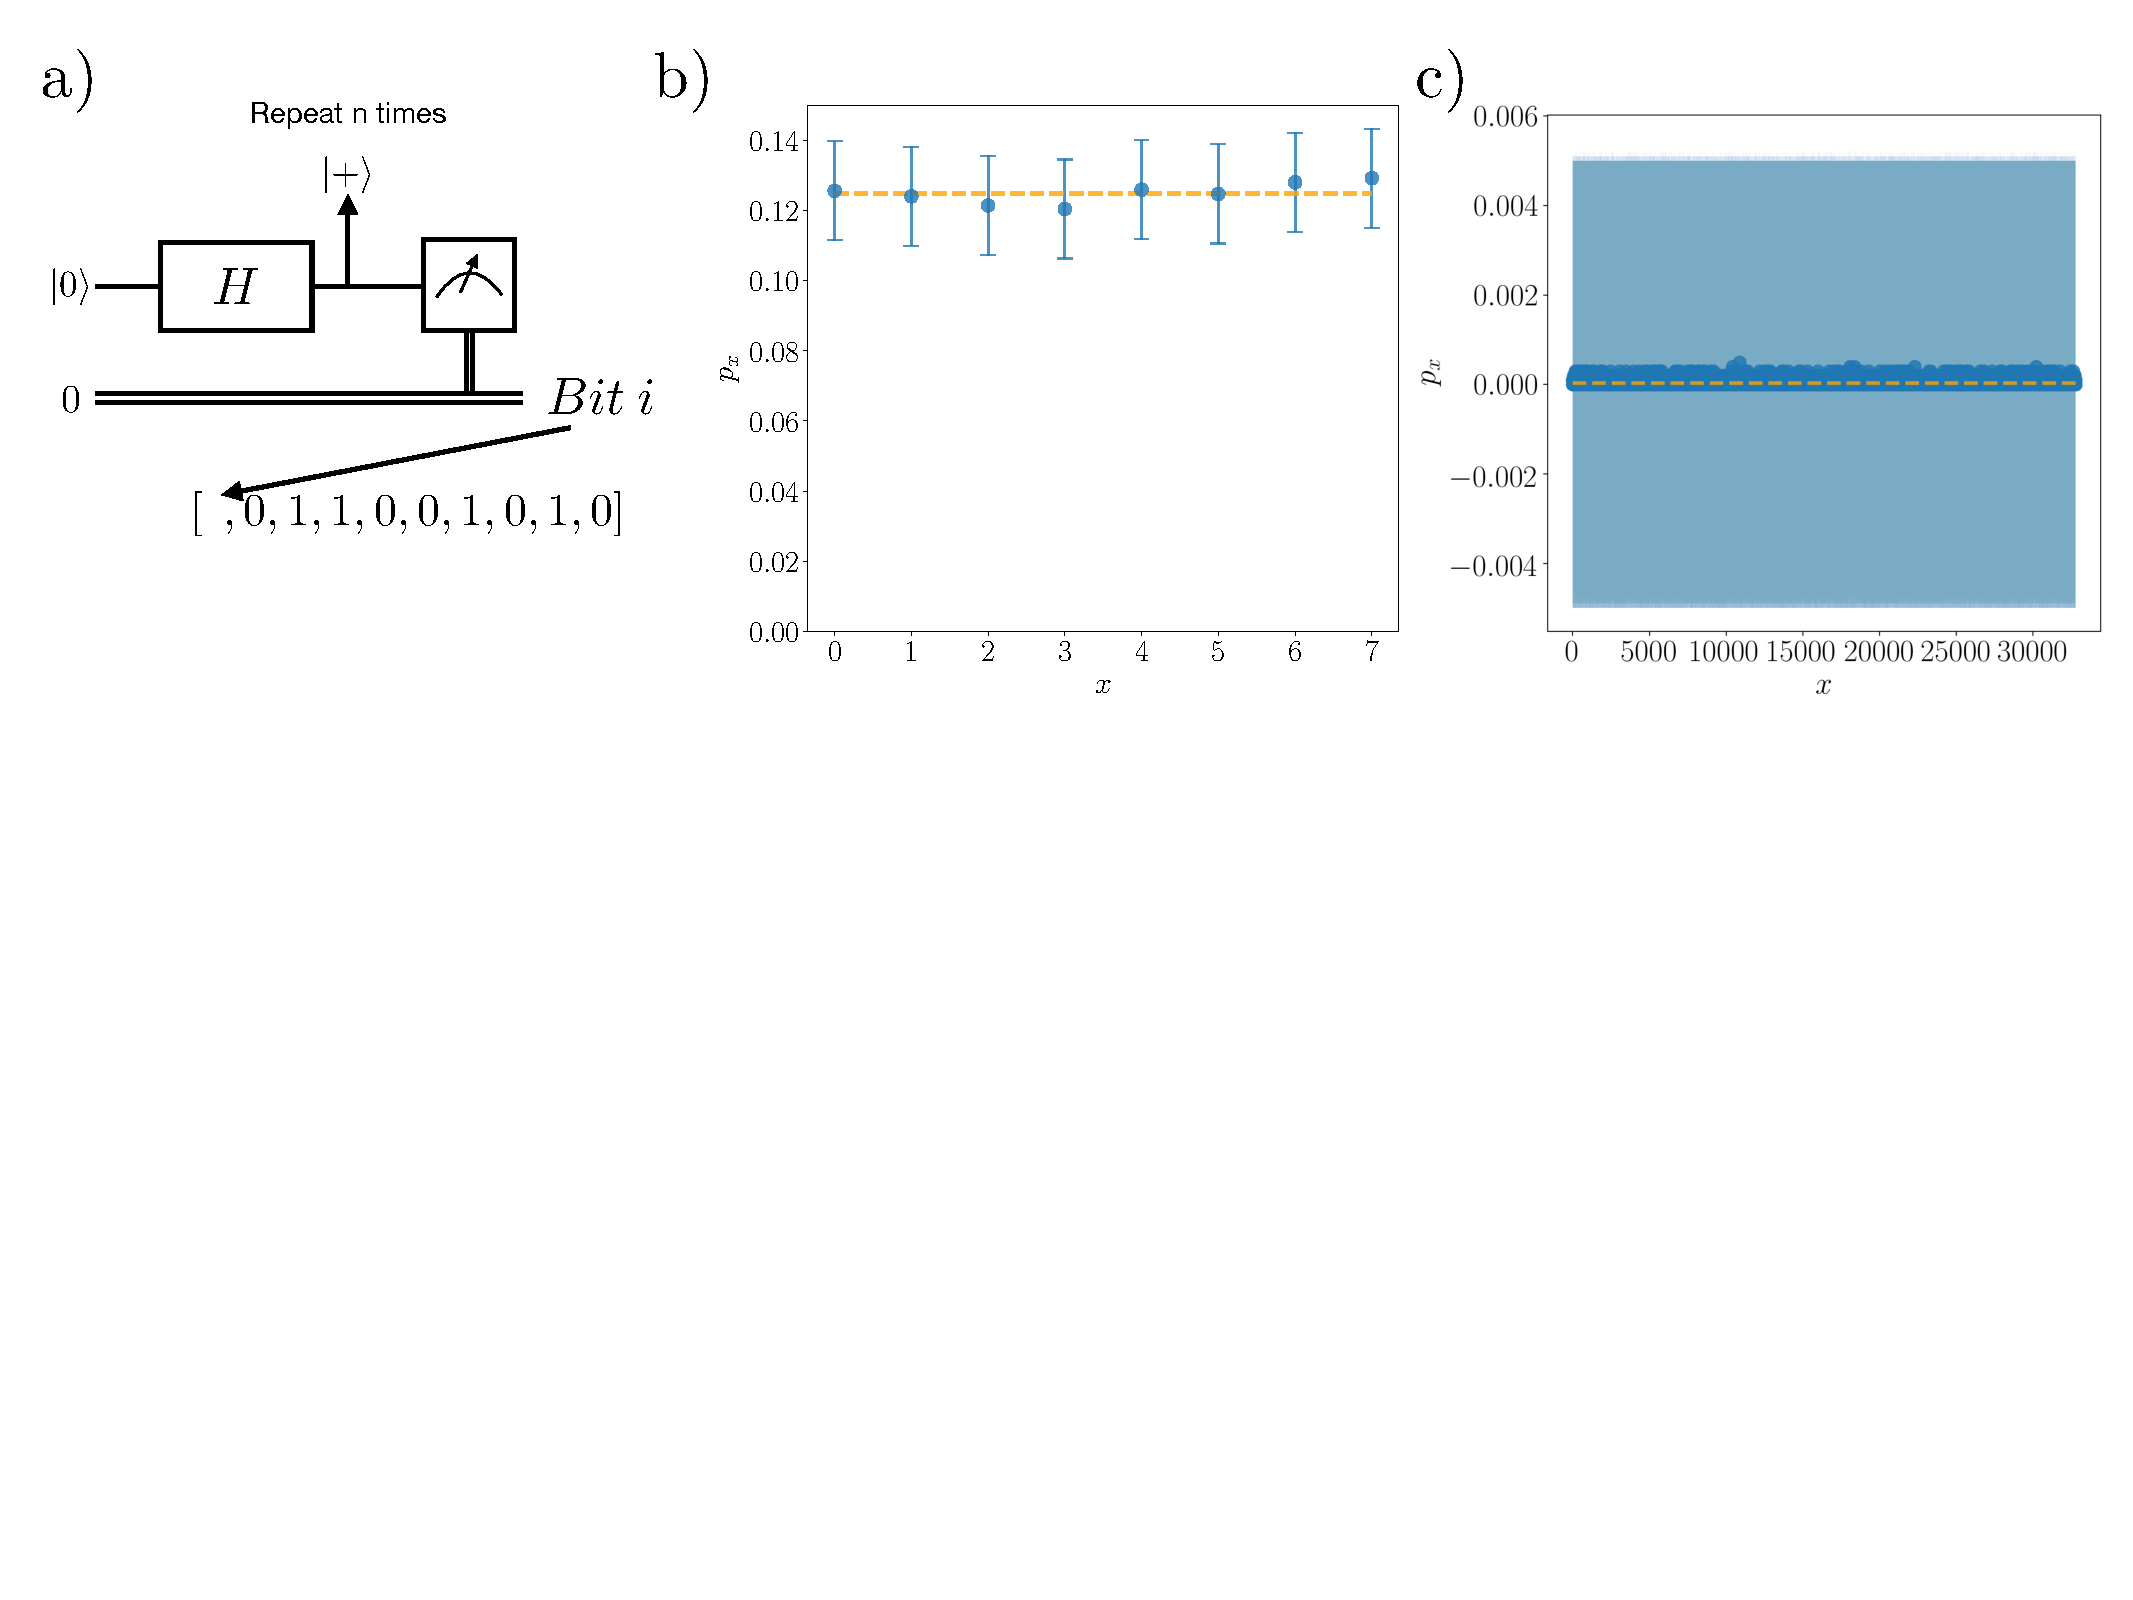
\includegraphics[width=0.95\textwidth]{plot1.pdf}
       \caption{\label{FIG_01: Plot1} \textbf{a)} Schematic representation of the procedure followed to generate random numbers. \textbf{b)} Probability distribution of obtaining number $x$ with our random number generator if $n = 3$. Orange dashed line represents the expected value for the probability of obtaining each number: $1/2^n$. \textbf{c)} Probability distribution of obtaining number $x$ with our random number generator if $n = 15$. The blue cloud are the error bars. Orange dashed line represents the expected value for the probability of obtaining each number: $1/2^n$} 
    \end{figure*} 
    
In order to test our random number generator put it under two standard tests: the fist one is analyzing if the distribution is uniformly sampled and the second one is making sure that samples are not correlated to each other. By samples, bits corresponding to the same random number are not correlated to each other.

Figure \ref{FIG_01: Plot1} b) and c) show the probability of generating random number $x$ between 0 and $2^n$ for $n = 3$ (panel c)) and for $n = 15$ (panel c)). Note this probability distributions should be flat and have a probability of $1/2^n$. The error bars correspond to $1/\sqrt{samps}$ according to the central limit theorem, where $samps = 10^3$ is the number of random numbers generated. Note that for $n = 15$ the error bars are much larger than the actual probability. This is due to the fact that the number of possible outputs of the random number generator is exponentially large and in order to do a good sampling of the probability distribution we would need to collect exponentially many samples, which we cannot do with our laptops. However, both for $n = 3$ and $n = 15$, the simulated values of the probabilities agree with the uniform probability distribution within the error bars.

The second check our random number generator needs to pass is that the samples are not correlated to each other. Pseudo-random number generators satisfy this condition, so this does not prove pure randomness (because it is impossible to test in a classical computer) but it is a sanity check random numbers should satisfy. To test it, within the same random number, we will compute the correlation between two bits and average over the number of samples taken:
\begin{equation}
    C_{i,j} = \langle (x_i-x_j)^2 \rangle-\langle x_i^2 \rangle -\langle x_j^2 \rangle
\end{equation}
where $x_i$ and $x_j$ are the bits in relevant positions $i$ and $j$ of random number $x$. Figure \ref{FIG_02: Plot2} shows the average correlations for $n = 3$ and $n = 15$ averaged over $samps = 10^3$ random numbers. It proves that within the error bars, the correlations are zero and therefore our random number generator does not generate correlated bits. \textbf{All the code to generate the correlation maps and to collect the statistics is attached as a Jupyter Notebook.}

\begin{figure*}[htbp]
        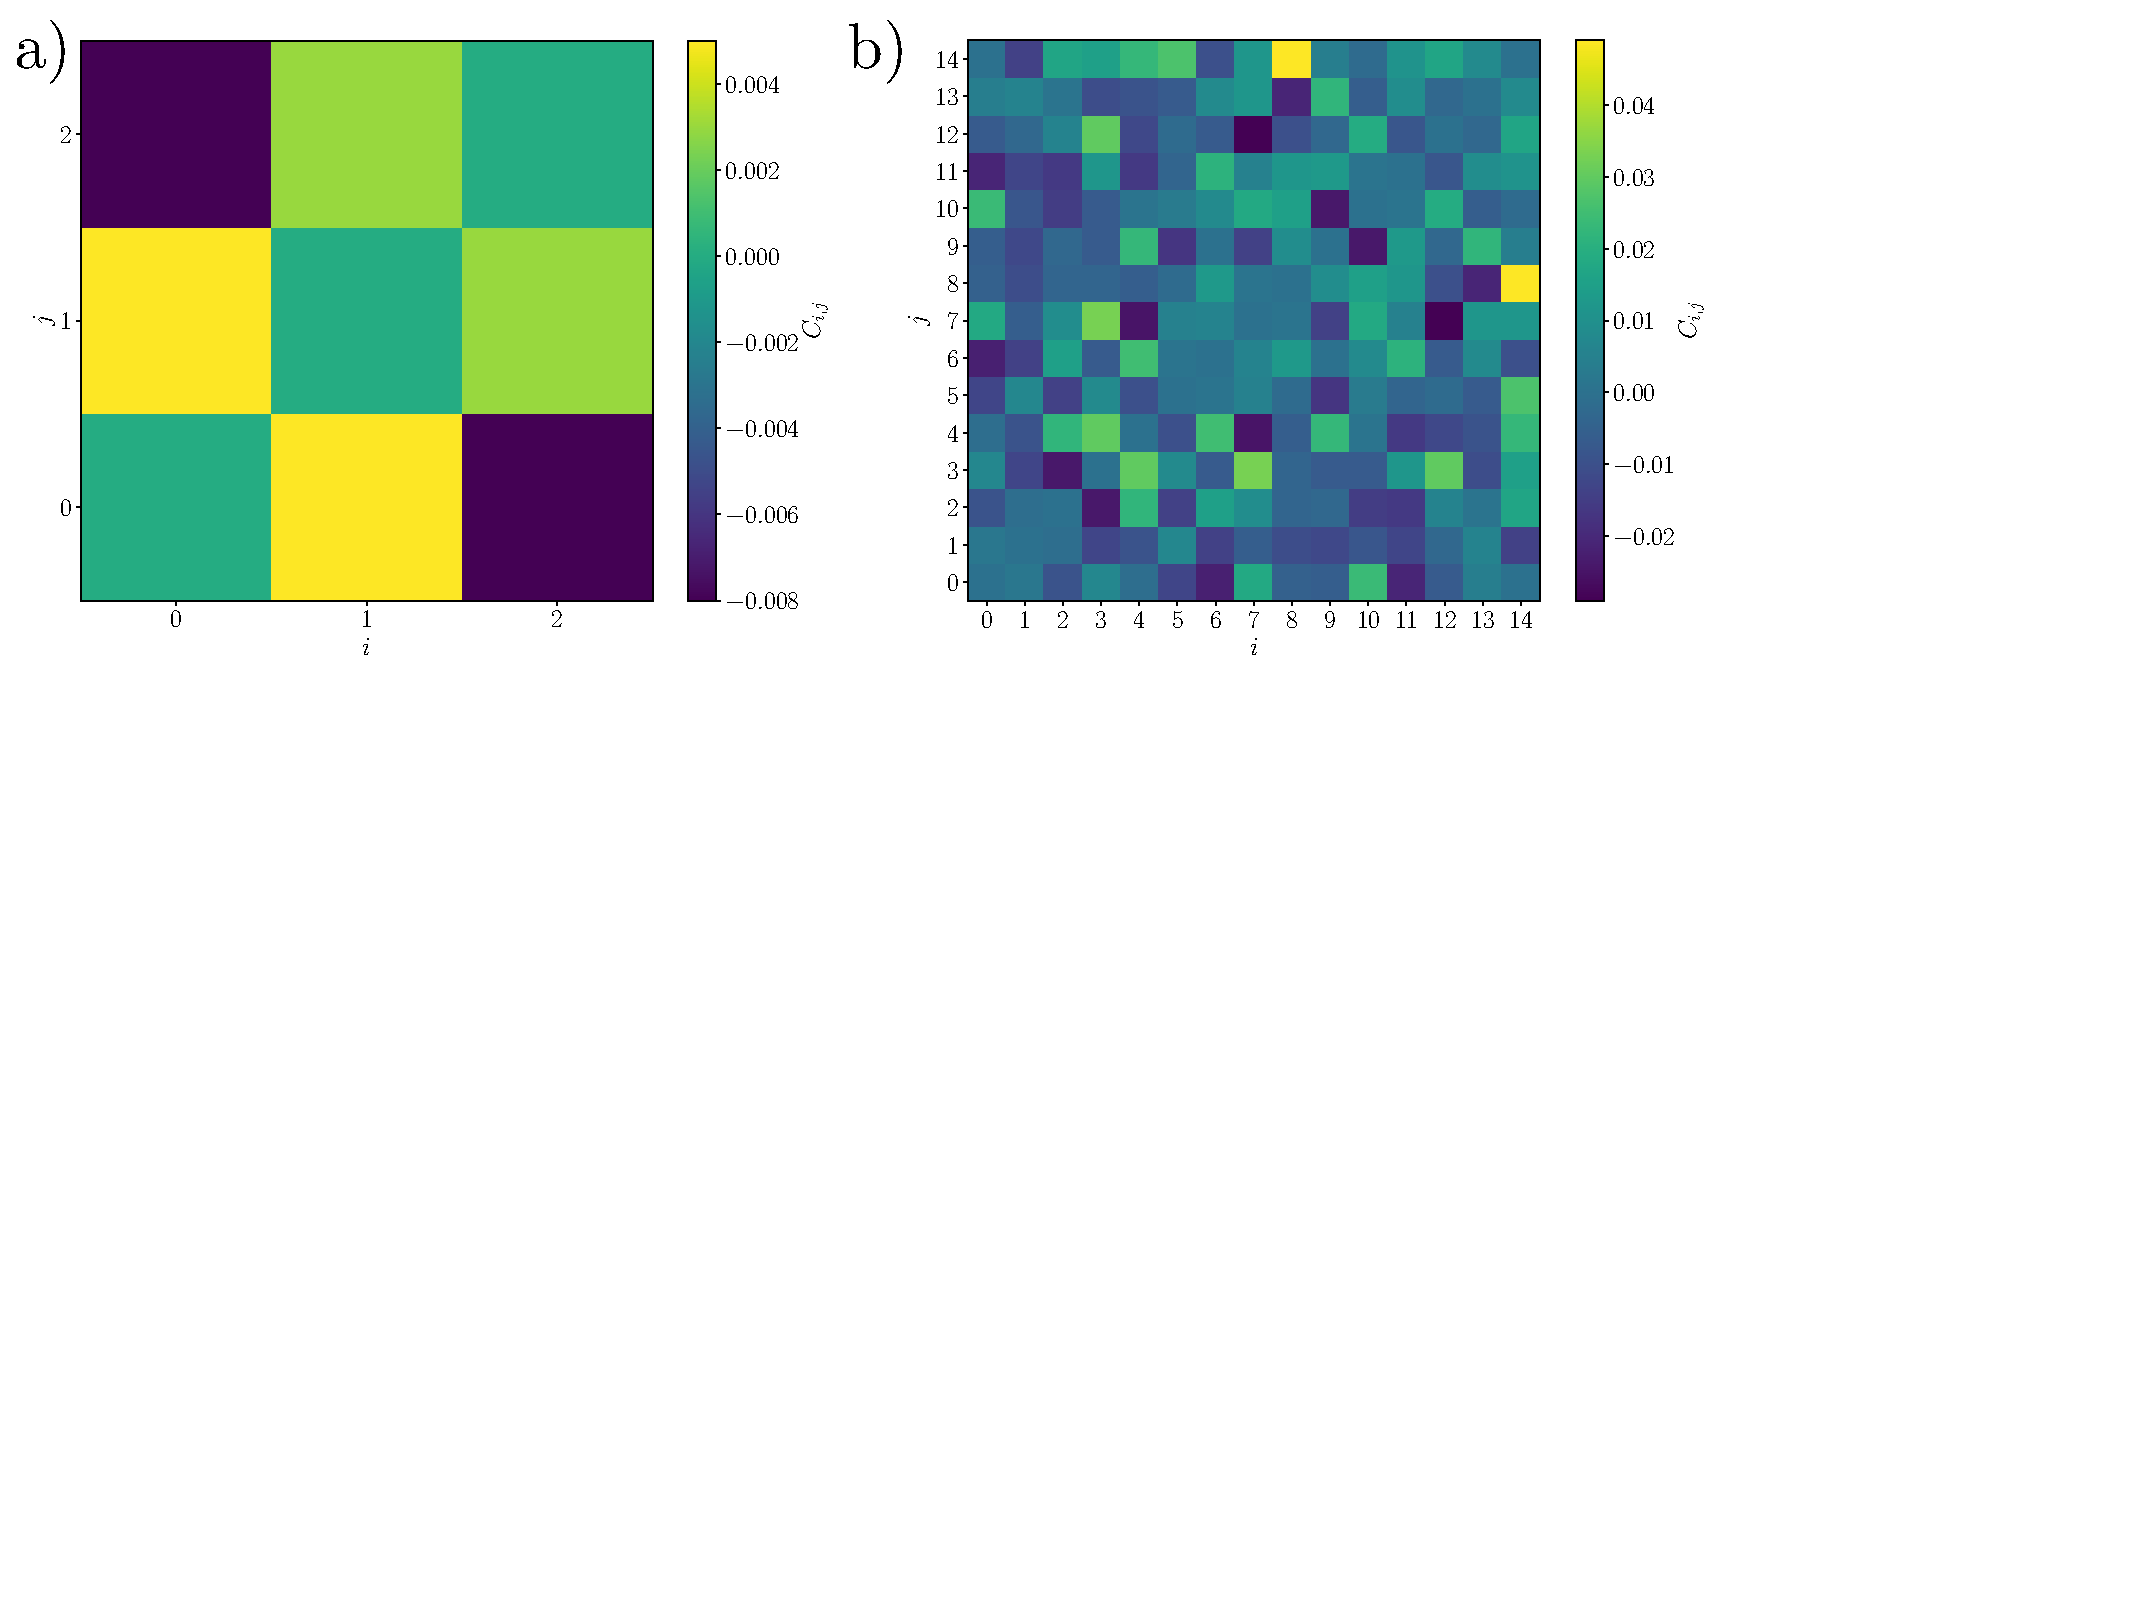
\includegraphics[width=0.95\textwidth]{plot2.pdf}
       \caption{\label{FIG_02: Plot2} \textbf{a)} $n = 3$ \textbf{b)} $n = 15$. Correlation between bits $i$ and $j$ of a given random number, averaged over all the random numbers generated $samps = 10^3$} 
    \end{figure*} 

%%%%%% --------------------- Q14

\subsection*{Q14}


Here we prove the optimal quantum strategy to the CHSH game. We assume the following rules:
\begin{enumerate}
    \item Alice and Bob agree on strategy. Thereafter, they can perform local operations, but they cannot communicate classically.
    \item Alice and Bob respectively receive a random bit $x$ and $y$ from the referee.
    \item Alice and Bob respectively return bits $a$ and $b$ to the referee.
    \item Alice and Bob win iff
        \begin{equation}
            a + b = xy \mod 2.
            \label{eq:chsh-win-condition}
        \end{equation}
\end{enumerate}

We first consider the classical case. In the win condition, $a + b = 1 \Leftrightarrow a \neq b$. Similarly, $xy = 1 \Leftrightarrow x = y = 1$. If all bits are chosen at random, the former condition occurs with probability 1/2, while the latter occurs with probability 1/4. The following truth table then enumerates all possible outcomes and their probabilities:
\begin{equation}
\begin{tabular}{c|c|c||c}
    $a \neq b$ & $x = y = 1$ & Win & Prob. \\
    \hline\hline
    T & T & T & 1/8 \\
    T & F & F & 3/8 \\
    F & T & F & 1/8 \\
    F & F & T & 3/8
\end{tabular}
\label{eq:chsh-truth-table}
\end{equation}
Therefore, if Alice and Bob choose $a$ and $b$ uniformly at random, they win with probability 1/2. The optimal classical strategy is for Alice and Bob to agree beforehand to always choose $a=b$ (either both 0 or both 1, always). This eliminates the first two rows of the table (where they are likely to lose), and they win with probability 3/4. We show that this is optimal by considering Alice's point of view (Bob's is symmetric) in the absence of any strategy. Note that the value of $x$ contains no information as to how she should choose $a$: if $x=1$, the probabilities in each row are unaffected (since she doesn't know $y$), while if $x=0$, only the second and fourth rows remain, where they still win and lose with equal probability. Therefore, Alice needs knowledge of $b$ so she can choose the fourth row in the case $x=0$. If she has \emph{perfect} knowledge of $b$, they will always win in this case (by choosing $a=b)$, while they can still only win 1/2 of the cases where $x=1$. Since $x=0$ (always win) and $x=1$ (win 1/2) are equally likely, they win with probability 3/4, and any uncertainty in $b$ will only reduce their win percentage in the $x=0$ case.

The optimal quantum strategy is obtained as follows. While Alice and Bob are strategizing before the game begins, they share a Bell state
\begin{equation}
\ket{\Psi^+} = \frac{\ket{00} + \ket{11}}{\sqrt{2}}.
\label{eq:chsh-bell-state}
\end{equation}
They also define the orthonormal single-qubit measurement basis
\begin{equation}
\begin{aligned}
    \ket{\mu_0(\theta)} &= \cos\theta\ket{0} + \sin\theta\ket{1} \\
    \ket{\mu_1(\theta)} &= \sin\theta\ket{0} - \cos\theta\ket{1}
\end{aligned}
\label{eq:chsh-measurement-basis}
\end{equation}
and agree to choose their angles based on the respective values of the referee bits $x$ and $y$:
\begin{equation}
\begin{aligned}
\text{Alice:} &\quad \begin{cases}
    x = 0 \implies \theta = \alpha_0\\
    x = 1 \implies \theta = \alpha_1
\end{cases}\\
\text{Bob:} &\quad \begin{cases}
    y = 0 \implies \theta = \beta_0\\
    y = 1 \implies \theta = \beta_1.
\end{cases}
\end{aligned}
\label{eq:chsh-angle}
\end{equation}
Finally, they agree to choose their respective answer bits $a$ and $b$ by measuring the Bell state \eqref{eq:chsh-bell-state} in the measurement basis \eqref{eq:chsh-measurement-basis}:
\begin{equation}
\begin{aligned}
\text{Alice:} &\quad \begin{cases}
    \mu_0 \implies a = 0 \\
    \mu_1 \implies a = 1
\end{cases}\\
\text{Bob:} &\quad \begin{cases}
    \mu_0 \implies b = 0 \\
    \mu_1 \implies b = 1.
\end{cases}
\end{aligned}
\label{eq:chsh-answer}
\end{equation}

We now analyze the above strategy. First consider the particular case $(x, y) = (0, 0)$. According to the angle selection rule \eqref{eq:chsh-angle}, Alice uses the measurement basis $\{\ket{\mu_0(\alpha_0)}, \ket{\mu_1(\alpha_0)}\}$ while Bob uses $\{\ket{\mu_0(\beta_0)}, \ket{\mu_1(\beta_0)}\}$. According to the win condition \eqref{eq:chsh-win-condition}, they win if $(a, b) \in \{(0, 0), (1,1)\}$. According to the answer-bit selection rule \eqref{eq:chsh-answer}, these correspond to measurement outcomes $(\mu_a, \mu_b) \in \{(\mu_0, \mu_0), (\mu_1, \mu_1)\}$, which occur with probability,
\[\Pr(\text{win}|x,y=0,0) =
\abs{\braket{\mu_0(\alpha_0)\mu_0(\beta_0)}{\Psi^+}}^2 +
\abs{\braket{\mu_1(\alpha_0)\mu_1(\beta_0)}{\Psi^+}}^2\]

In more generality, for the cases $(x, y) \in \{(0, 0), (0, 1), (1, 0)\}$ corresponding to rows of the truth table \eqref{eq:chsh-truth-table} where $x = y = 1$ is False (denote this condition $C$), they win if $a = b$, which occurs with probability
\[\Pr(\text{win}|C=\text{False}) = \sum_{a=b}
\abs{\braket{\mu_a(\alpha_x)\mu_b(\beta_y)}{\Psi^+}}^2.\]
In the remaining case, $(x, y) = (1, 1)$ (i.e. $C$ is True), they win if $a \neq b$, which occurs with probability
\[\Pr(\text{win}|C=\text{True}) = \sum_{a\neq b}
\abs{\braket{\mu_a(\alpha_1)\mu_b(\beta_1)}{\Psi^+}}^2.\]
Using \eqref{eq:chsh-bell-state} and \eqref{eq:chsh-measurement-basis} we compute these probabilities explicitly as
\begin{align}
\Pr(\text{win}|x,y=0,0) &= \cos[2](\alpha_0 - \beta_0) \\
\Pr(\text{win}|x,y=0,1) &= \cos[2](\alpha_0 - \beta_1) \\
\Pr(\text{win}|x,y=1,0) &= \cos[2](\alpha_1 - \beta_0) \\
\Pr(\text{win}|x,y=1,1) &= \sin[2](\alpha_1 - \beta_1)
\end{align}
Since $x$ and $y$ are chosen uniformly at random, the total win probability is
\begin{equation}
    \Pr(\text{win}) = \frac{1}{4}\left(
    \cos[2](\alpha_0 - \beta_0) +
    \cos[2](\alpha_0 - \beta_1) +
    \cos[2](\alpha_1 - \beta_0) +
    \sin[2](\alpha_1 - \beta_1)\right).
\end{equation}
Extremizing with respect to each angle yields the conditions,
\begin{align}
    \pdv{\Pr}{\alpha_0} = 0 &\implies \sin 2(\alpha_0 - \beta_0) + \sin 2(\alpha_0 - \beta_1) = 0 \\
    \pdv{\Pr}{\alpha_1} = 0 &\implies \sin 2(\alpha_1 - \beta_0) - \sin 2(\alpha_1 - \beta_1) = 0 \\
    \pdv{\Pr}{\beta_0} = 0 &\implies \sin 2(\alpha_0 - \beta_0) + \sin 2(\alpha_1 - \beta_0) = 0 \\
    \pdv{\Pr}{\beta_1} = 0 &\implies \sin 2(\alpha_0 - \beta_1) - \sin 2(\alpha_1 - \beta_1) = 0,
\end{align}
which are satisfied for $\alpha_0 = 0$, $\alpha_1 = \pi/4$, $\beta_0 = \pi/8$, and $\beta_1 = -\pi/8$. These choices for the angles then yield the optimal strategy, and the win probability reduces to
\[\Pr(\text{win}) = \cos[2](\frac{\pi}{8}) \approx 85\%.\]

\end{appendices}

\clearpage\newpage
\nocite{*}
\bibliographystyle{plainnat}
\bibliography{references}
\end{document}